\documentclass{sigchi}

% Load basic packages
\usepackage{balance}       % to better equalize the last page
\usepackage{graphics}      % for EPS, load graphicx instead 
\usepackage[T1]{fontenc}   % for umlauts and other diaeresis
\usepackage{txfonts}
\usepackage{mathptmx}
\usepackage[pdflang={en-US},pdftex]{hyperref}
\usepackage{color}
\usepackage{booktabs}
\usepackage{textcomp}
\usepackage{url}
\usepackage{pdfpages}
%\usepackage[section]{placeins}
\usepackage{float}


% Some optional stuff you might like/need.
\usepackage{microtype}        % Improved Tracking and Kerning
% \usepackage[all]{hypcap}    % Fixes bug in hyperref caption linking
\usepackage{ccicons}          % Cite your images correctly!

\usepackage{todonotes}

\def\plaintitle{CS 649 Final Report - Team Billie}
\def\plainauthor{First Author, Second Author, Third Author,
  Fourth Author, Fifth Author, Sixth Author}
\def\emptyauthor{}
\def\plainkeywords{Authors' choice; of terms; separated; by
  semicolons; include commas, within terms only; required.}
\def\plaingeneralterms{Documentation, Standardization}

% llt: Define a global style for URLs, rather that the default one
\makeatletter
\def\url@leostyle{%
  \@ifundefined{selectfont}{
    \def\UrlFont{\sf}
  }{
    \def\UrlFont{\small\bf\ttfamily}
  }}
\makeatother
\urlstyle{leo}

% To make various LaTeX processors do the right thing with page size.
\def\pprw{8.5in}
\def\pprh{11in}
\special{papersize=\pprw,\pprh}
\setlength{\paperwidth}{\pprw}
\setlength{\paperheight}{\pprh}
\setlength{\pdfpagewidth}{\pprw}
\setlength{\pdfpageheight}{\pprh}

% Make sure hyperref comes last of your loaded packages, to give it a
% fighting chance of not being over-written, since its job is to
% redefine many LaTeX commands.
\definecolor{linkColor}{RGB}{6,125,233}
\hypersetup{%
  pdftitle={\plaintitle},
  pdfauthor={\emptyauthor},
  pdfkeywords={\plainkeywords},
  pdfdisplaydoctitle=true, % For Accessibility
  bookmarksnumbered,
  pdfstartview={FitH},
  colorlinks,
  citecolor=black,
  filecolor=black,
  linkcolor=black,
  urlcolor=linkColor,
  breaklinks=true,
  hypertexnames=false
}

% create a shortcut to typeset table heaOIings
% \newcommand\tabhead[1]{\small\textbf{#1}}

% End of preamble. Here it comes the document.
\begin{document}
\title{\plaintitle}

\numberofauthors{3}
\author{%
  \alignauthor{Yilun Bai \\
    \affaddr{Computer Science}\\
    \email{yilun.bai@uwaterloo.ca}}\\
\alignauthor{Yananan Wang \\
    \affaddr{Computer Science}\\
    \email{y3248wan@uwaterloo.ca}}\\
% \alignauthor{3rd Student Name \\
%    \affaddr{Department}\\
%   \email{uwaterloo e-mail address}}\\
}

\maketitle

\section{1. Description of the project}

With economic progress and social development, personal finance management has become more and more important in our daily life. As a responsible adult living in modern society, properly managing personal finance is a fundamental to form social trust and a stable economy. Allied Market Research has published a report \cite{AMR} and said, "Increasing need to track and manage income, growing dependency on the Internet, spiraling use of mobile applications, and rising adoption of personal finance software across developing economies are expected to propel the growth of the global personal finance software market". Therefore, the general market segment we are targeting is personal finance software market.

Have any of the followings ever happened to either you or someone you know? You subscribed to Apple Music when using an iPhone and a MacBook, but later switched to use an Android phone and a Windows laptop with Spotify subscription, but forgot to cancel the Apple Music subscription after 6 months of extra auto-charges; You want to change the payment option of your auto-pay for your mobile phone bill, but you forget the payment website or your username and password; You pay the full amount of the utility bill and forget that it is supposed to be split by 50/50 with your roommate; Or you just simply too busy at the end of a month and totally forget to pay your rent, only realize later by a email from the landlord with a late payment penalty fee that you are definitely not willing to pay. Paying bills has become a tedious routine happening every certain period of time, either weekly, monthly, or yearly. In addition,the bills we need to pay have also been expanded into various categories, and not all the bills are due on the same day, nor do they have the same amount, even where and how we should pay varies from bill to bill. Gradually, we lose track of what we're paying for and sometimes waste our money on it or even cause a more significant impact on our daily life. Therefore, the problem we want to address is decentralized management of bills. 

As a result, we are motivated to build a bill management mobile application for our project to address those problems and to improve the user experience on the whole bill management and payment process. Our project is named "Billie", as in a personal bill management assistant for users. It could also be interpreted to be the abbreviation of "Bill Is Easy". It addresses the above problem by centralizing different problems faced in bill management into one single application and providing separate solutions to resolve them. With compactness, simplicity, and multi-functionality of Billie, the important potential contribution is that it would help people to develop a bill management habit by using this simple tool and bringing up the societies life satisfaction by allowing people better keep track of their living expenses. 

\section{2. Goals of the project}

We want to focus on the bill management of the market segment and the specific goals of the project will be discussed in the following part. 

To begin with, we want to allow users to better keep track of their bills, and let people be aware of the automatic payments that will occur beforehand so that the user can choose if they want to continue being a subscriber. Besides, we want to simplify the payment process and centralize different bill payment approaches, and therefore save users' time and effort. In addition, we want to avoid late payment situations as far as possible, so that people will not forget to pay bills and don't have to pay penalty fees as well. Besides, regarding bill splitting, we want to avoid conflicts between primary payers and other co-payers in bill sharing process, and try to include them into the same information flow. 

\section{3. Product anticipated users}

Based on the data and Figure~\ref{fig:figure1} from Statistics Canada, the Consumer Spending in Canada averaged around 584002 CAD million from 1961 to 2018 with an increasing trend, and it reaches 1166783 CAD million in 2019 ~\cite{DCCS}. Hence, there are more and more bill payments involved in people's daily life and we want to separate them into different user groups according to the demographics.

\begin{figure}[h!]
\centering
  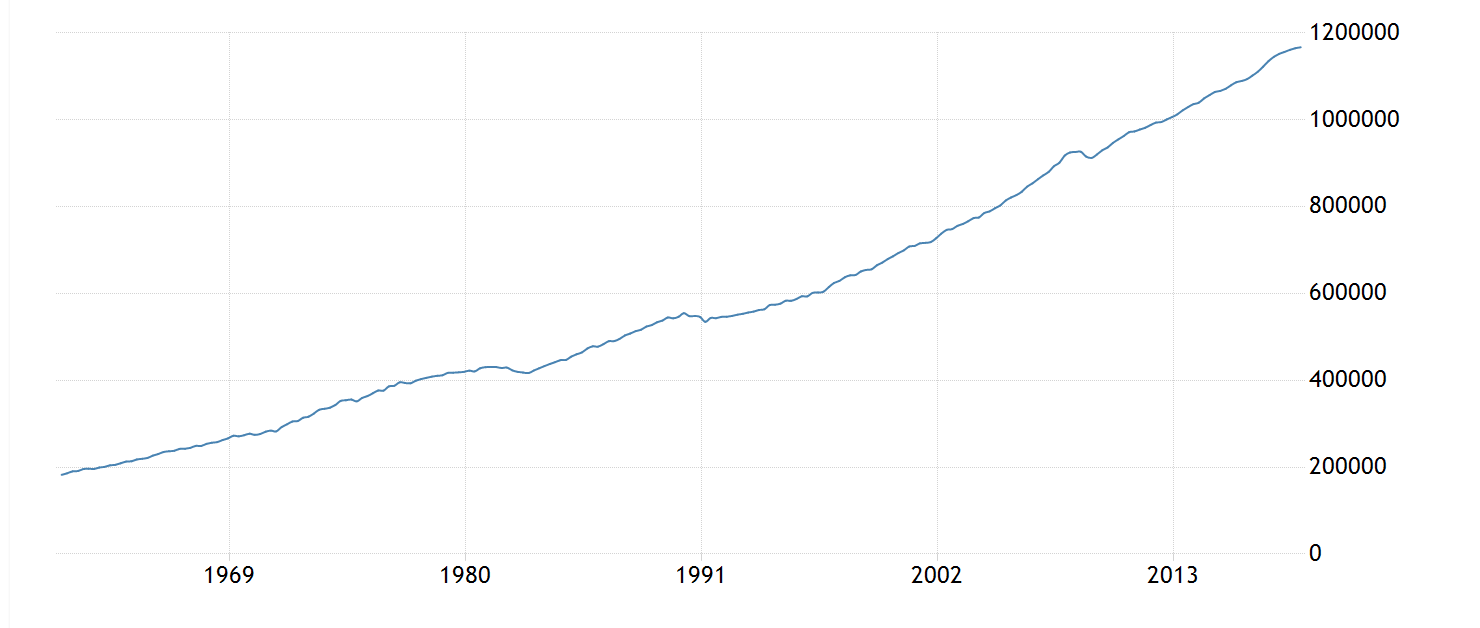
\includegraphics[width=0.9\columnwidth]{consumer-spending.png}
  \caption{Consumer Spending from 1961 to 2018 in Canada}
  \label{fig:figure1}
\end{figure}


\begin{figure*}[h]
\centering
  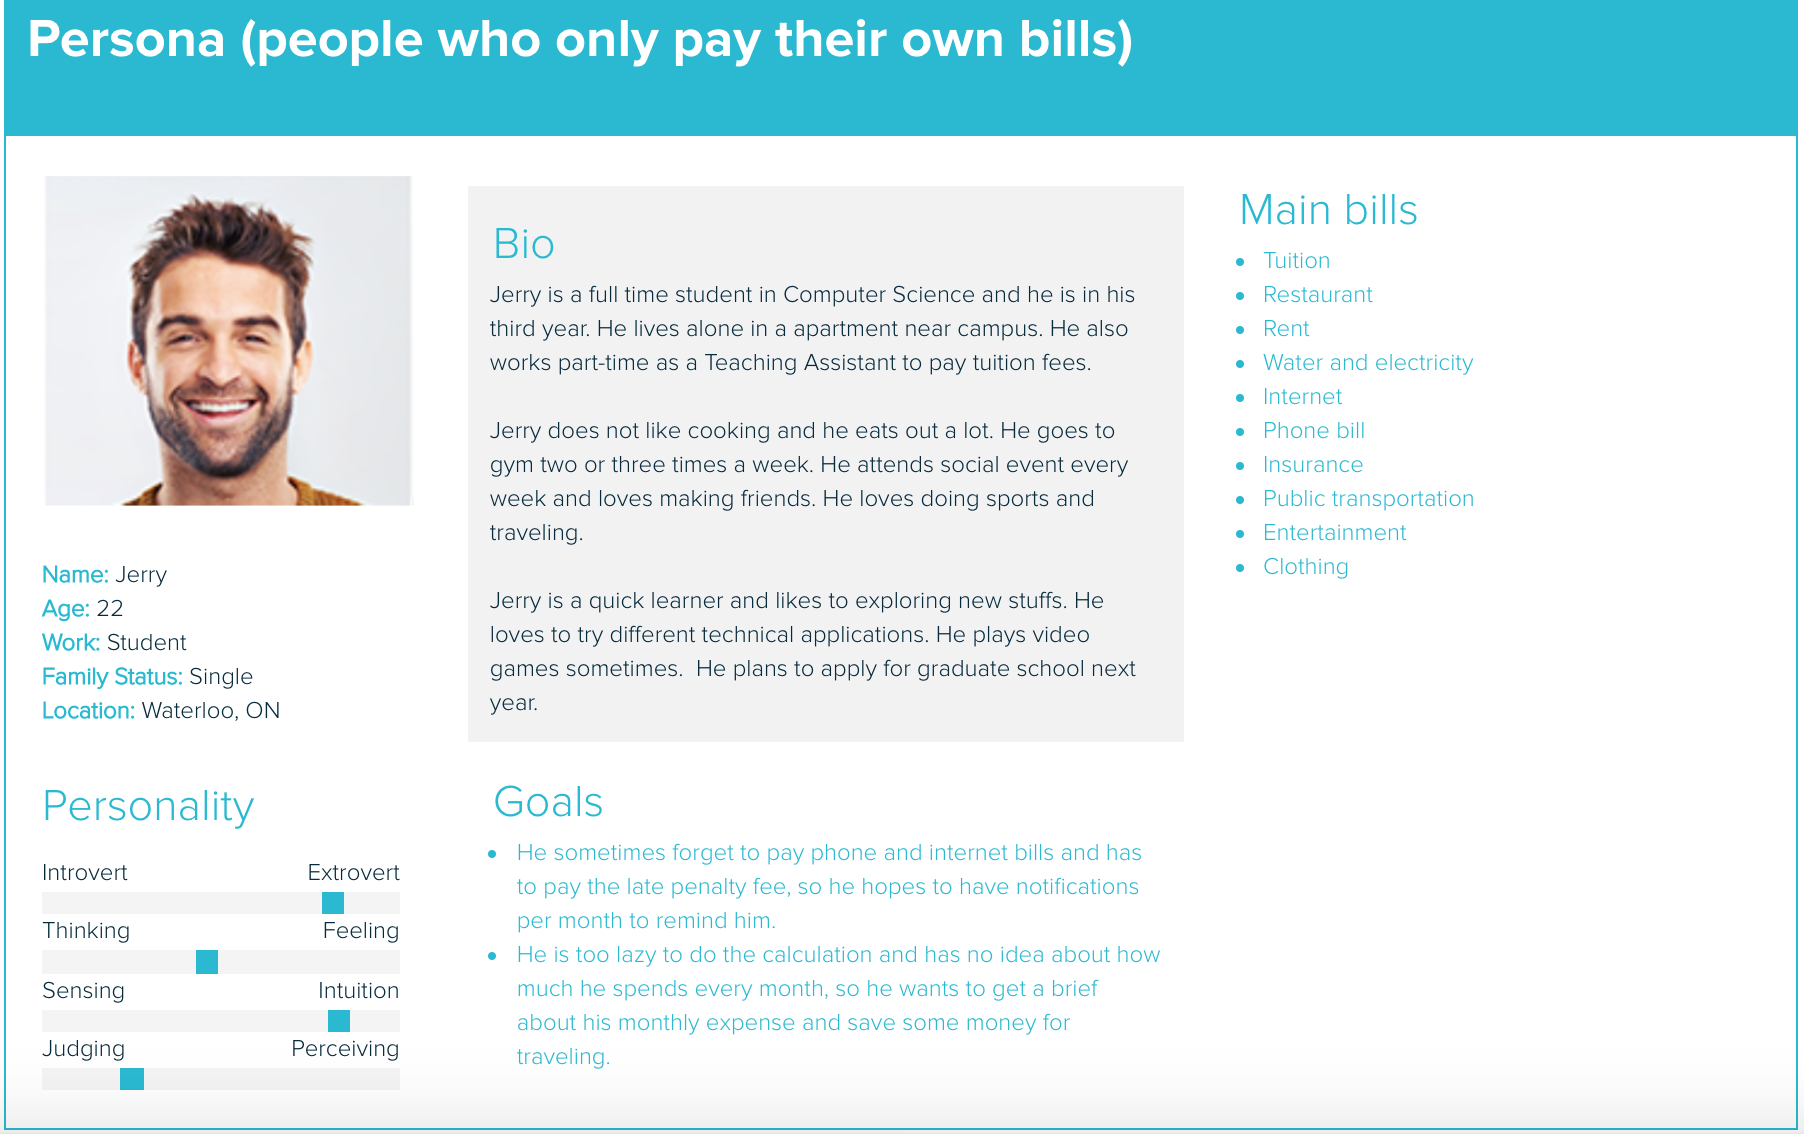
\includegraphics[width=0.7\textwidth,height=7cm]{persona1.png}
  \caption{Persona for the first user group}
  \label{fig:figure2}
\end{figure*}
\begin{figure*}[h]
\centering
  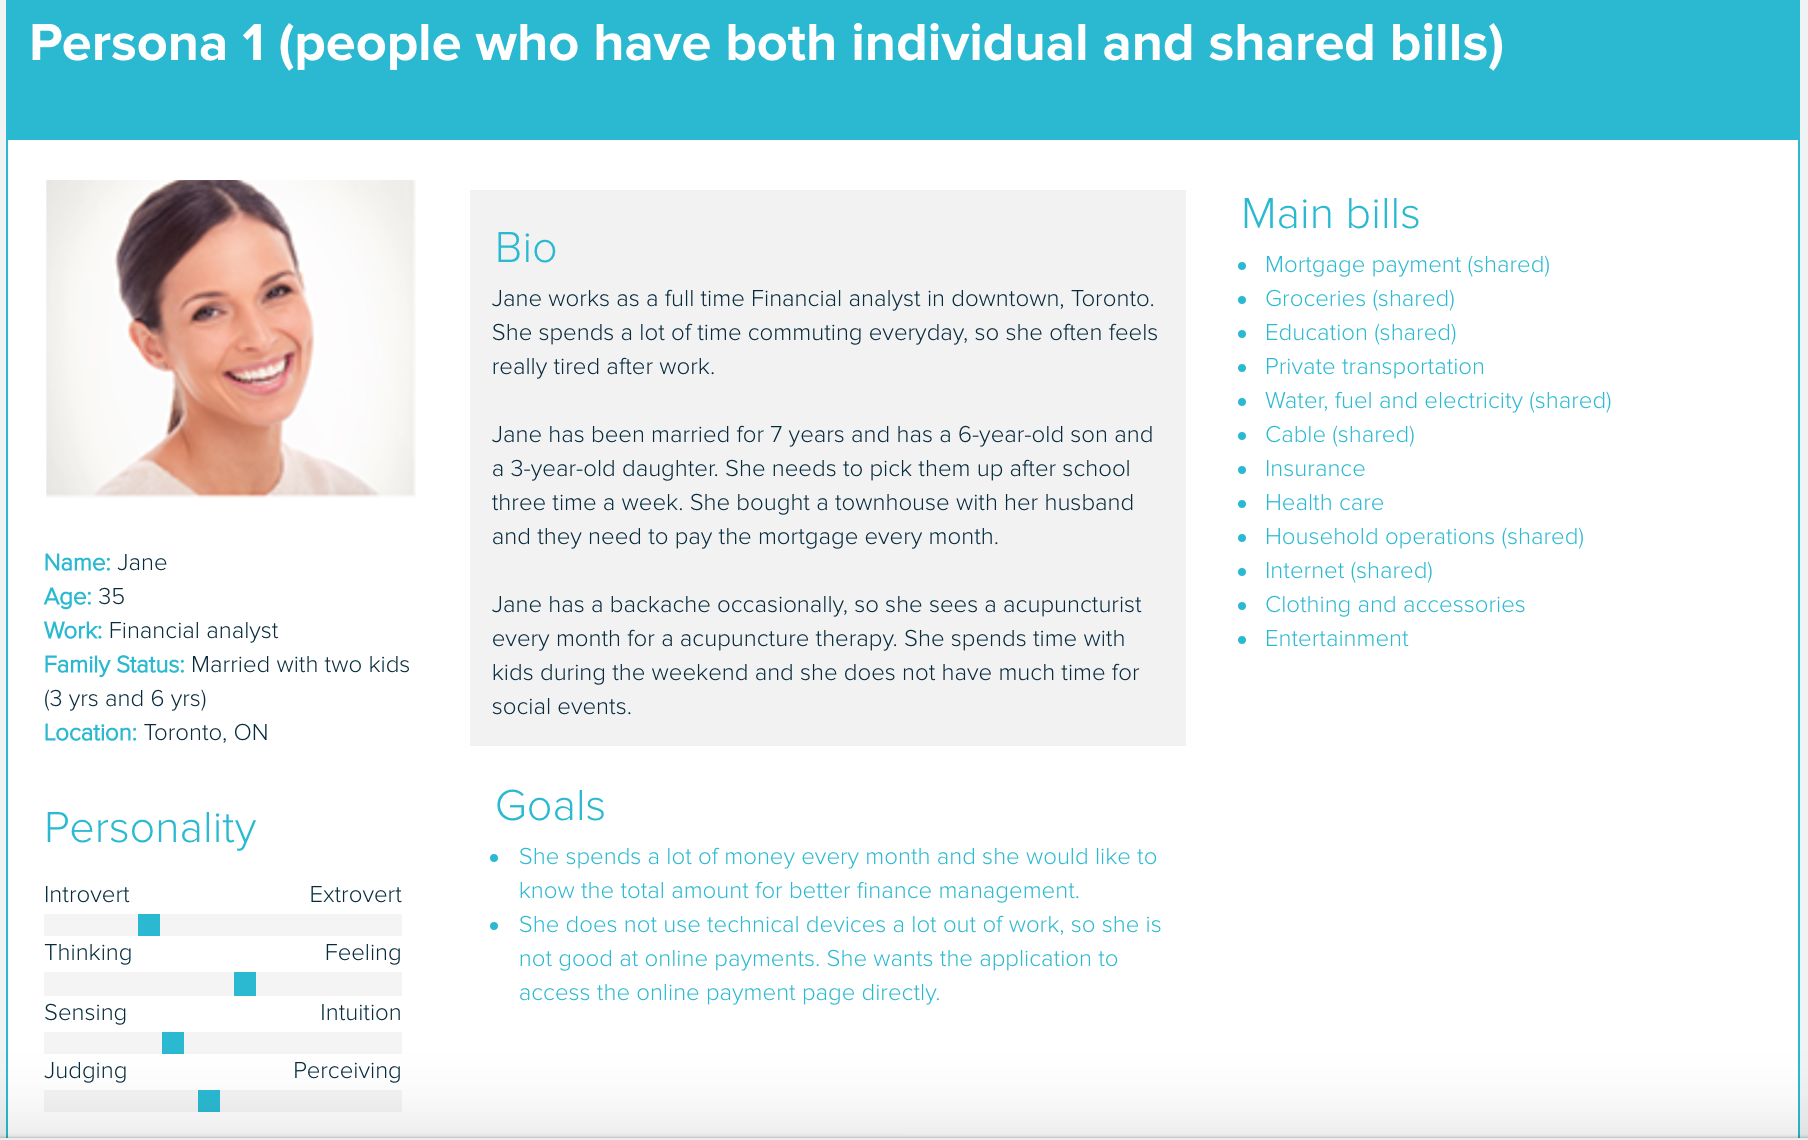
\includegraphics[width=0.7\textwidth,height=7cm]{persona1-1.png}
  \caption{Persona 1 for the second user group}
  \label{fig:figure3}
\end{figure*}
\begin{figure*}[h!]
\centering
  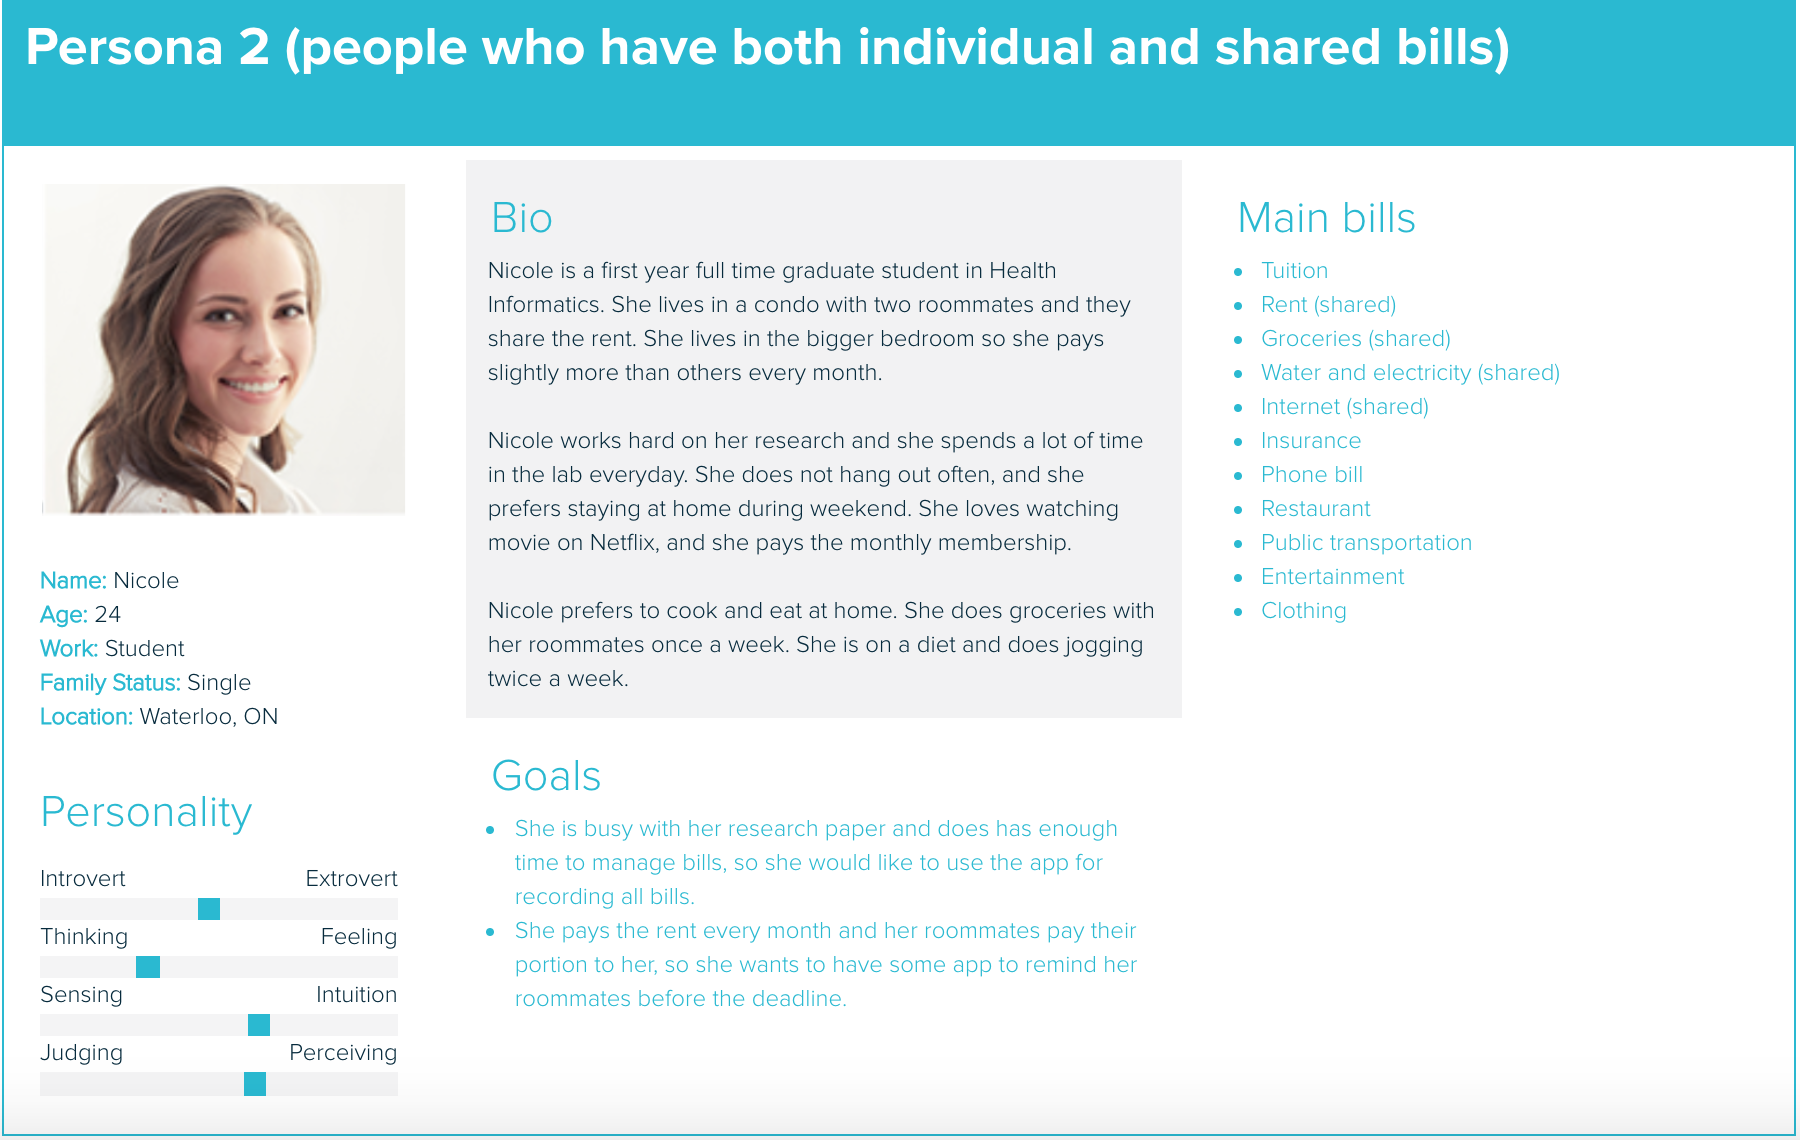
\includegraphics[width=0.7\textwidth,height=7cm]{persona1-2.png}
  \caption{Persona 2 for the second user group}
  \label{fig:figure4}
\end{figure*}

 In terms of age, it does not matter so much since every adult would have some bills to manage and age has no impact on that. Also, for the same reason, gender does not make a difference, either. Besides, people with different income amounts may have different types of bills, but it does not affect functionalities of the application. In addition, residence does not make a great difference, since where do people live has little impact on their bills. Furthermore, other characteristics such as means of transportation and food preference are not considered as key influential points in this application, either. 
 

 Therefore, based on who pays the bills, all the users can be separated into two user groups, which are "people who only pay their own personal bills" and "people who have both individual and shared bills". People who have shared bills will have the extra functionality to jointly manage their bills with other people.
 
 
According to the data from Statistics Canada about Kitchener-Cambridge-Waterloo area ~\cite{ECP} and other statistical information ~\cite{FHSC}, we would like to create personas to represent the two user groups described above. The first user group will be illustrated with one persona as shown in Figure~\ref{fig:figure2}, while the second user group will have two personas (Persona 1 in Figure~\ref{fig:figure3} and Persona 2 in Figure~\ref{fig:figure4}) since we want to focus more on people with shared bills. Each persona includes the basic demographics, a bio description about social environment and personalities, as well as the goals when he/she is using the product.

According to the personas created, we would like to select the second user group as target users, because there are a variety of shared bills and the functionality of managing those bills is desired by a larger group of users. In addition, we want to aim at the persona 2 of this user group since it is easier to recruit participants from this category. Therefore, we will select 3-5 participants within 18 to 40 years old from Waterloo-Kitchener Area, Canada. In addition, it is required that all the participants have shared bills with others because it is the key characteristic of our target user group. To make the study generalizable, all the participants should be students with at least one roommate. Also, it is better to choose participants with different education levels (i.e. Undergraduate, Graduate, and Doctor) to get some diverse results. Besides, gender does not make a great difference in this case, so we will select both male and female participants. Furthermore, other demographics such as income, family status do not matter so much in this study, so we can try to find participants with various income or family statuses.


\section{4. Exploratory study}
\subsection{4.1 Description of goals, hypotheses and focus}

Through the exploratory user study, we wish to get a general view of users' previous experience using bill management application as well as their prior beliefs about bill management. Other than that, we would like to have an overview of the main types of bills people are dealing with either periodically or for one time. Besides, since our target user group is people with shared bills, we want to hear about details on sharing bills with others. Also, we would like to know the goals they want to achieve by using the app and any features they desire to have. In addition, it is necessary to know their concerns or fears about using bill management apps. 

Other than that, we want verify several hypotheses based on their responses.

\textbf{\textit{Hypothesis 1. People often forget about their bill payments.}}

First of all, people tend to forget. The things they forget about their bills can vary from the due date, the amount, the payment website, the username and password, the payment method, or the bill itself. A survey done by the Pew Research Center in 2007 shows how a regular household expense look like back then as we can see in Figure~\ref{fig:figure5} ~\cite{AWAPF}. As for now, there are so many types of bills to pay in our lives and it becomes hard to keep track of. According to a report by the Aite Group that is sponsored by ACI Worldwide and Visa in 2018, named "U.S. Consumer Payments Experience: A Blueprint for Creating Positive Behaviors," which surveyed 2,425 U.S. consumers, a surprising 46\% of consumers paid a bill late because they either forgot to pay the bill, were short of money, or for another reason in the last 12 months ~\cite{BAABs}.

\begin{figure}[h!]
\centering
  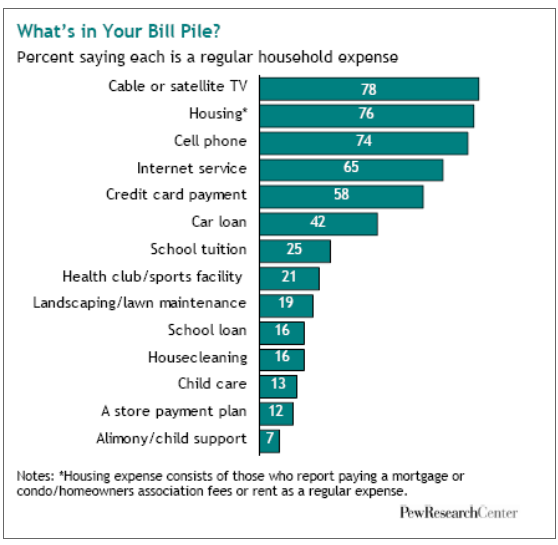
\includegraphics[width=0.9\columnwidth]{types-of-bills.png}
  \caption{Types of bill to pay for a regular American household in 2007}
  \label{fig:figure5}
\end{figure}

\textbf{\textit{Hypothesis 2. Auto-payments and Subscriptions are usually neglected after the initial setup.}}

Secondly, with all the online subscriptions and auto-payments emerging in our lives, it admittedly saves us some trouble to go through the payment process regularly, but other problems are brought up. According to the Forgotten Subscriptions Index from \textit{TopCashback.co.uk} polled from 2,213 UK adults, 29\% of people say they have forgotten they were paying for a subscription service. Figure \ref{fig:figure6} shows that the top 7 unused subscriptions. One in four people has continued to pay for a subscription without realizing the cost had increased, while 46\% forget to cancel after a free trial period. Some 4\% have even unknowingly continued to pay for a subscription for an ex-partner ~\cite{CAYPS}. The problems with those subscriptions are that once people set them up, all the following payments are no longer well noticed by the users since the provider secretly wants you to keep paying.

\begin{figure}[h!]
\centering
  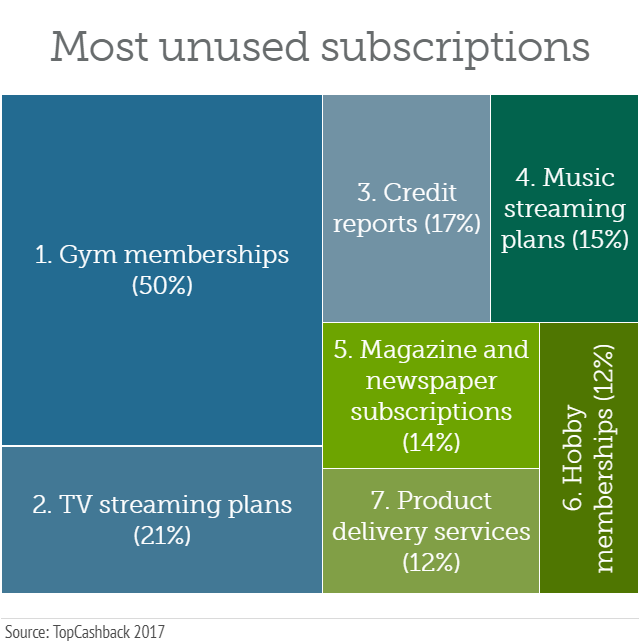
\includegraphics[width=0.9\columnwidth]{unused-sub.png}
  \caption{Top 7 unused subscription }
  \label{fig:figure6}
\end{figure}

\textbf{\textit{Hypothesis 3. People are having trouble splitting their bills with others.}}

Another common issue in bill management is bill sharing. It is often seen with college students who live with roommates, as well as any other who lives together. Bills like rent, electricity, water, internet, groceries, as well as other utilities are often shared between multiple payers. Although there are applications to split bills after the primary payer paid the bill, they are still lack of functionality to make it user-friendly not only to the primary payer, but also to the co-payers. Shared bills are often done by one individual pays the whole amount and the others pay directly to this individual through cash, e-transfer or any other means they are used to which are often not tracked. For things like internet bills that are shared evenly in a household, only the primary account user would receive a notice that an automatic charge is happening and others who pay for a part of this bill has zero acknowledge to it until notified by the primary payer. We want to understand how frequently people split their bills, how the bills are split, and through what means do the other payers pay back the primary payer. 


Therefore, we will mainly get qualitative, attitudinal data and maybe some behavioural data through this study. After we get the results, we will perform analysis and extract useful information from participants' responses. The information can help us understand user's needs, wants, and fears, so we are able to design the app based on the targeting aspects. Also, the actual experience from participants can help us adjust and refine personas so that they are more colorful, detailed and close to real life. Finally, we can know better about users' expectation and build our project accordingly.



\subsection{4.2 Description of participants}

According to our user group, we have selected 4 participants with average age 24-year-old from Waterloo- Kitchener Area, Canada. In addition, all the participants have shared bills with others and at least one roommate by the characteristic of our target user group. Also, in order to get some diverse results, our participants are of different genders (3 male, 1 female), education levels (2 undergraduate, 2 graduate), family status (3 single, 1 married).

\subsection{4.3 Description of methods}

We use semi-structured interview to obtain reliable, qualitative data for the future project study. To begin with, we will introduce ourselves and briefly explain the research topic. More importantly, we will inform the participant about the reason for the questions being asked because it is ethically required to be open and transparent with the interviewees as to why we want to speak to them, and how the information will be used in our study. Besides, we want to record the interview process with written notes, which includes the content of the whole conversation as well as the emotions, reactions, and other body languages of participants. Hence, we will inform the participant ahead of time and get their permission with signed consent form before asking questions.

The interview will start with some warm-up chat to develop a rapport with the interviewees and to obtain their demographics such as age, occupation, family status, etc. After that, we will move to a list of guiding questions, which starts with general ones and then gradually move to specific ones ~\cite{GSSI}. They are mostly open-ended questions so that participants are given the freedom to express their views in their own terms. Also, we will propose topics to obtain information about our project, such as their preferences about bill management applications, attitudes about automatic payment, experiences about sharing bills with others, and so on. In addition, we will prepare probing questions to expand or probe on the previous questions as needed. There may be new information discovered during the conversation and we will pay extra attention to those feedbacks. Based on the answers, we can know better about the users' expectation so that we are able to transfer then into features of our application. If time permits, we will summarize the key points that we think the interviewee has provided and see if he or she wants to clarify or expand any points. Finally, we will express our gratitude to the participant for their time and information provided.

\subsection{4.4 Interview questions for exploratory study}
In the following 15 minutes, the following questions will be asked sequentially. Please answer them according to your personal experience and provide as many detail as possible.
\begin{enumerate}
    \item What are your strategies for managing your regular bills? Does it depend on the type of the bill? Why and how? Can you walk me through these strategies?
    \item Do you share any of the bills you pay? Why? How do you organize this process? What do you find efficient, and what do you find frustrating/difficult in the current way you do it? How do you keep track of those transactions?
    \item Do you use an automatic payment system for any of the bills you pay? Why? How do you organize this process? What do you find it efficient, and what do you find frustrating/difficult in the current way you do it? Why? 
    \item How do you currently keep track of the bills you need to pay? Have you ever been in a situation when you forgot to pay it? Why?
    \item Do you normally pay the bills as soon as you see them or do you leave them and pay later? Why?
    \item Could you walk me through the process of you paying a bill? How do you normally pay? From designated website, by check, by cash or other? Do you experience any difficulties along the way? Why?
    \item Are you using any bill management application to keep track of your paid bills other than looking through the statement on your online banking or mobile banking application? If not, how do you like the banking application for your bill management? If so, what is it? And how do you like it?
    \item What is the biggest problem you encounter with your bill management?
    \item How do you describe the top three features that you would want a digital personal financial assistant to help with your bill managements and payments?
    \item What is your major concern to use a bill management application?

\end{enumerate}
Thank you for your participation.


\subsection{4.5 Exploratory study results}

In the previous stage, the exploratory study was conducted and the results were collected for further analysis. The Affinity diagram (Figure \ref{fig:figure7}) and work models (Figure \ref{fig:WMfigure10} and Figure \ref{fig:WMfigure11}) are attached in Appendix section for further details.

\subsection{Affinity Diagram}

With the raw qualitative data, we want to transfer it into actionable data that we can make use of in our design. To begin with, the affinity diagram is created with eight themes related to different aspects. The first theme talks about Payment Logistics. It is surprising to see that all participants have the experience of paying late. The second theme is summarized as bill management strategies, which mainly contains the behaviors on recording receipts and keeping track of bills. In addition, the third theme is about shared bills with others, and the next one includes prior experience with bill management application. Besides, prior experience with online/mobile banking is the next theme and the diagram also includes saving goals and expenses. Finally, the next theme talks about privacy and security and the last one includes auto-payment experience.


\subsection{Cultural Model}

In the cultural model, the theme "Shared bills with others" is considered in the cultural model, and there is a breakdown them when the user wants the money back but the co-payers do not pay the shared amount. Also, there is a breakdown between the user and shared service when the user wants to split the bill appropriately but the shared service provider does not care. Besides, the theme "Payment logistic" is included, so user and service providers are influenced by each other. When the user does not make a payment before the due date, there is a breakdown since the service providers need money to maintain their budgets. Finally, the theme "Auto-payment experience" is considered when the user and financial institutions are influenced by each other.



\subsection{Flow Model}

In addition, the flow model is created to represent the communication and coordination between groups or people. In this model, the theme "Shared bills with others" is considered since the user has direct interaction with co-payers, and the breakdown occurs when the user wants the shared amount but co-payers forget to pay it back. Besides, the communication between the user and financial institutions is identified by the theme "Auto-payment experience", and the breakdown happens when the payment process is disabled due to overdrawing the credit limit. Other than that, the user has interaction with service providers, and there is a breakdown when the providers refuse to serve user because of late payment. Lastly, the theme "Prior experience with online/mobile banking" is involved when a user interacts with the virtual place, internet. There is a breakdown when the user does not save or remember the password.


\subsection{Analysis and conclusion}

From the exploratory study results, it can be observed that some participants do not make a payment as soon as they see the bill statement because they are usually busy with something else and the payment process needs more effort. If they plan to pay bills online, they prefer to have payee information saved so that they do not need to remember and type it in each time. As for keeping track of bills, most participants do not keep it as a habit since they think it is a tedious and boring process and bills with different monthly amounts are more difficult to deal with. Also, as for auto-payment, one participant thinks it is not trustworthy because he does not want to grant the banking account access to others.
 
Besides, the raw data supports our hypothesis that "People often forget about their bill payments" since all participants have experience forgetting to pay bills. The reason for that is people have a variety of bills with different amounts and they do not have proper reminders for the upcoming bills. Furthermore, late payment not only causes the penalty fee but also affects their credit score. Most people wish to pay before the due date to avoid any undesirable effects, so we will focus on this problem by setting up reminders.
 
Also, according to the interview responses, the main problem of sharing bills is caused by informal agreement between payers and some payers are not notified properly about the due date. It is related to our hypothesis which says "People are having trouble splitting their bills with others". We find that the major concern is more about the inefficient communication between payers instead of splitting bills properly. Hence, we will focus on this problem of sharing bills.
 
In addition, the raw data supports our hypothesis "auto-payments and subscriptions are usually neglected after the initial setup". People prefer to set up auto-payment for at least one bill, but they may lose track of the exact amount paid since they ignore the bills if they do not need to perform the action to pay them, Therefore, we would like to focus on this problem as well.
 
Other than the problem identified above, our design will solve some other problems found in the study. To start with, privacy and security are the main issues mentioned by participants and we aim to solve this problem. They tend not to save the account names or passwords due to security and privacy concerns because they are scared of fraud and information leak. Also, some participants think it is too time-consuming to record receipts, because the process of recording receipts requires to type or write down all the information including title, data, amount, etc. Hence, according to the interview response from participants, we would like to solve this problem by providing auto-fill functionality. Besides, some participants used a bill management application before and then quit for a variety of reasons. One of the reasons is that the application does not have a good categorization and does not support customization. If the user can not find the category he/she wants, the application does not have the functionality to modify or add a new category. Hence, we will deal with this problem as well. Furthermore, as for saving goals and expenses, all participants want to be able to set some saving goals and have a knowledge of their expenses. Our target user group consists of students and they have the desire to limit their monthly spending. Therefore, based on raw data, we will consider solving this problem in our design by providing reports on expenses. The application so far seems like a heavyweight solution for bill sharing, but it actually requires some proper in-app way to message people so they can settle on amounts within the shared account. The design changes are made in the later design progress section. 



\section{5. Initial design ideas}

Based on the exploratory study result, we start to brainstorm the design features and solutions to address those problems. The solutions Billie provides to address user's concerns with security and privacy are: creating a personal account with password login; utilizing modern on-device biometric authentication; and building a re-entry authentication procedure. We believe that these design solutions can address the problem because we did some studies on mobile banking such as CIBC, RBC, and BMO, finding that it has become a financial industry standard to integrate biometric authentication methods in mobile application and people are indeed using them. One of the most important features of Billie would be helping people to both remember paid bills, and be reminded for upcoming bills, especially useful for auto-payments. A reminder system is built in Billie to alert people with a notification when a saved bill's due date approaches. A list view and a calendar view of bills are provided to help users organizing bills. Users can also search for bills with keywords or properties. We believe these solutions will solve the problems since we learned from our participants that they would've not forgotten to pay a bill if someone were reminding them before the due date. Marking on a calendar and generate a list are the traditional ways people taking notes on important matters, so we want to bring a similar experience to Billie. And a search option is helpful when a user is not good at remembering all the details. Another design solution Billie provides is customization: we break down the properties of a bill and prompt the user to fill them in accordingly; categories can be added, deleted and edited to better fit the user's needs; the shared bill can be customized to be paid by multiple users with different percentage. With a certain level of customization, the user can find the most comfort zone of being satisfied with his/her configurations but still felt being helped along the way. To solve the problems with shared bills, Billie supports bill sharing with multiple users by syncing a shared bill entry to all co-payers account. Therefore, all payers of a shared bill will be included in the same real-time information stream, being updated and notified. To save the user's effort of managing and paying a bill, an Auto-Fill feature will be provided by using a mobile camera and image processing technique, and a web browser is built in for faster bill payments. These solutions speed up the process, centralize the bill management within the app,  improve the user experience and help to build a habit. And finally, the ultimate goal of bill management would be to help to achieve saving goals. Billie provides reports with analysis data and graphics models, trying to help users to better understand their expenses. As for married people and single people, we will not focus on the differences between them. Since the application is a overall solution mainly for bill sharing, it basically follows the same process to communicate with in-app messaging, and more details will be provided in the design progress section.



The first time opening up the application or every time after logging out, Billie will welcome users with the "Welcome page" shown in Figure~\ref{fig:figure16}. The name of our application is displayed in the middle of the screen in a big font to catch our users' attention. It is followed by our slogan "Bill Is Easy" on its bottom right have a subtle influence on our users, letting them to truly believe that bill management is easier with our application, therefore building up a habit to keep using it.


\begin{figure}[h!]
\centering
  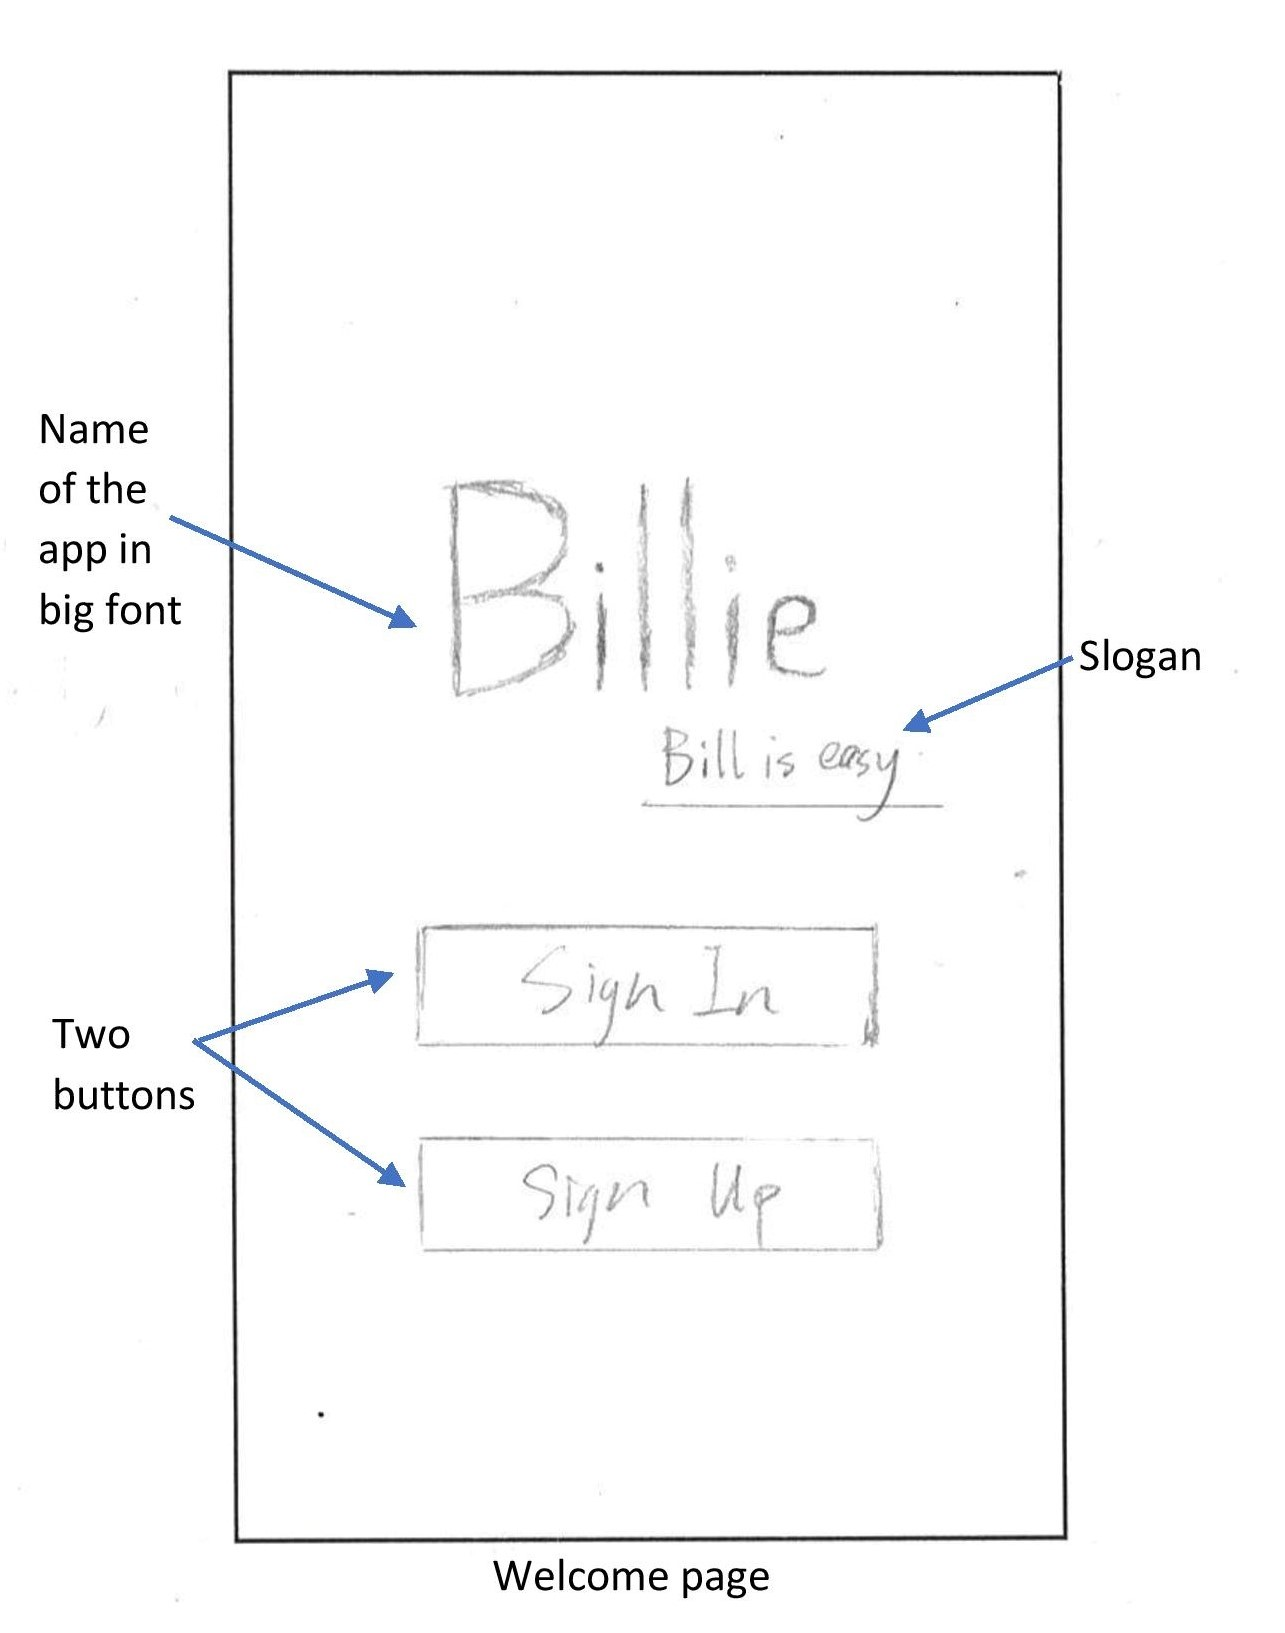
\includegraphics[width=0.6\columnwidth]{1-welcome-page.jpg}
  \caption{Sketch of welcome page for application Billie}
  \label{fig:figure16}
\end{figure}
As a user, I want to have my own account containing my personal bill information. The "Welcome" page, shown in Figure~\ref{fig:figure16}, consists of two options: "Sign in" or "Sign up". As a new user, I want to register an account. So the new user could tap on the "Sign up" button to go to the "Sign up" page shown in Figure~\ref{fig:figure17}.


\begin{figure}[h!]
\centering
  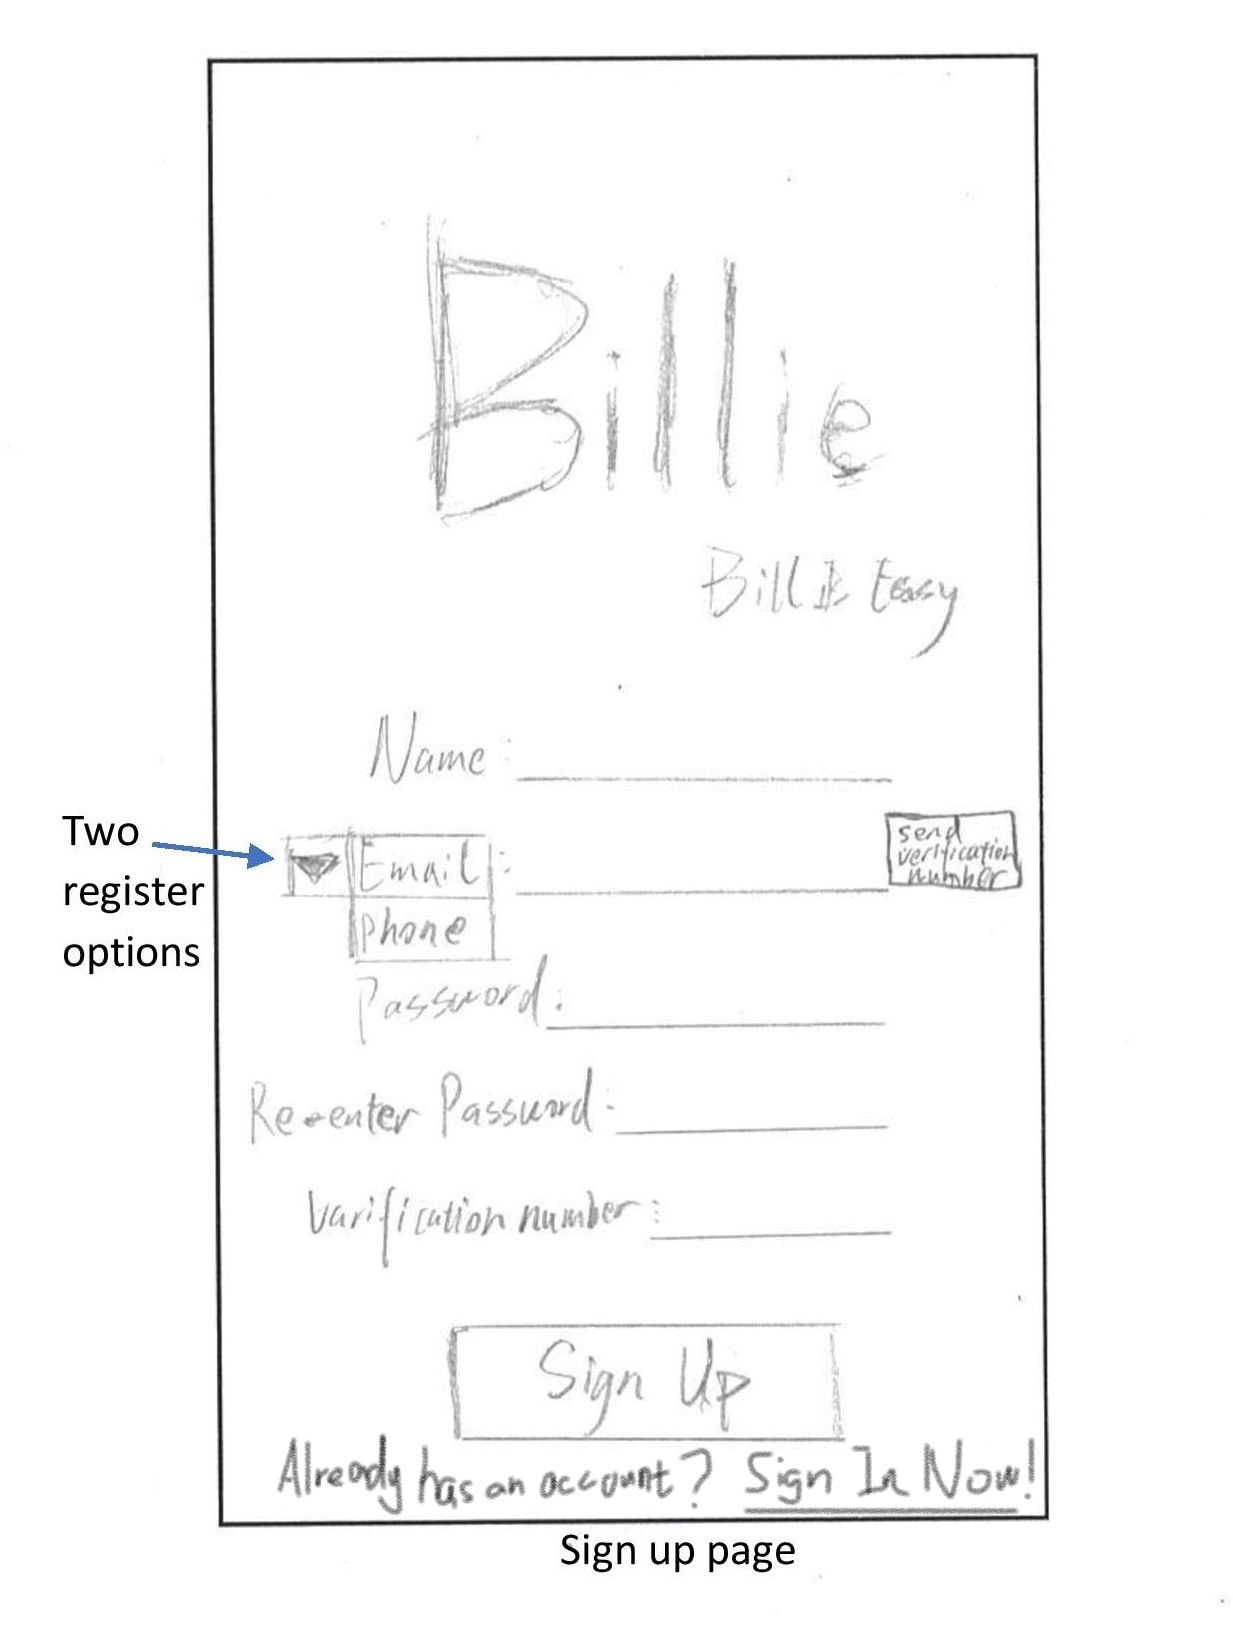
\includegraphics[width=0.6\columnwidth]{2-sign-up-page.jpg}
  \caption{Sketch of sign up page for application Billie}
  \label{fig:figure17}
\end{figure}
In the "Sign up" page, two options are provided for the user to sign up, by email or by phone number. The user would receive a verification number by one of the options selected. When all the information is correctly entered, the user can click sign up to create a personal account and to be redirected to the "Main/Home" page. If a registered user clicked the "Sign up" button by mistake, he/she has the option to be redirected back to the "Sign in" page by clicking the "Sign In Now" link located at the bottom of the screen.



\begin{figure}[h!]
\centering
  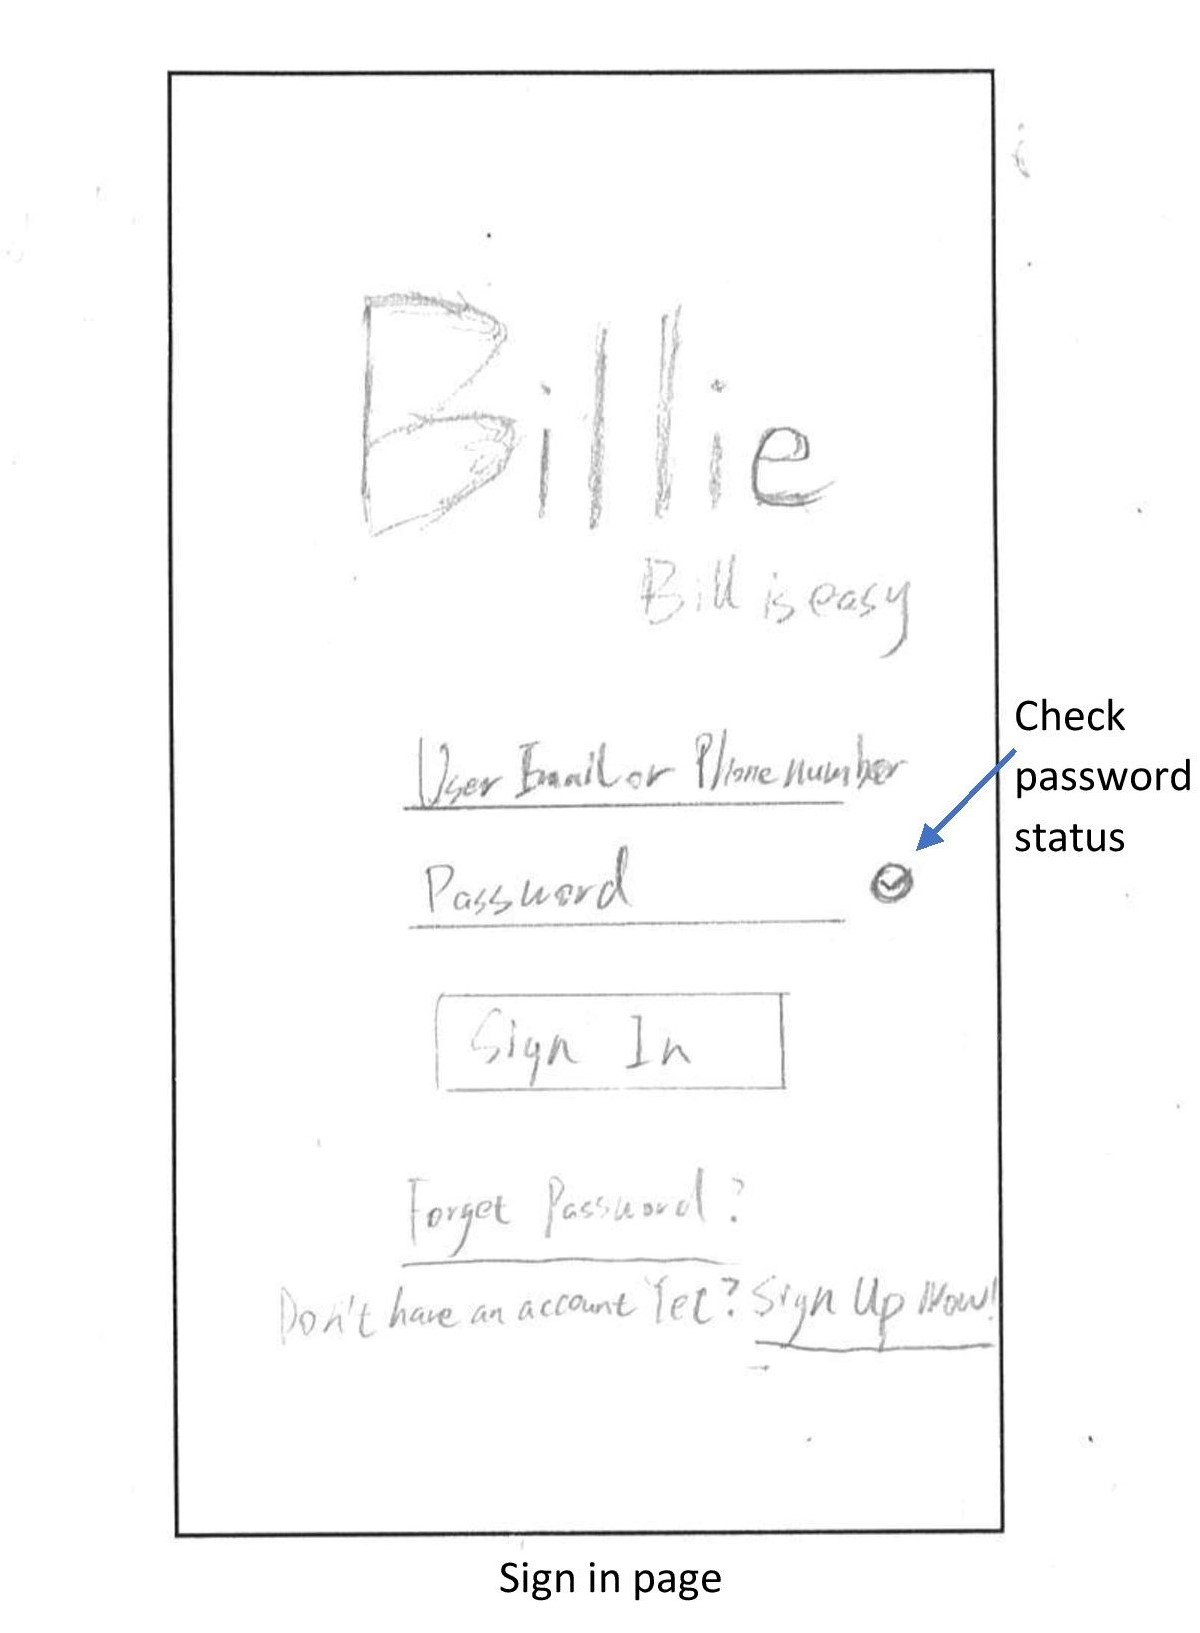
\includegraphics[width=0.6\columnwidth]{3-sign-in-page.jpg}
  \caption{Sketch of sign in page for application Billie}
  \label{fig:figure18}
\end{figure}
As a registered user, I want to sign in to my account. One can simply tap on the "Sign in" button on the "Welcome" page to go to the "Sign in" page shown in Figure~\ref{fig:figure18}. The user can type in the user email or phone number and password to sign in to their Billie account. A small grey password check icon is located on the right of the password entry for the user to see if they entered the password correctly. As a user, I want to reset my password if I forget it, so that I don't lose my account forever. Therefore, a "Forget Password" option is provided for the user to enter their credentials for receiving a password reset link. If a new user clicks the "Sign in" button by mistake, he/she has the option to be redirected back to the "Sign up" page by clicking the "Sign Up Now" link. If everything is correctly entered, the user can tap on the "Sign In" button to be redirected to the "Main/Home" page.



\begin{figure}[h!]
\centering
  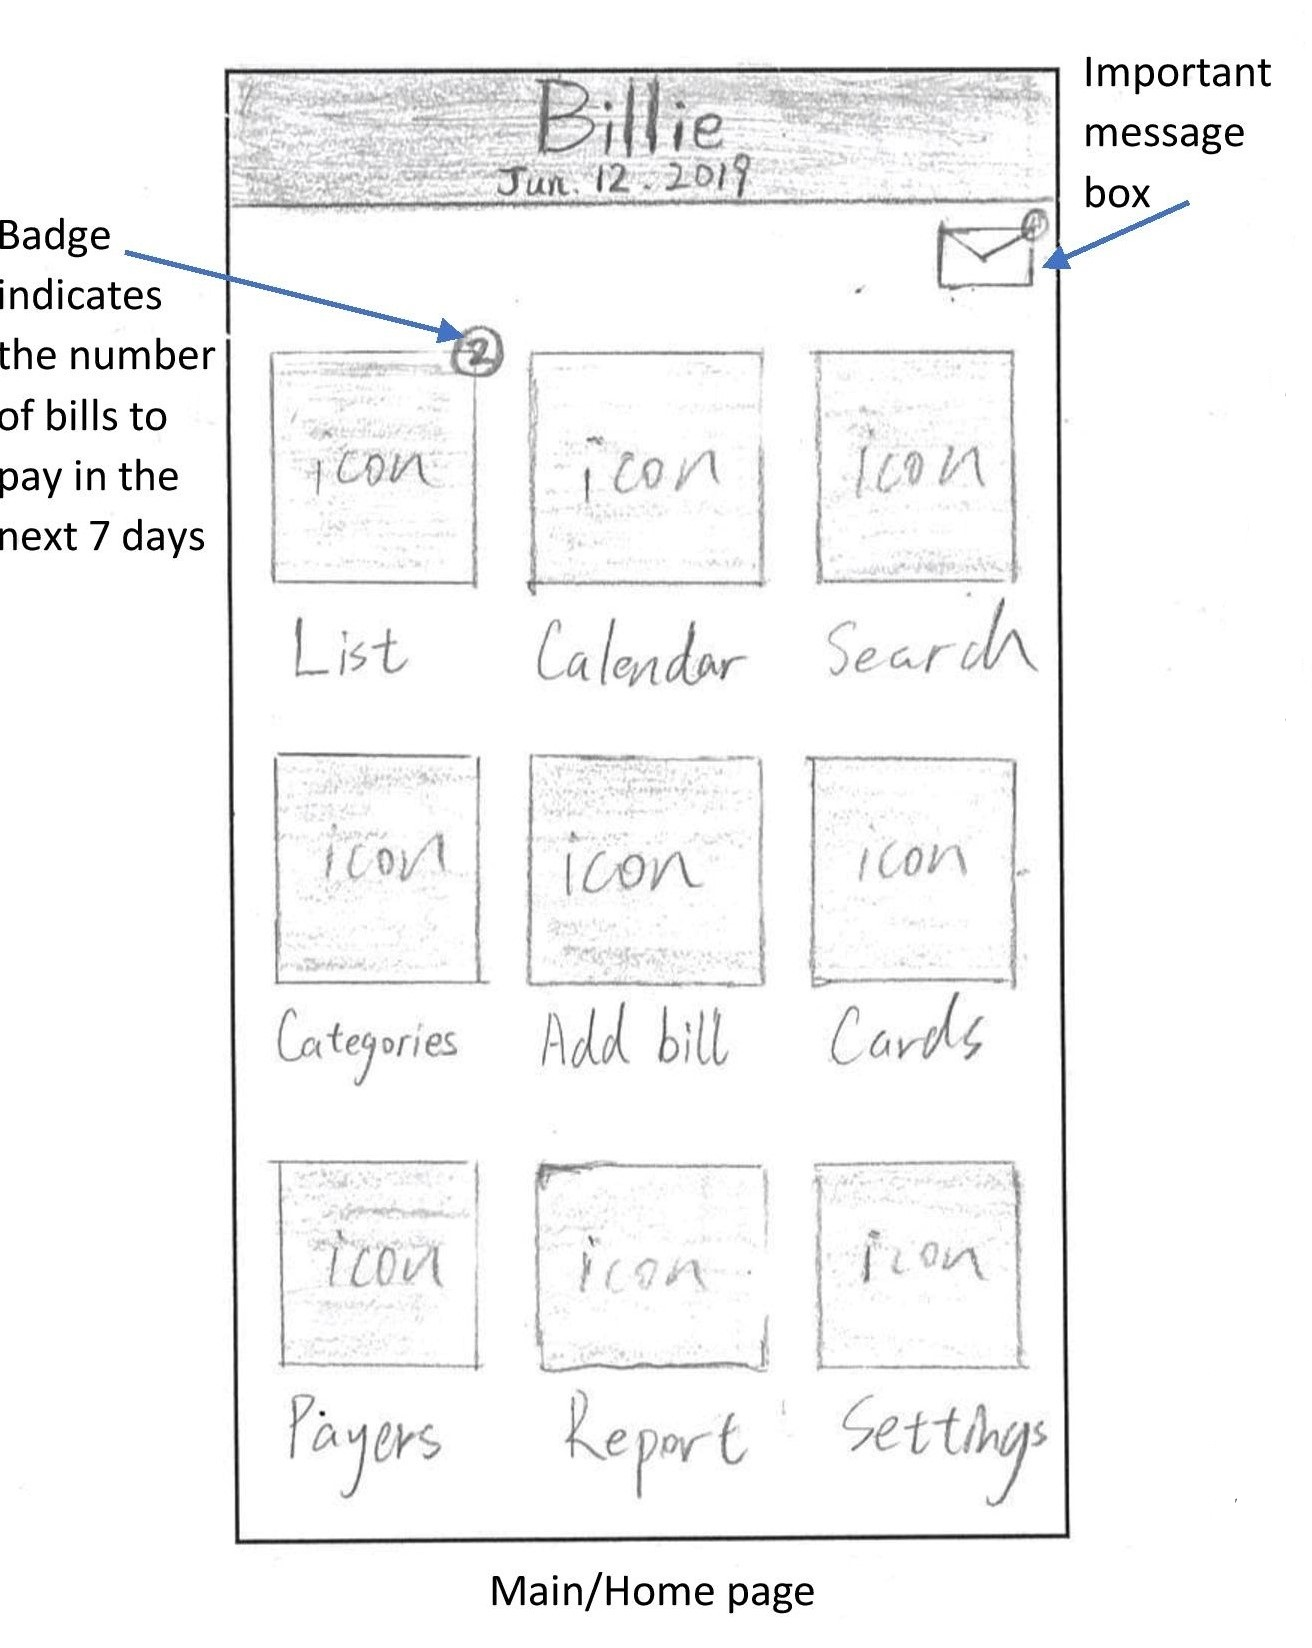
\includegraphics[width=0.6\columnwidth]{4-main-home-page.jpg}
  \caption{Sketch of main/home page for application Billie}
  \label{fig:figure19}
\end{figure}
On the "Main/Home" page, as shown in Figure ~\ref{fig:figure19}, the user can see all features at a glance. Nine square-shaped icons, each with a specific goal, are placed evenly across the middle of the screen in a 3 by 3 grid. On the top right corner, there is a small envelope icon, different from all other icons, indicating the important message box, which will be introduced later. The 9 icons are "List", "Calendar", "Search", "Categories", "Add bill", "Cards", "Pages", "Report", "Settings". The users can tap on an icon to go perform the corresponding task. Let's explore the "Settings" page first by tapping on the "Settings" icon.



\begin{figure}[h!]
\centering
  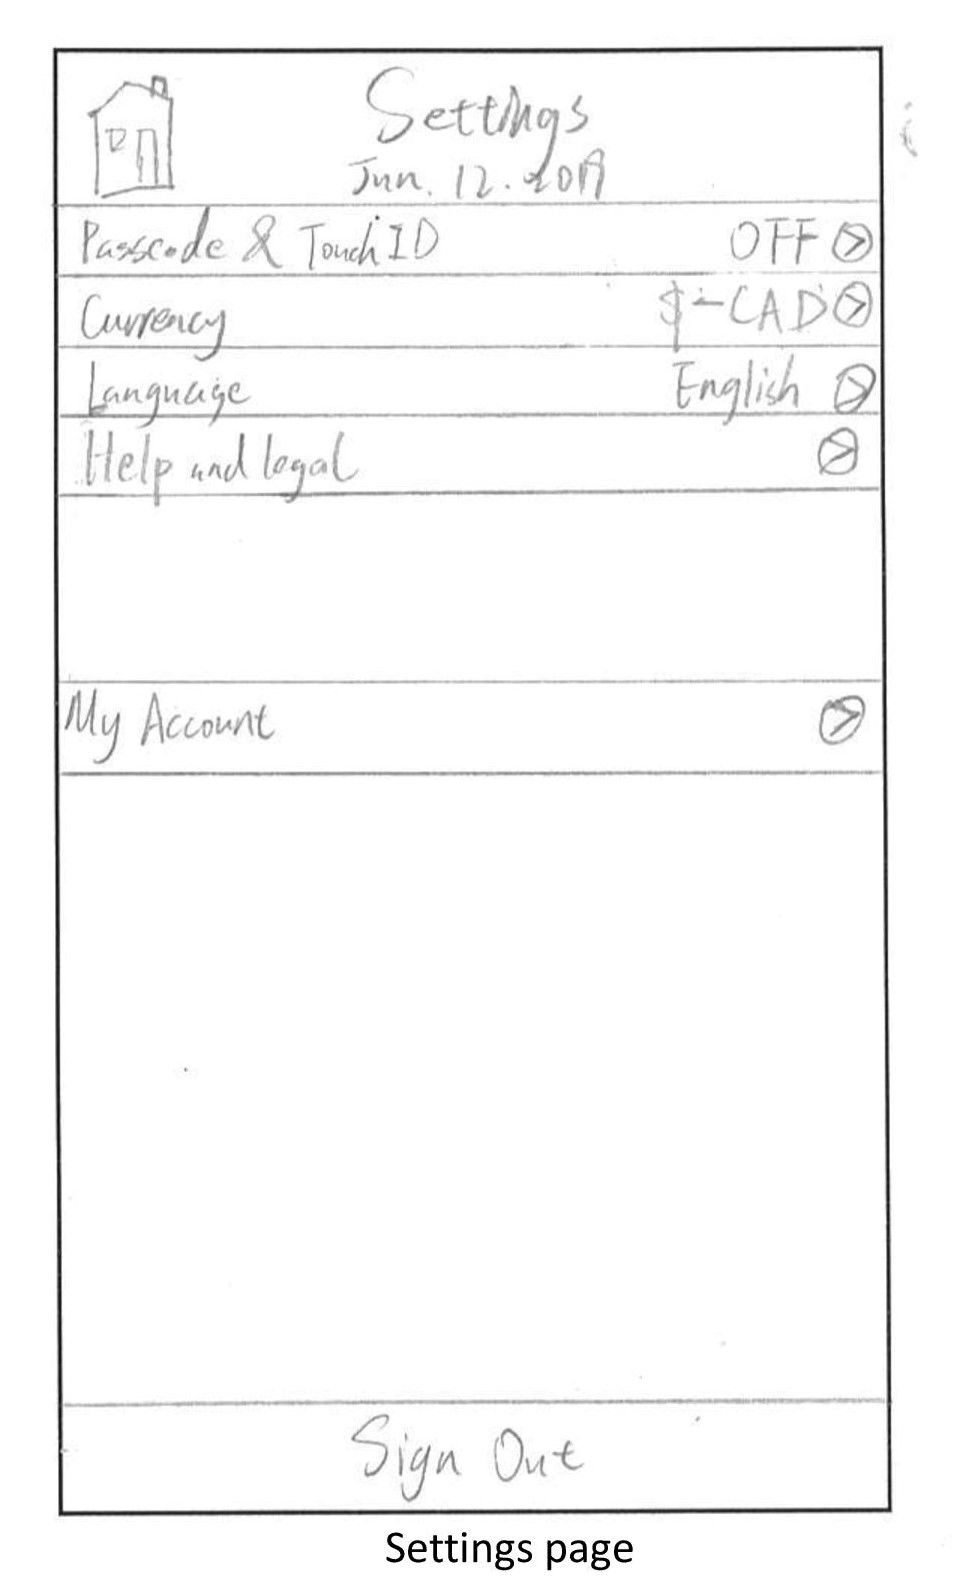
\includegraphics[width=0.5\columnwidth]{5-settings-page.jpg}
  \caption{Sketch of settings page for application Billie}
  \label{fig:figure20}
\end{figure}
As a user, I want to adjust the settings, so that I can configure the application based on my preference. In the "Settings" page shown in Figure~\ref{fig:figure20}, the user can adjust options such as language, currency, and PIN, etc. The user can also click the "Sign Out" button located on the bottom of this page to sign out of the account. The little home icon on the top left corner on all pages will bring the user back to the "Main/Home" page. To add on another level of security, the user can turn on the fingerprint or facial identification toggle to link the on-device biometric authentication method to the account. Now, suppose the user closed Billie or put it in the background.




\begin{figure}[h!]
\centering
  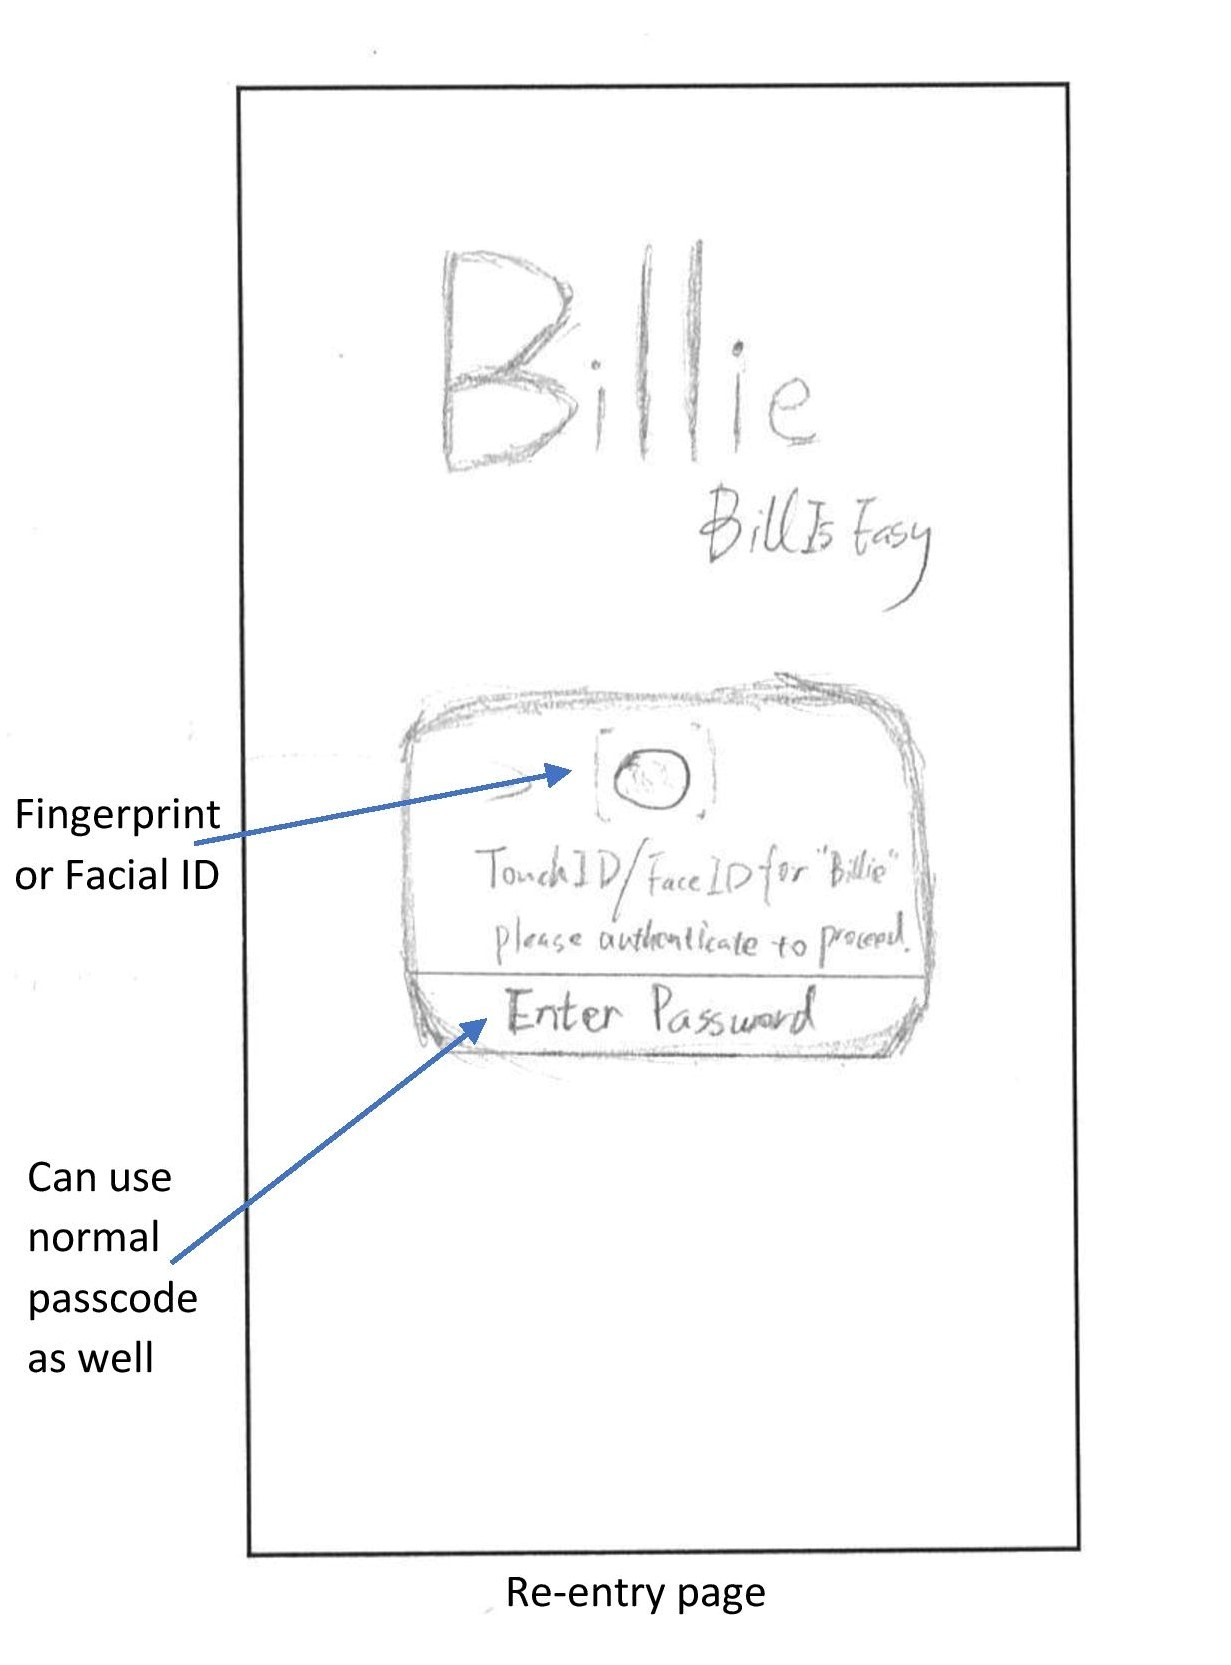
\includegraphics[width=0.6\columnwidth]{6-re-entry-page.jpg}
  \caption{Sketch of re-entry page for application Billie}
  \label{fig:figure21}
\end{figure}
The re-entry identification page, shown in Figure~\ref{fig:figure21}, shows up every time Billie is started up or brought back from the background under logged in status. A re-entry authentication is required using the modern on-device biometric authentication methods such as fingerprint or facial identification for easier login process. If the two methods are not available, a PIN option is also provided. All these levels of authentication implementations should address the privacy and security concerns one would have using a personal finance related application and give the users the confidence to save their important information safely within Billie.



\begin{figure}[h!]
\centering
  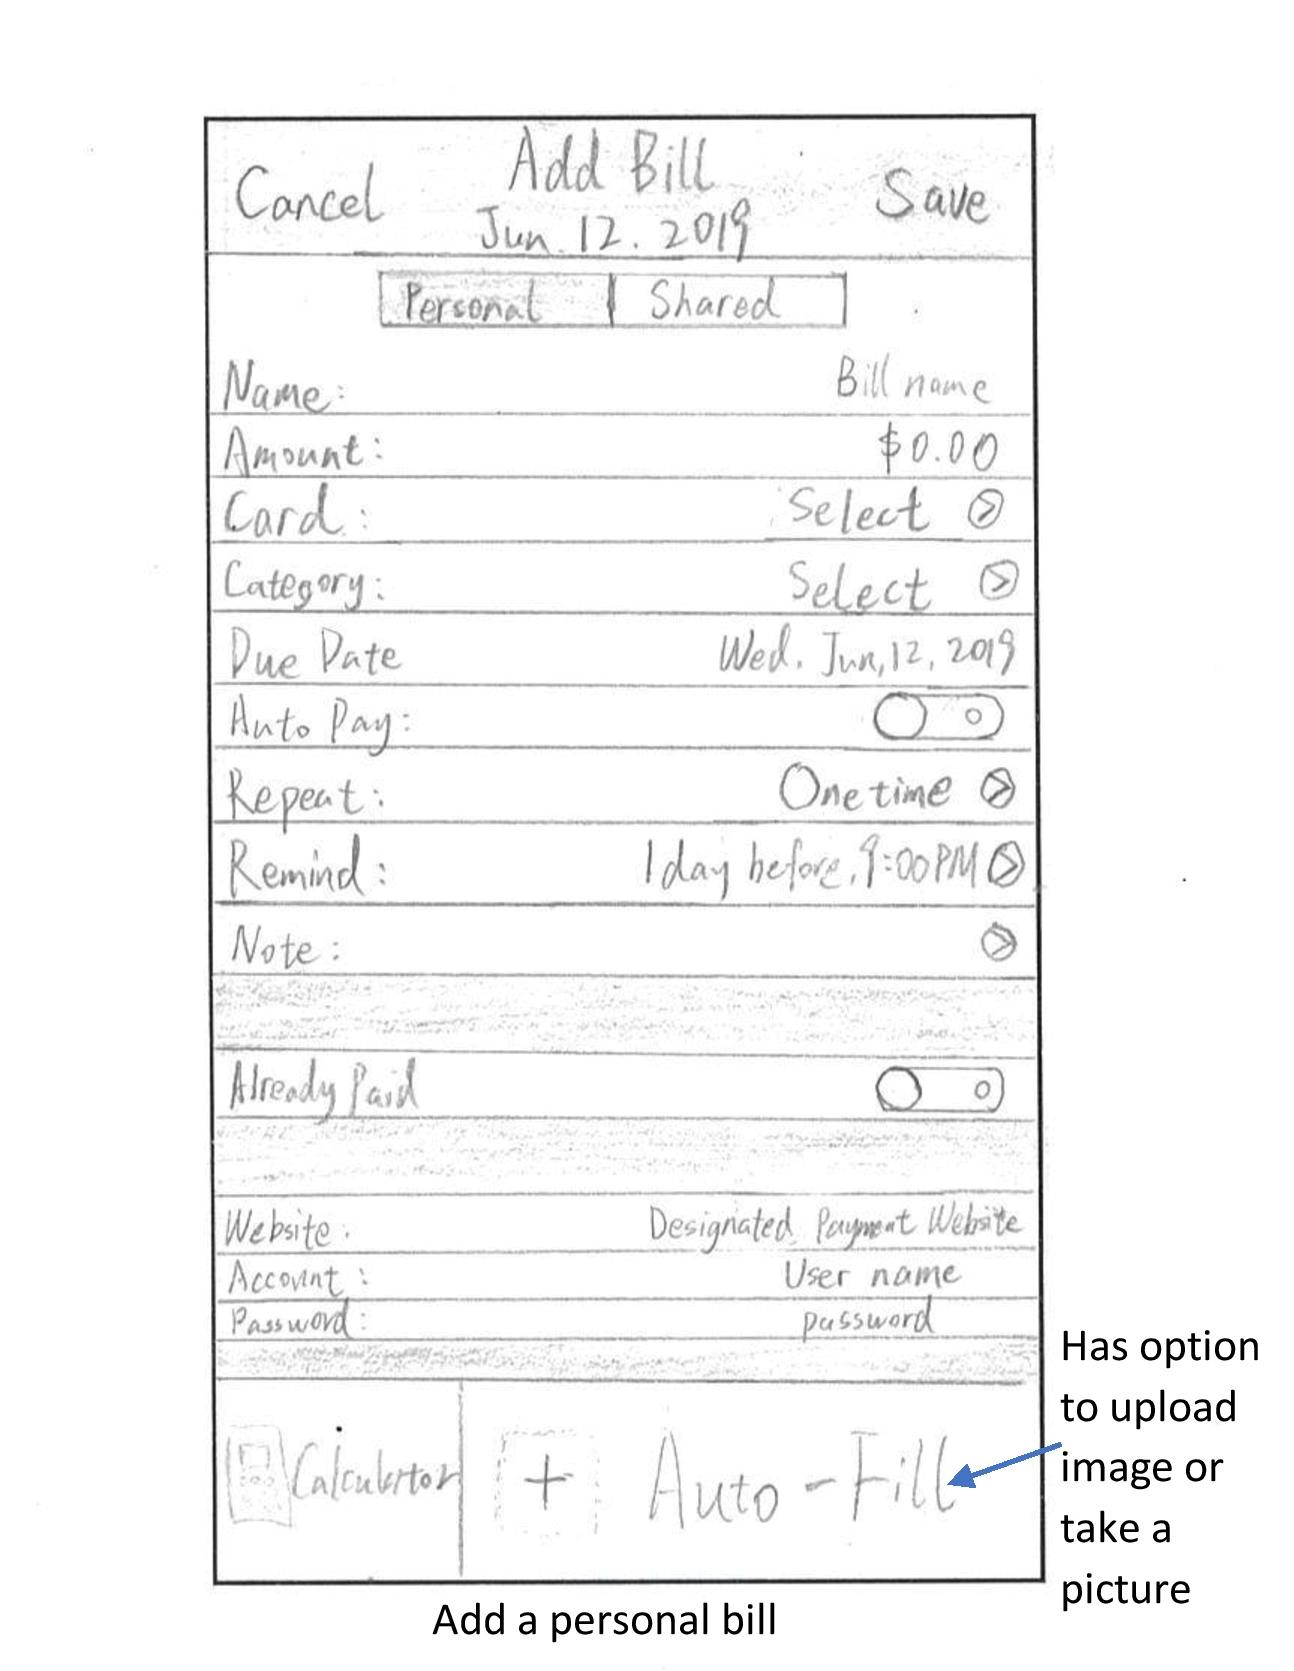
\includegraphics[width=0.6\columnwidth]{7-add-bill-page.jpg}
  \caption{Sketch of add personal bill page for application Billie}
  \label{fig:figure22}
\end{figure}
\begin{figure}[h!]
\centering
  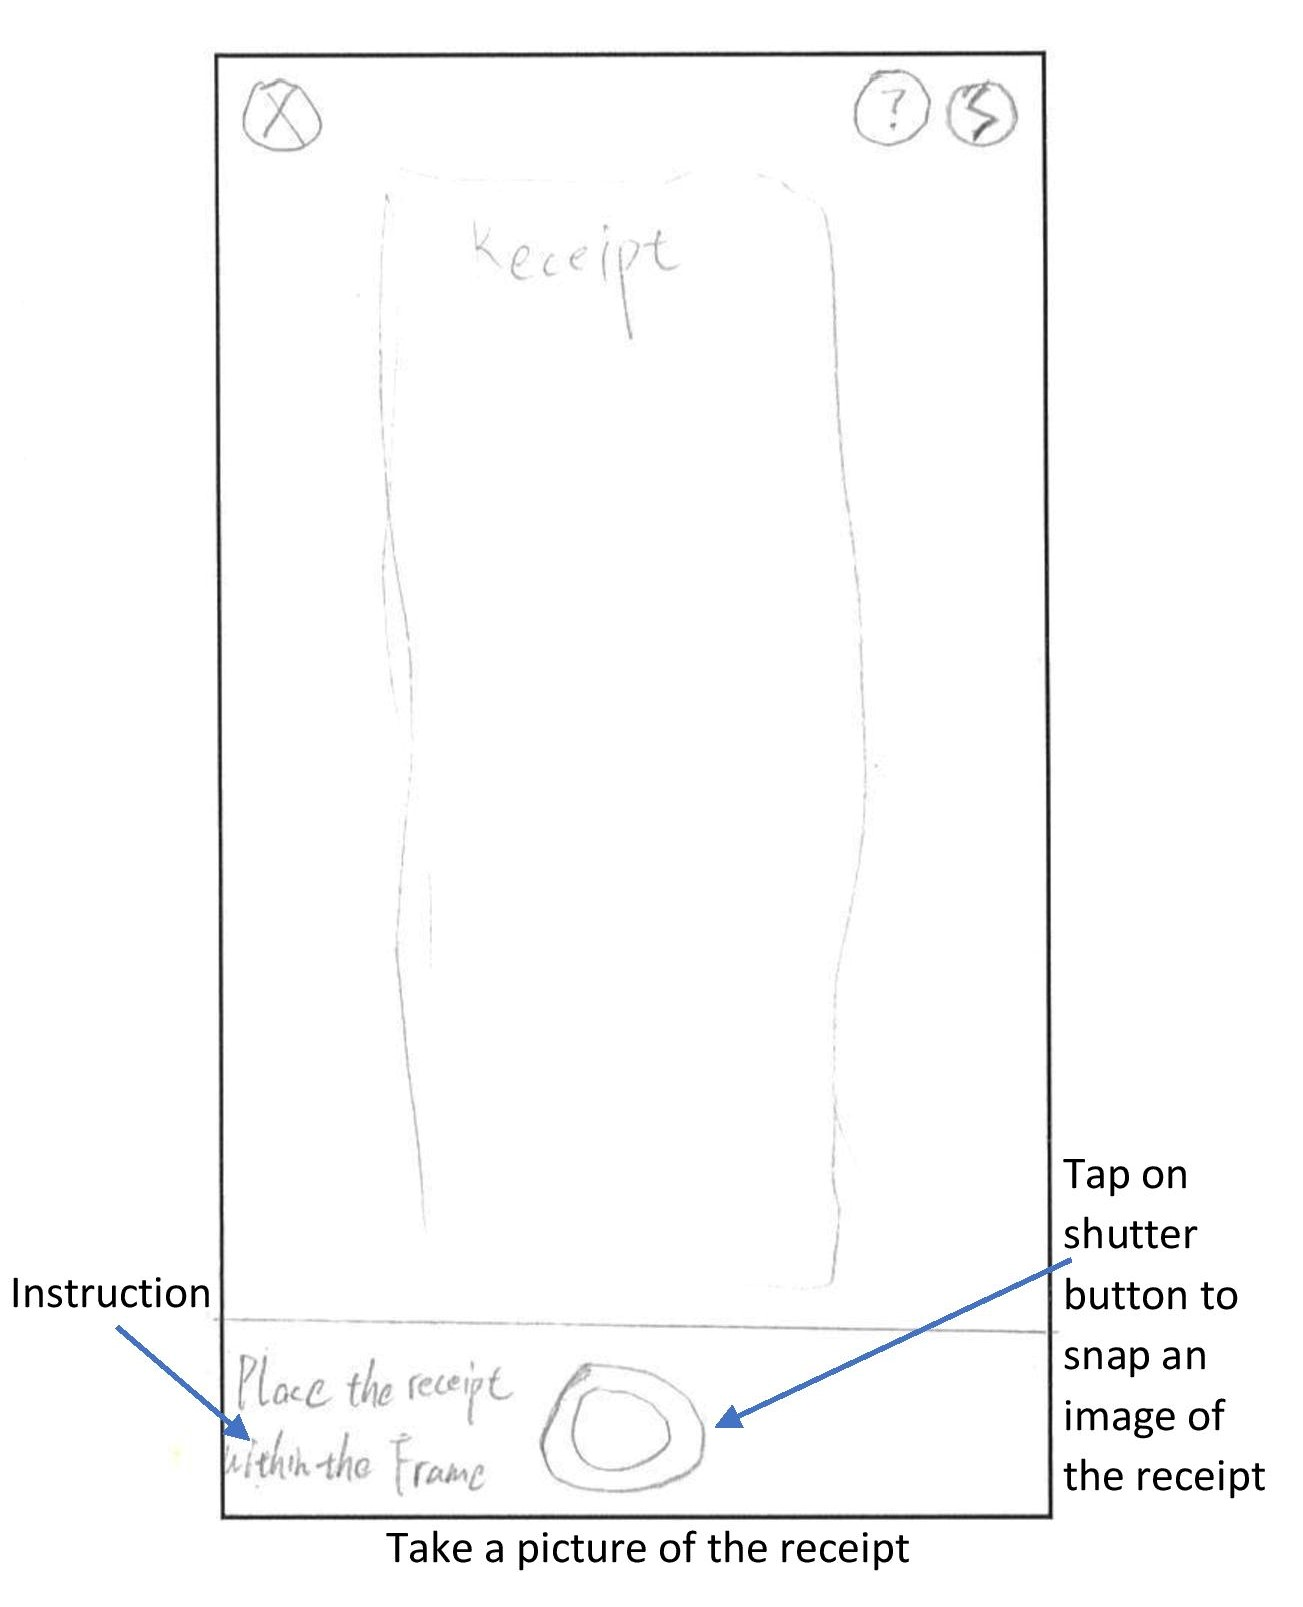
\includegraphics[width=0.6\columnwidth]{8-scan-image-page.jpg}
  \caption{Sketch of scan receipt page for application Billie}
  \label{fig:figure23}
\end{figure}
As a user, I want to add bills, so that I can keep track of them. Therefore, as a bill management application, the most important feature would be to "Add bill", which is the central icon placed in the "Main/Home" page. By tapping on that icon, the user will go to an "Add bill" page. The bills are categorized into two types: personal bills and shared bills. The user can switch between "Personal" and "Shared" by tapping on the corresponding tab. Each personal bill has some properties, as shown in Figure ~\ref{fig:figure22}, that need to be filled in. The reminder date is highly adjustable and can be set to be in repeat ever given periods. As a user, I want to see my online payment website, account, and password associated with a bill, so that I don't need to go search elsewhere. Online payment information such as website, account, and password can be saved optionally for easier in-app access. As a user, sometimes I don't want to manually type in all this information. An "Auto-Fill" option is provided on the bottom of the page so that the user has the option to upload an image or take a picture of the receipt, as shown in Figure ~\ref{fig:figure23}.

\begin{figure}[h!]
\centering
  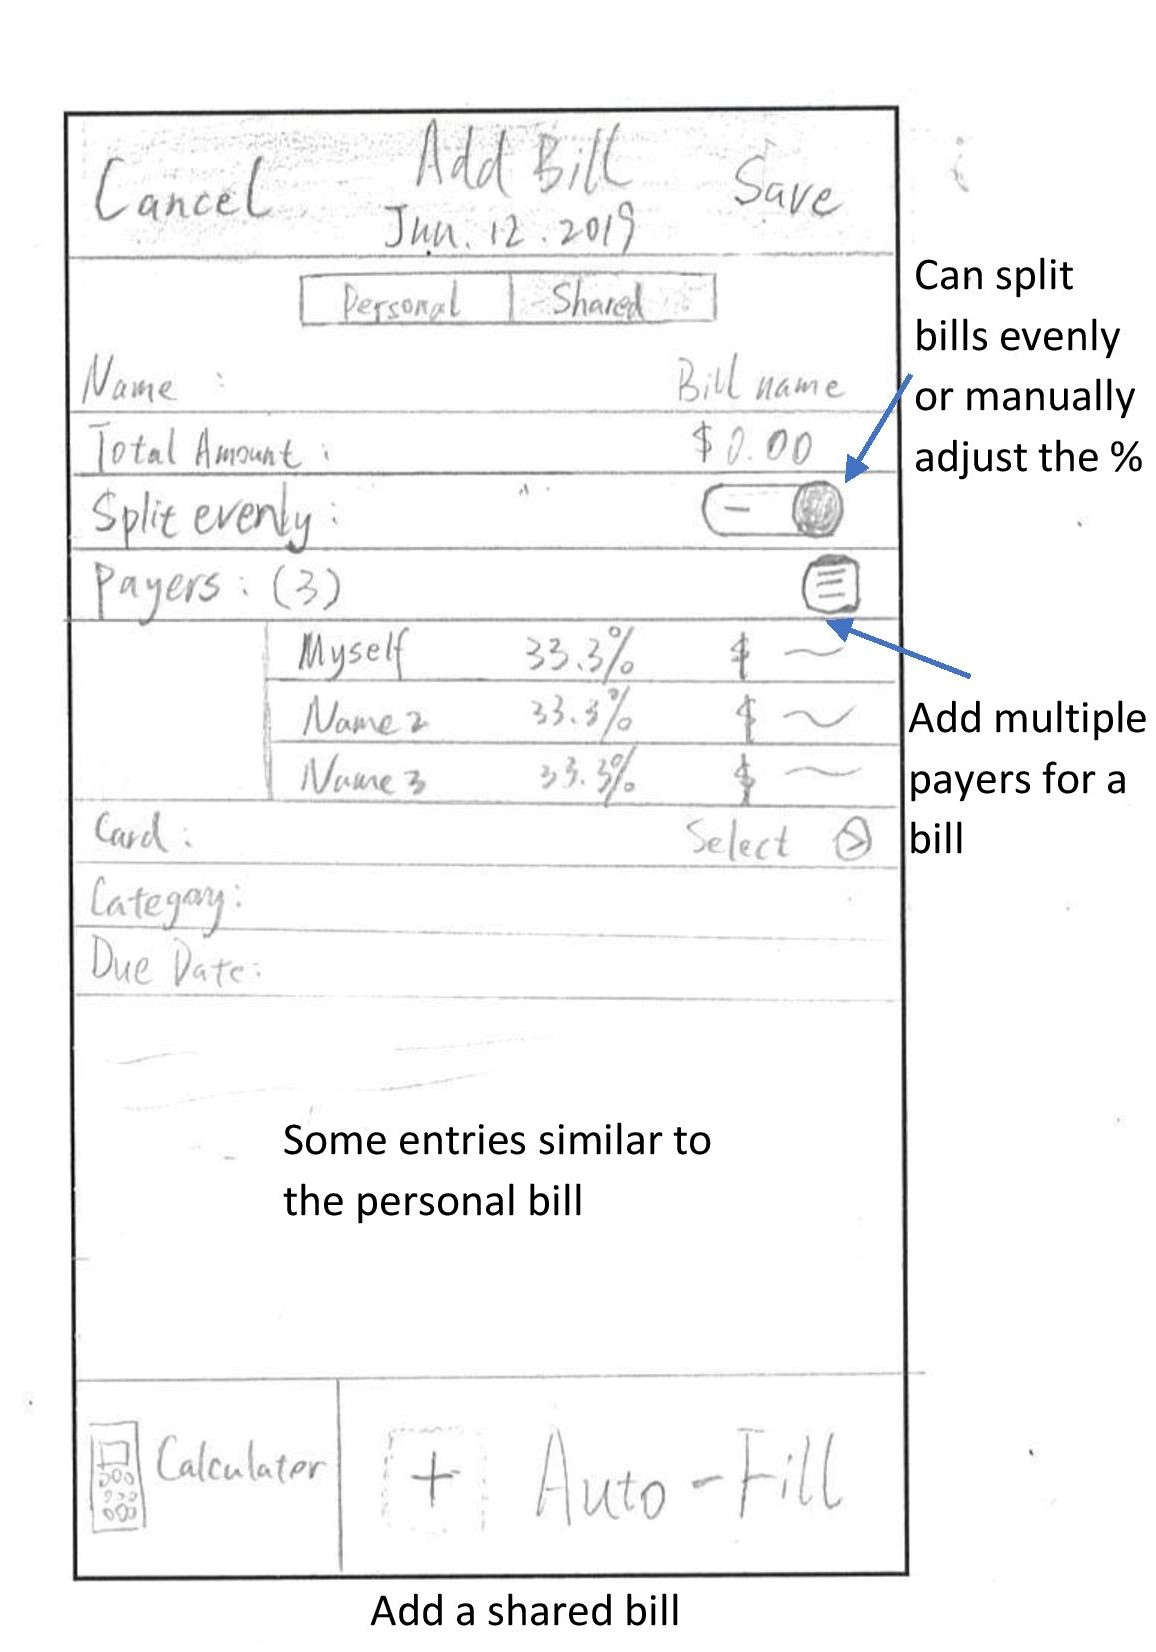
\includegraphics[width=0.6\columnwidth]{9-add-shared-bill-page.jpg}
  \caption{Sketch of add shared bill page for application Billie}
  \label{fig:figure24}
\end{figure}

As a user, I want all co-payers of a bill be notified, so that I don't need to remind them of it. As shown in Figure~\ref{fig:figure24}, the user can click on the "Shared" tab in the "Add bill" page to create a shared bill that will be synchronized across all associate payers. The creator of the bill can select multiple payers from the "Payers" page by clicking on the small icon. The user can split the bills evenly or manually adjust the percentage for all payers. It is expected that not all co-payer uses Billie, then the notification and updates will be sent out through email or message. The co-payer of the bill needs to accept to be enrolled in a particular bill.



\begin{figure}[h!]
\centering
  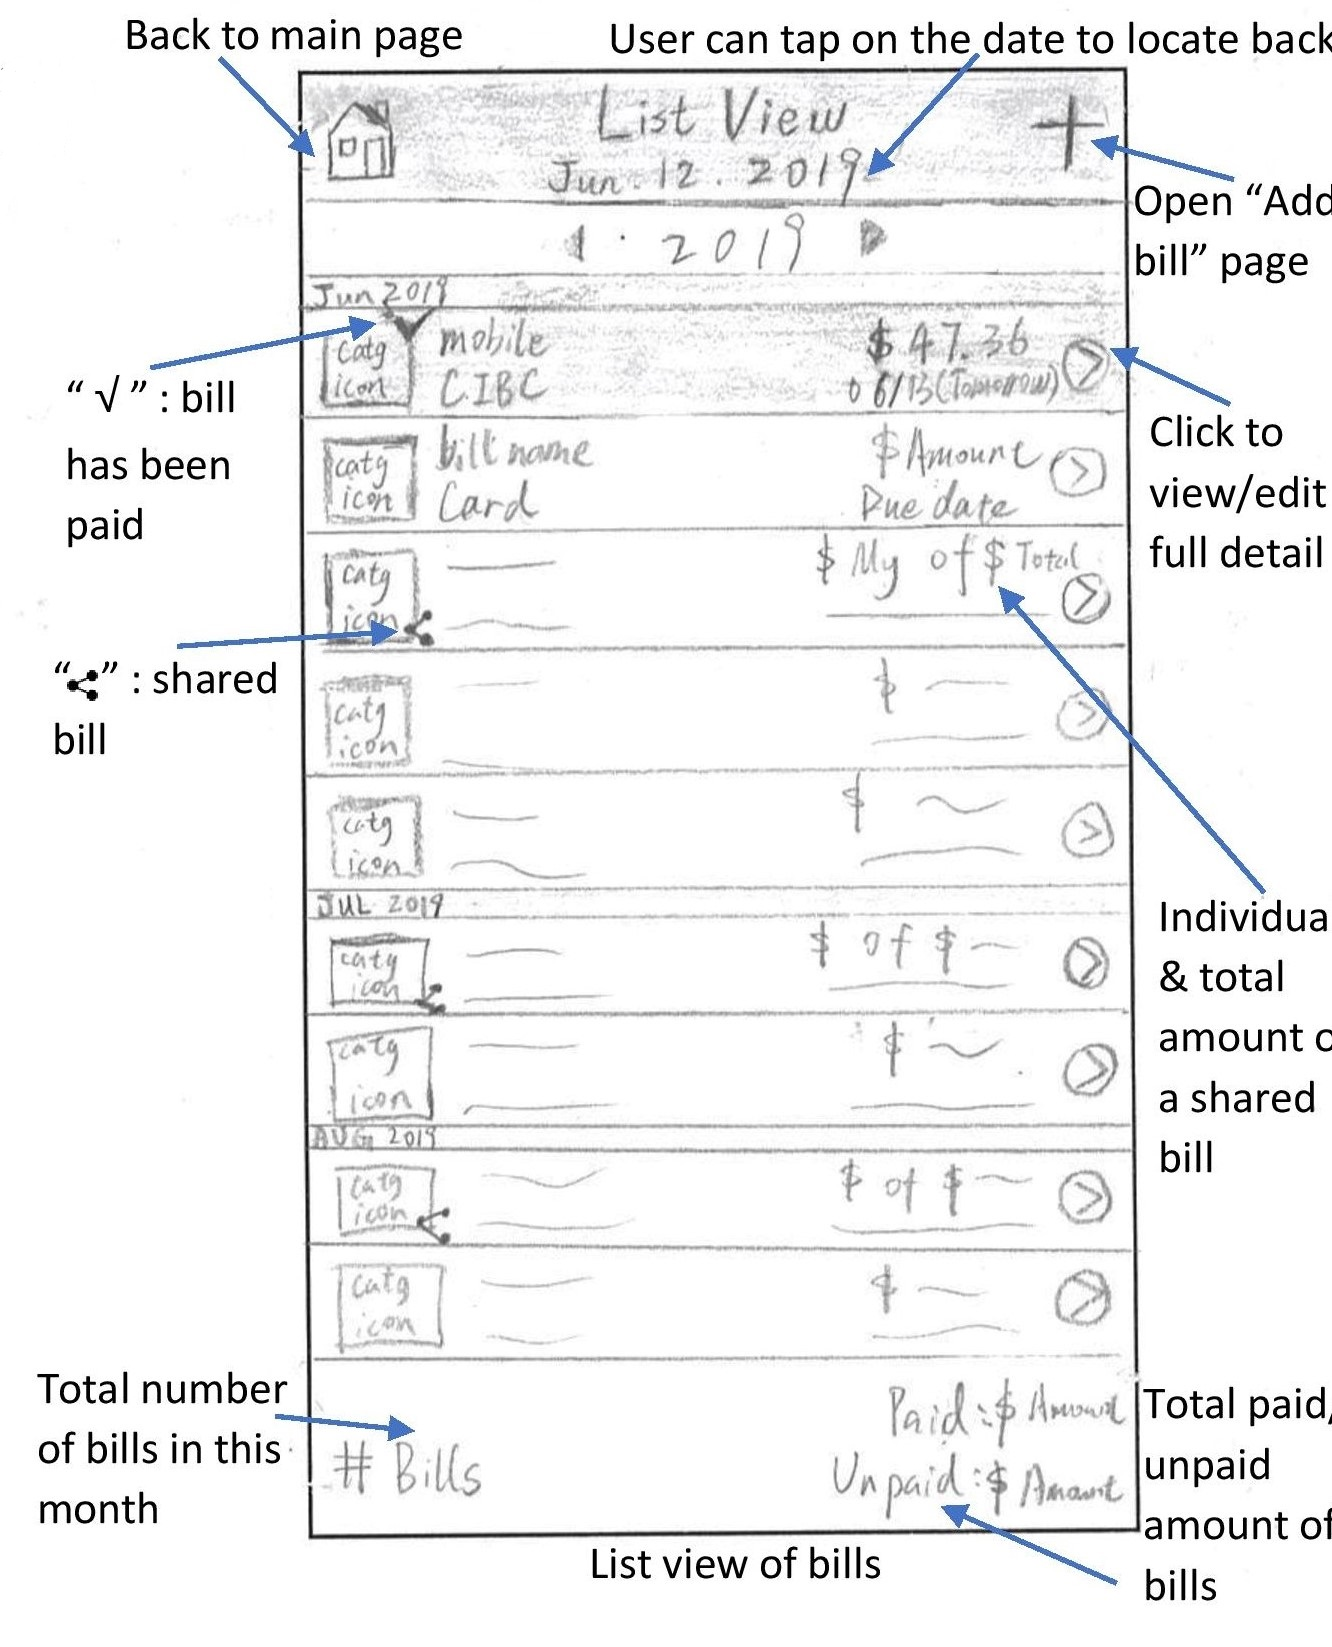
\includegraphics[width=0.6\columnwidth]{10-list-view-page.jpg}
  \caption{Sketch of list view of bills page for application Billie}
  \label{fig:figure25}
\end{figure}
Now, as a user, I need to view all my saved bills. On the "Main/Home page", the user can click either "List" icon or "Calendar" icon to view saved bills in list or calendar views. Suppose the user taps on the "List" icon, "List view" page, shown in Figure~\ref{fig:figure25}, shows all the saved bills in the current calendar year in a list. Each bill is an individual entry and is arranged in chronological order. By default, the top entry will be the bill closest to date. The user can scroll down to view the previous bills. The user can tap on the current date on the banner if he/she wants to relocate back to the most recent bill. Tapping on the left and right arrow of the year can bring you to the list view of bills in previous or next calendar year. Major details of a bill, such as category, name, card, amount, due date and payment status, etc, are displayed in a fixed format on each entry for quick access. Tapping on the icon on the right of each bill entry will bring you to view or edit a bill detail. A summary bar on the bottom shows some analysis of bills in a month. The user can add a new bill by tapping on the "+" icon on the top right corner, which would open the "Add bill" page. Now suppose the user clicks back to the main page and tap on the "Calendar" icon.



\begin{figure}[h!]
\centering
  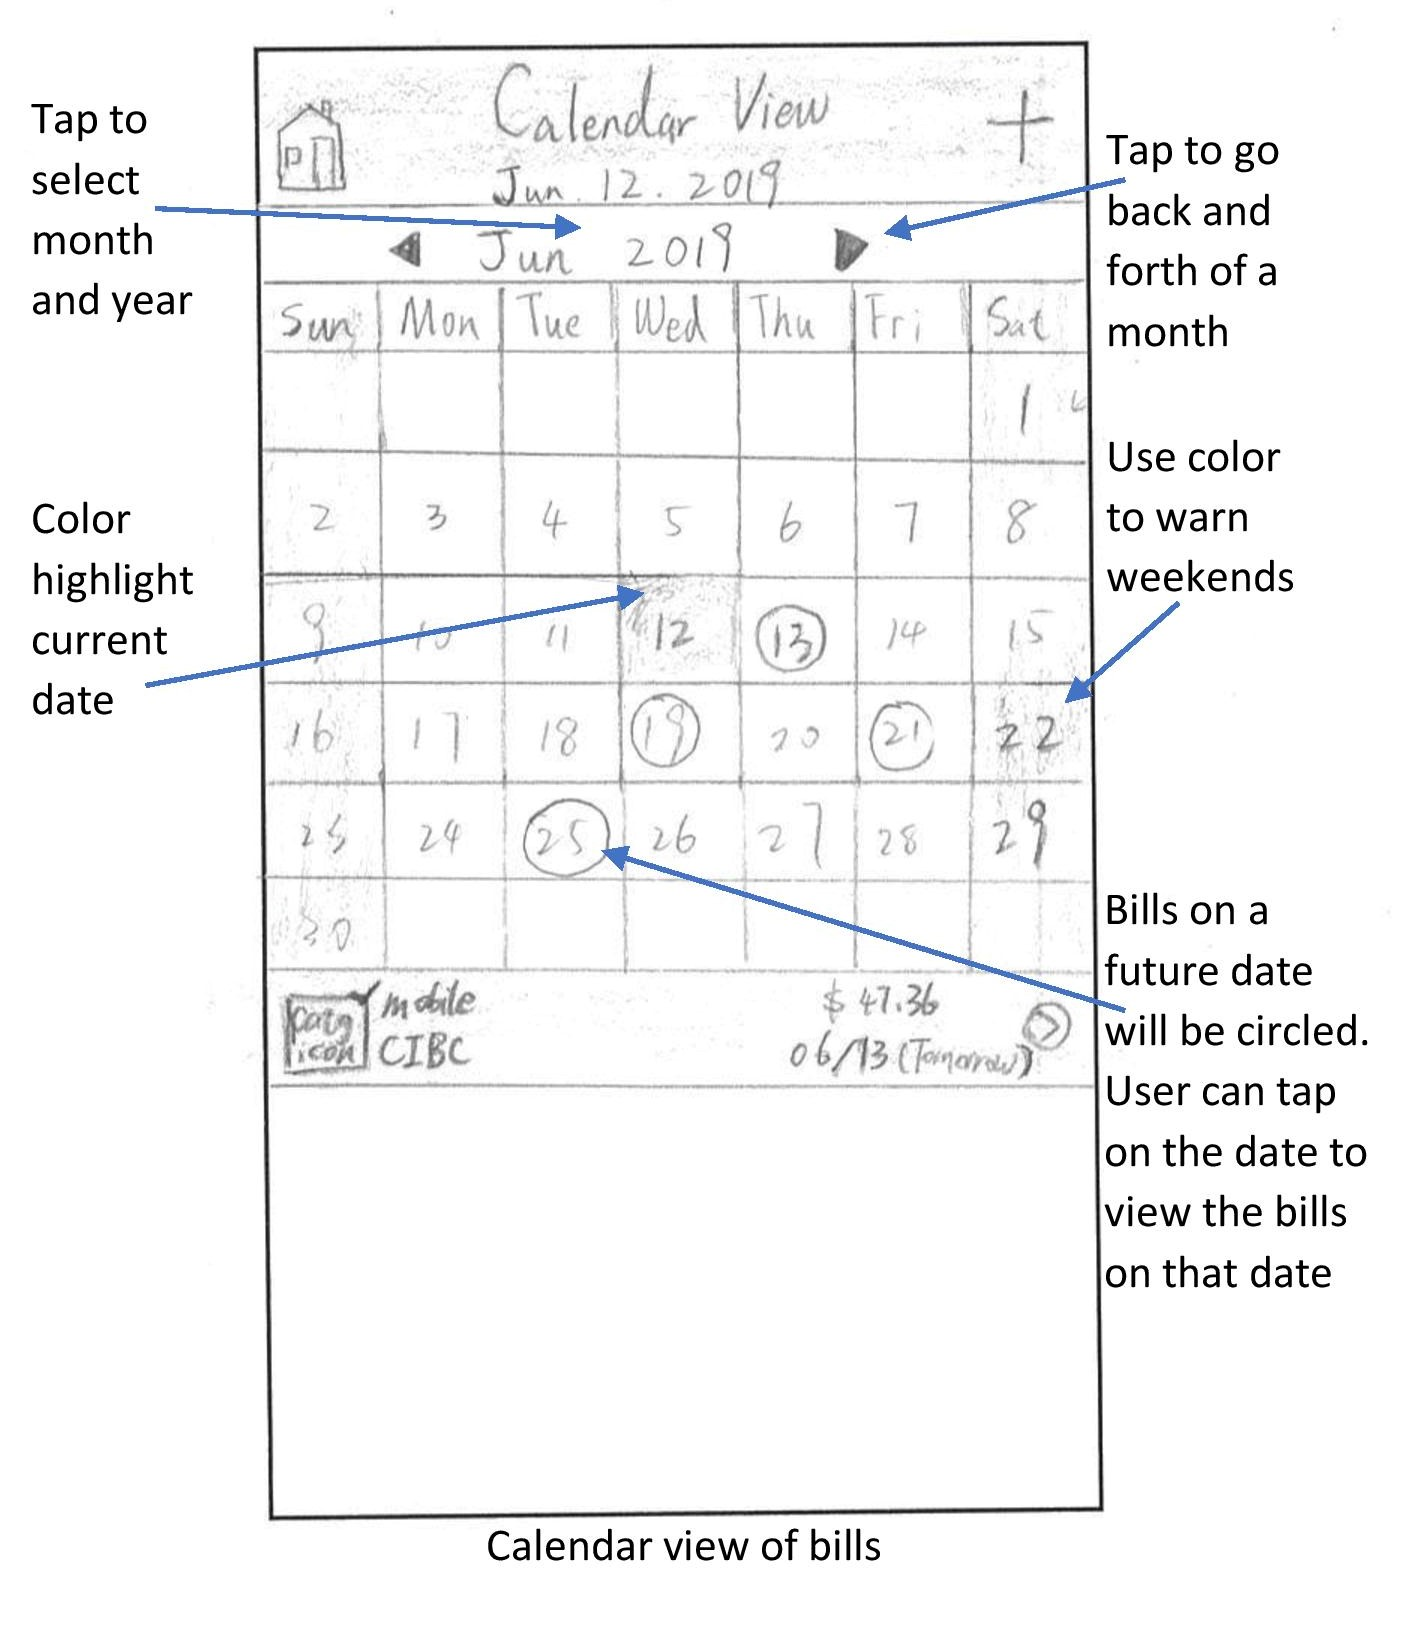
\includegraphics[width=0.6\columnwidth]{11-calendar-view-page.jpg}
  \caption{Sketch of calendar view of bills page for application Billie}
  \label{fig:figure26}
\end{figure}
The "Calendar view" page, as shown in Figure~\ref{fig:figure26}, provides the user with another convenient way of viewing their saved bills. All upcoming bill dates are marked with circles. The user can tap on the date to view the bills on that date. The calendar is in month view and the user can tap to change the month and years. Other functionalities are similar to the ones in the "List view" page. 


\begin{figure}[h!]
\centering
  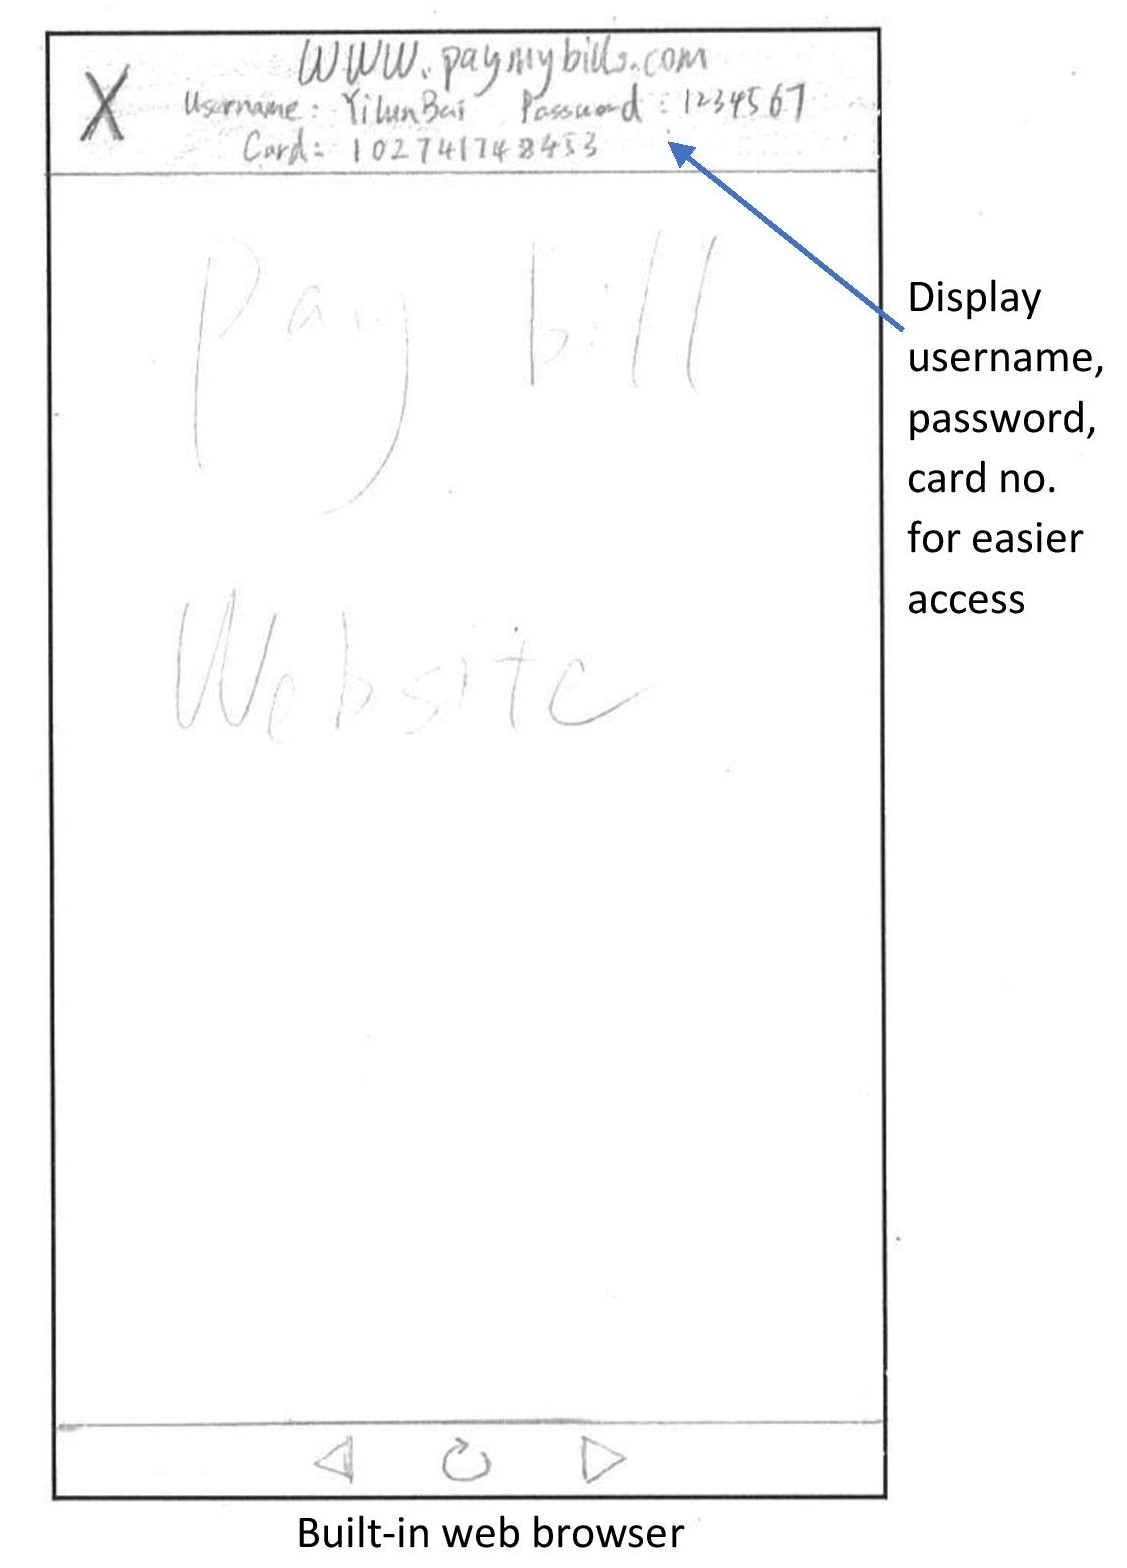
\includegraphics[width=0.6\columnwidth]{12-web-browser-page.jpg}
  \caption{Sketch of built-in web browser page for application Billie}
  \label{fig:figure27}
\end{figure}
As a user, I want to pay my bill directly within the application, so that I don't need to open an external browser. As shown in Figure~\ref{fig:figure27}, by tapping the website saved in a bill, the built-in browser will load the web-page, and display useful information for users, such as username, password, and card number, to improve the convenience of bill payments.


\begin{figure}[h!]
\centering
  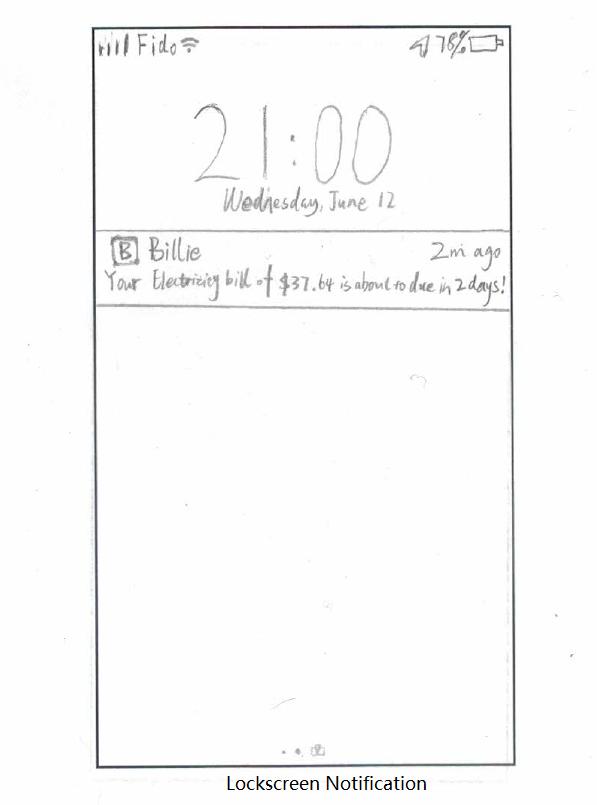
\includegraphics[width=0.6\columnwidth]{13-notification.png}
  \caption{Sketch of lock-screen notification for application Billie}
  \label{fig:figure28}
\end{figure}
\begin{figure}[h!]
\centering
  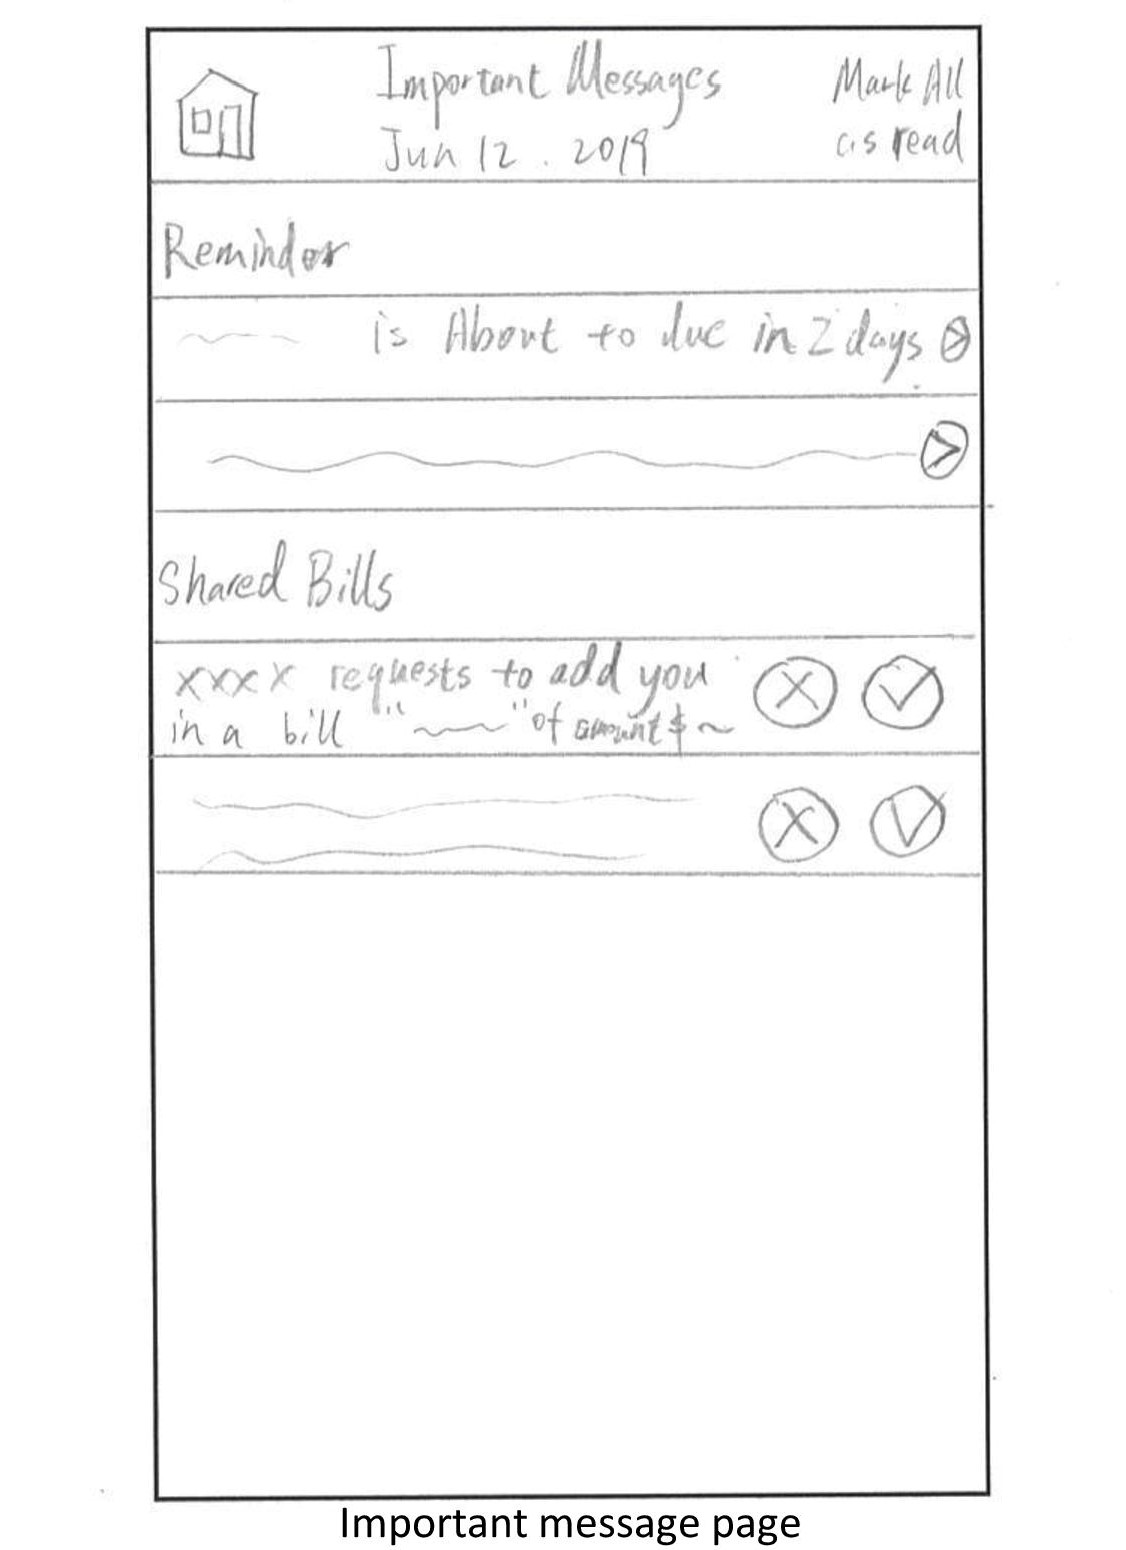
\includegraphics[width=0.6\columnwidth]{14-important-message-page.jpg}
  \caption{Sketch of important message page for application Billie}
  \label{fig:figure29}
\end{figure}
As a user, I want to be notified when a due date is approaching, so that I won't miss the deadline. I also want to be notified when someone added me to a shared bill, so that I can examine it. Figure~\ref{fig:figure28} shows a bill notification from Billie on the lock screen. The user can easily see the bill that is about to pass the due date. From the "Main/Home" page of the app, a badge of the number of unread messages is shown on the top right corner of the envelope icon. The "Important message" page, as shown in Figure~\ref{fig:figure29}, can be accessed by tapping on the little envelope icon or by tapping on the notification. There are two kinds of important messages: one is the reminders for upcoming bills, the other is when someone added you as a payer for a shared bill. A user can confirm or decline a shared bill request by tapping either the "X" or "\checkmark". By accepting the shared bill, the bill will be added to the account. A user can tap on the reminder message to view the important bill that is approaching the deadline and change the status.



\begin{figure}[h!]
\centering
  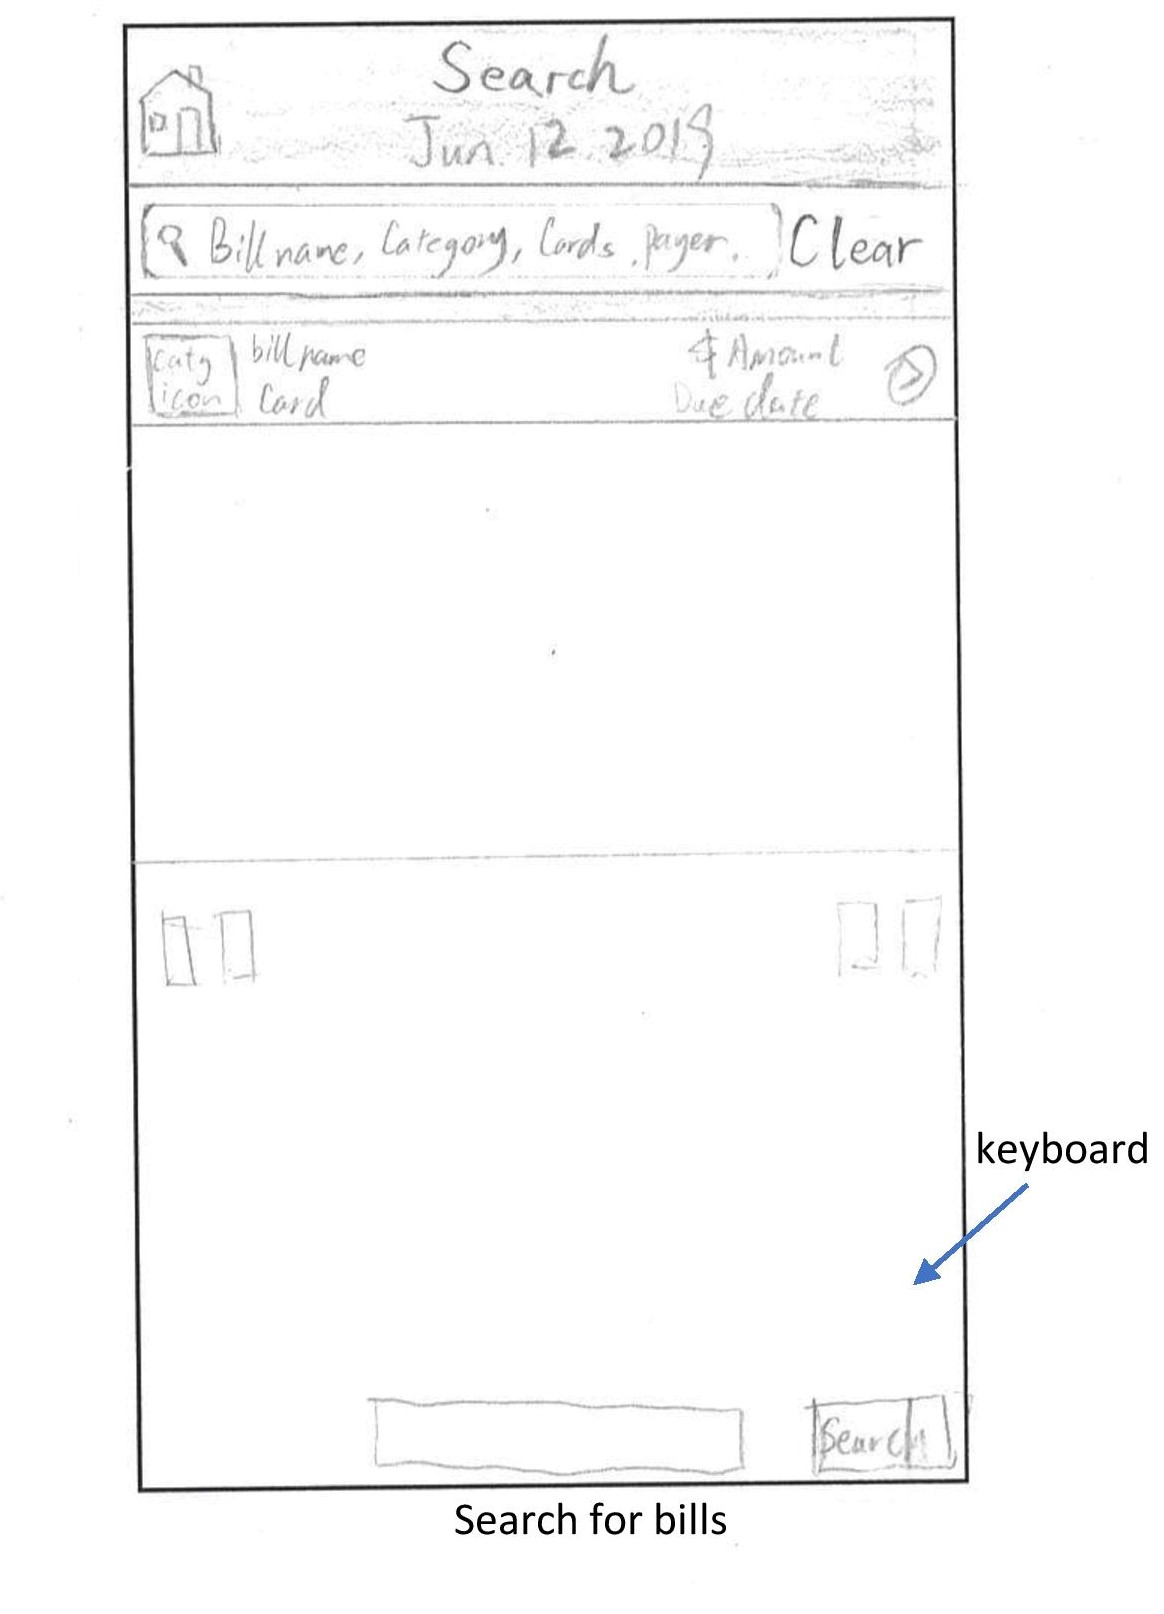
\includegraphics[width=0.6\columnwidth]{15-search-bill-page.jpg}
  \caption{Sketch of search page for application Billie}
  \label{fig:figure30}
\end{figure}
As a user, I want to search for bills, so that I find bills with certain properties as I need. On the "Main/Home" page, the user can tap on the "Search" icon to go to the "Search" page as shown in Figure~\ref{fig:figure30}. A search bar is presented with a prompt for search terms such as "Bill name, category, cards, payer ...". If the user wants to search for all bills paid with a CIBC card, the user can type in "CIBC", and all the search results containing the CIBC will be displayed in a list down below. The "Clear" button on the right of the search bar will clear the search terms for a new search.



\begin{figure}[h!]
\centering
  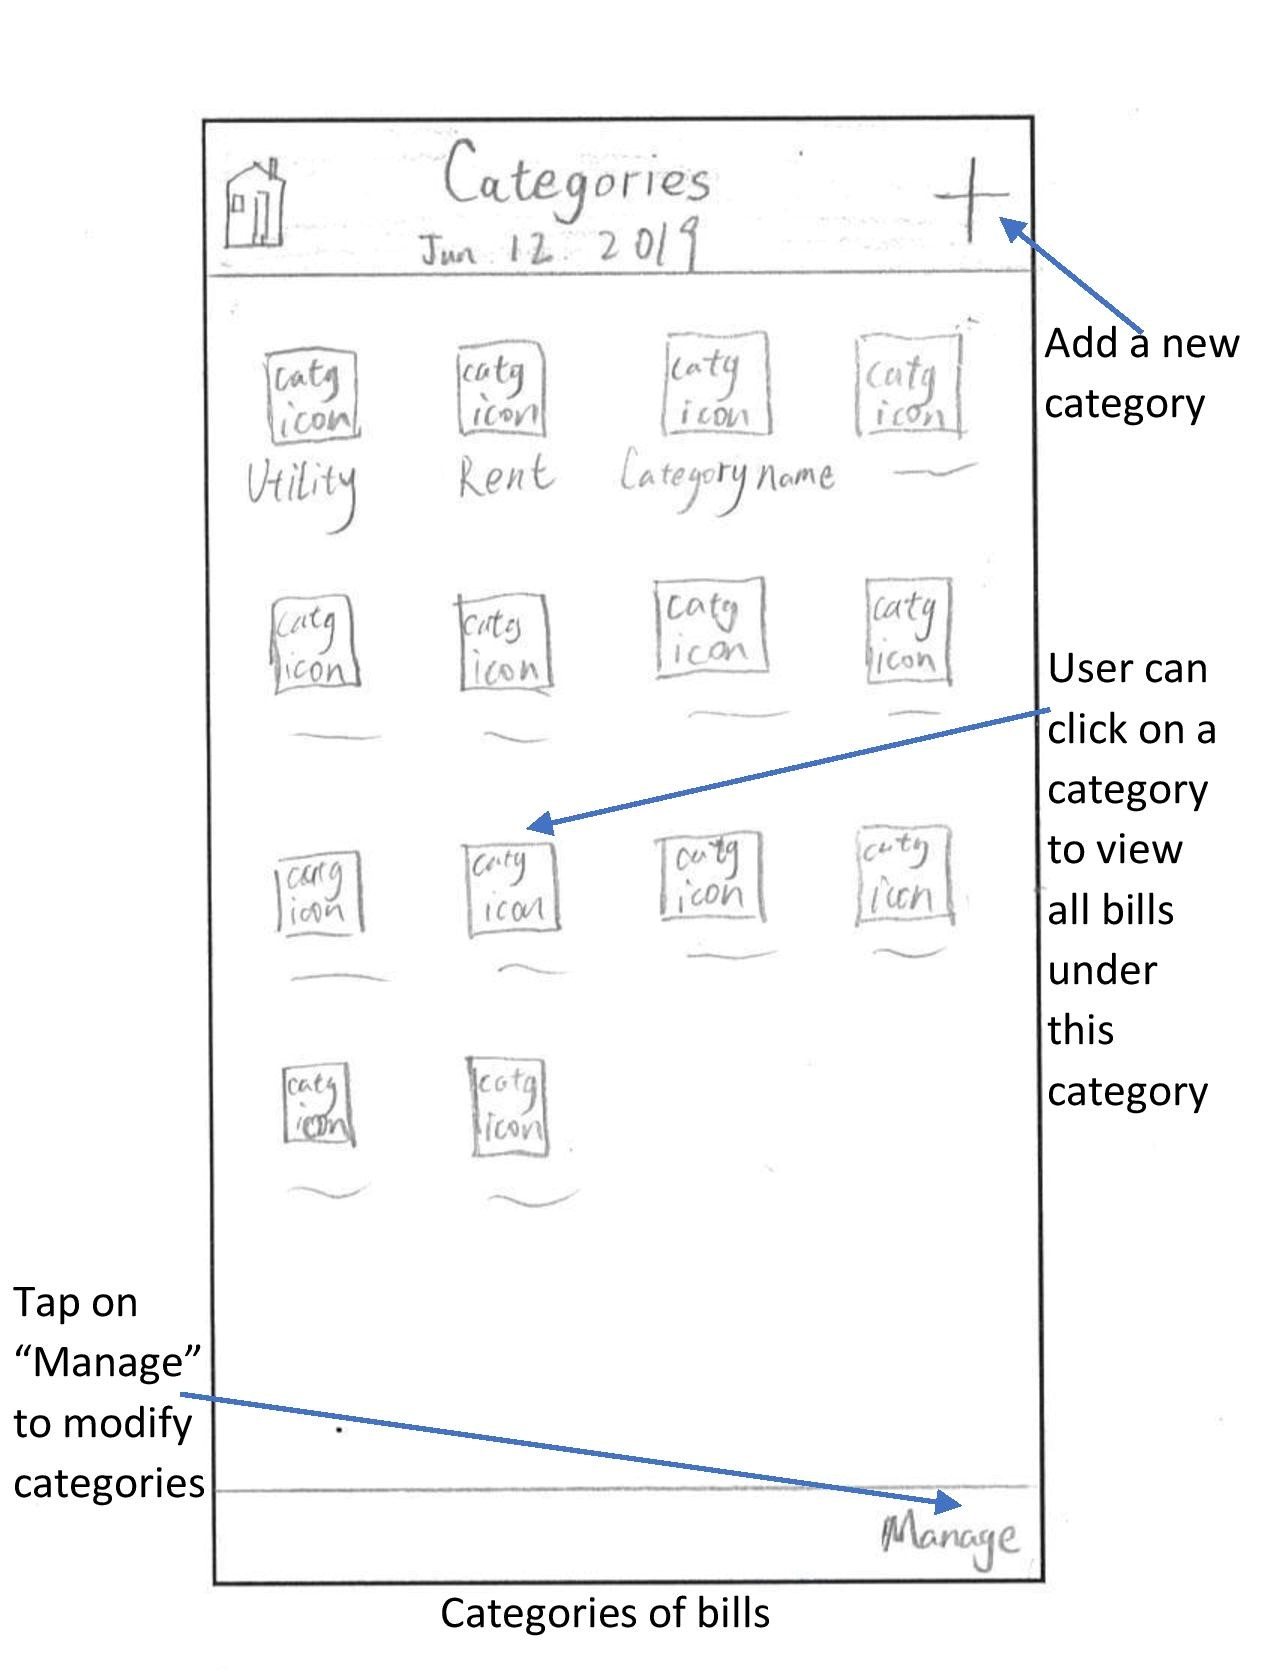
\includegraphics[width=0.6\columnwidth]{16-category-page.jpg}
  \caption{Sketch of categories page for application Billie}
  \label{fig:figure31}
\end{figure}
On the "Main/Home" page, the user can tap on the "Categories" icon to go to the "Categories" page as shown in Figure~\ref{fig:figure31}. Category icons are displayed in a grid view and each is associated with a category name. A user can click on a category icon to view all bills within that category. A user can also add a new category by tapping the "+" icon on the top right corner.  As a user, I want to customize the categories, so that I can better organize my bills. The "Manage" button on the bottom right corner will allow the user to manage existing categories.



\begin{figure}[h!]
\centering
  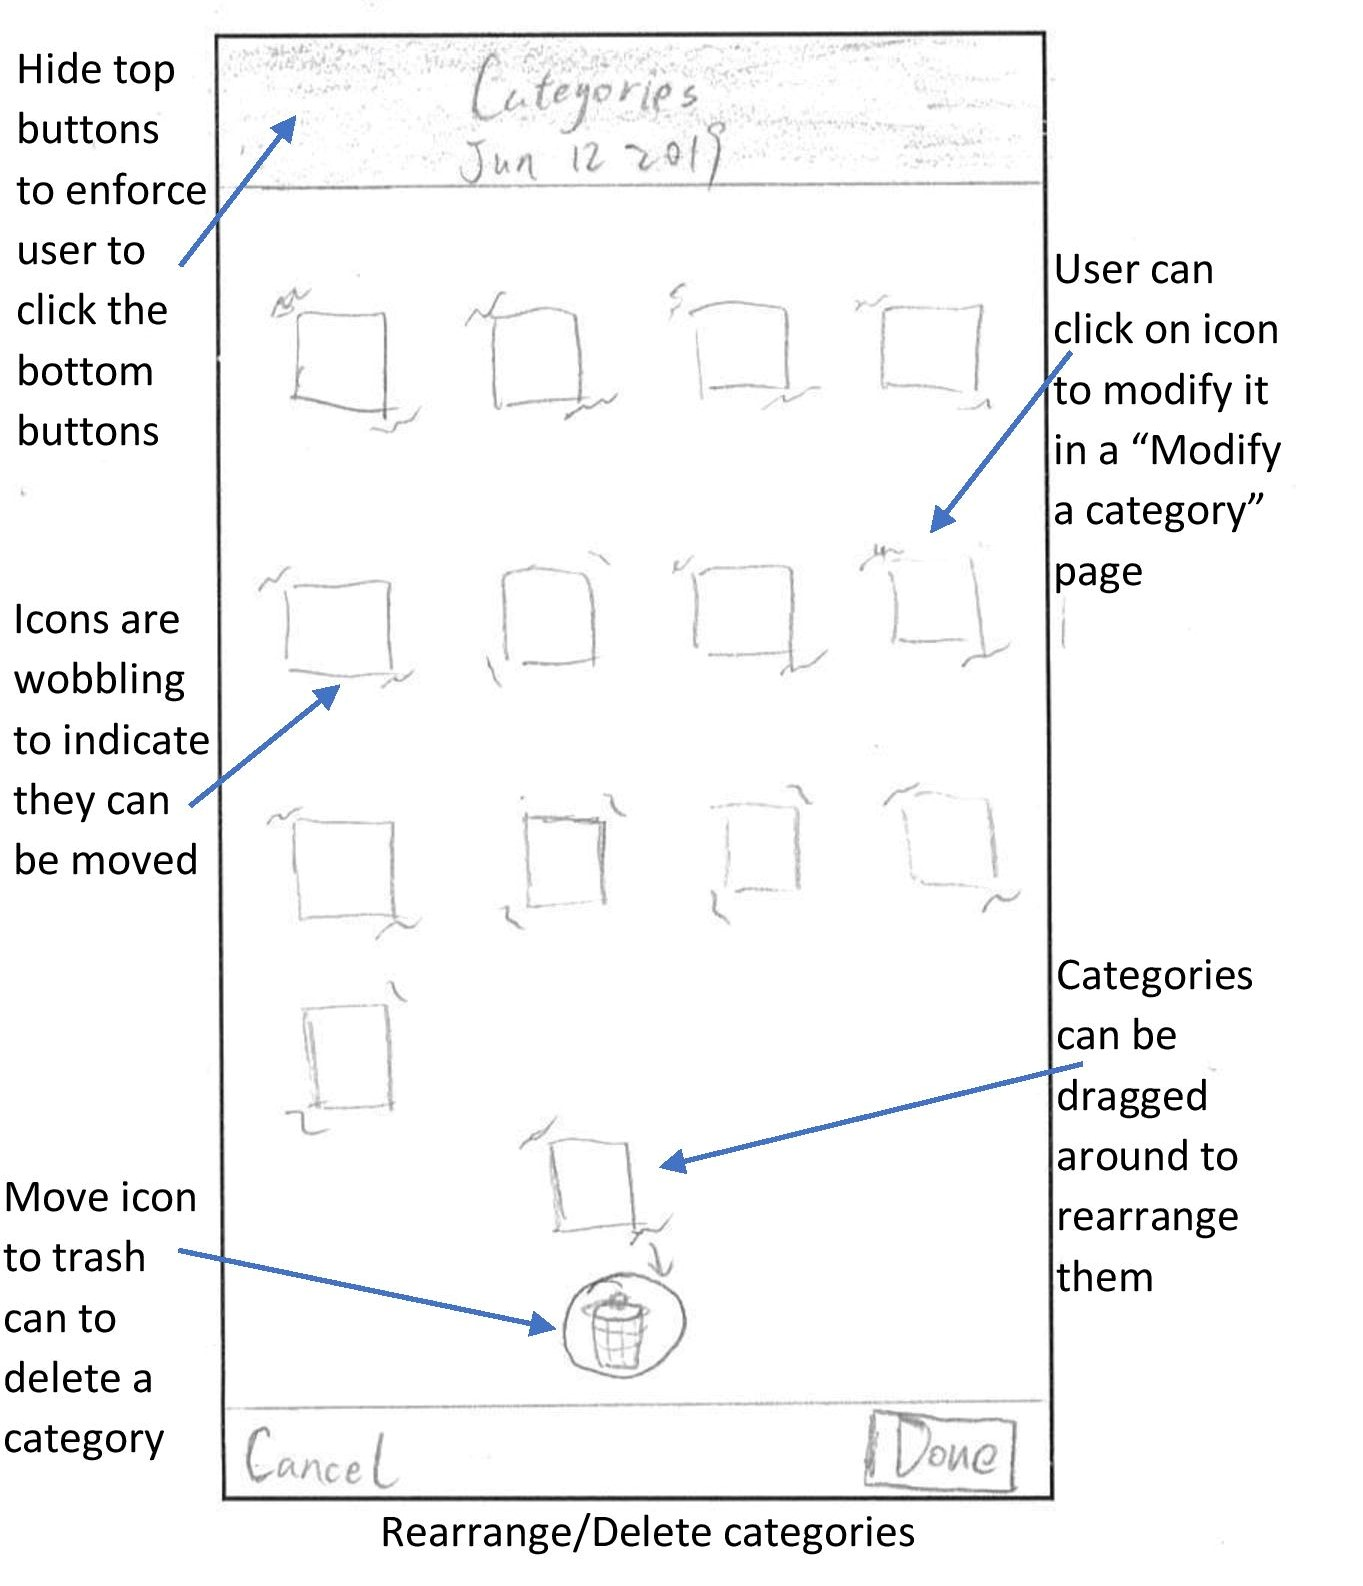
\includegraphics[width=0.6\columnwidth]{17-re-arrange-category-page.jpg}
  \caption{Sketch of managing categories page for application Billie}
  \label{fig:figure32}
\end{figure}
After tapping on the "Manage" icon, all the existing categories will start to wobble, indicating that they can be moved around for re-arrangement. As shown in Figure~\ref{fig:figure32}, a trash can icon appears on the bottom middle of the screen. Users can hold and drag a category icon to the trash can to delete a category. Tapping on a wobbling category icon can enter the edit page for a category similar to the "Add a Category" page. All top buttons are temporarily hidden to enforce the user to click the bottom "Cancel" or "Done" button to finish up managing.




\begin{figure}[h!]
\centering
  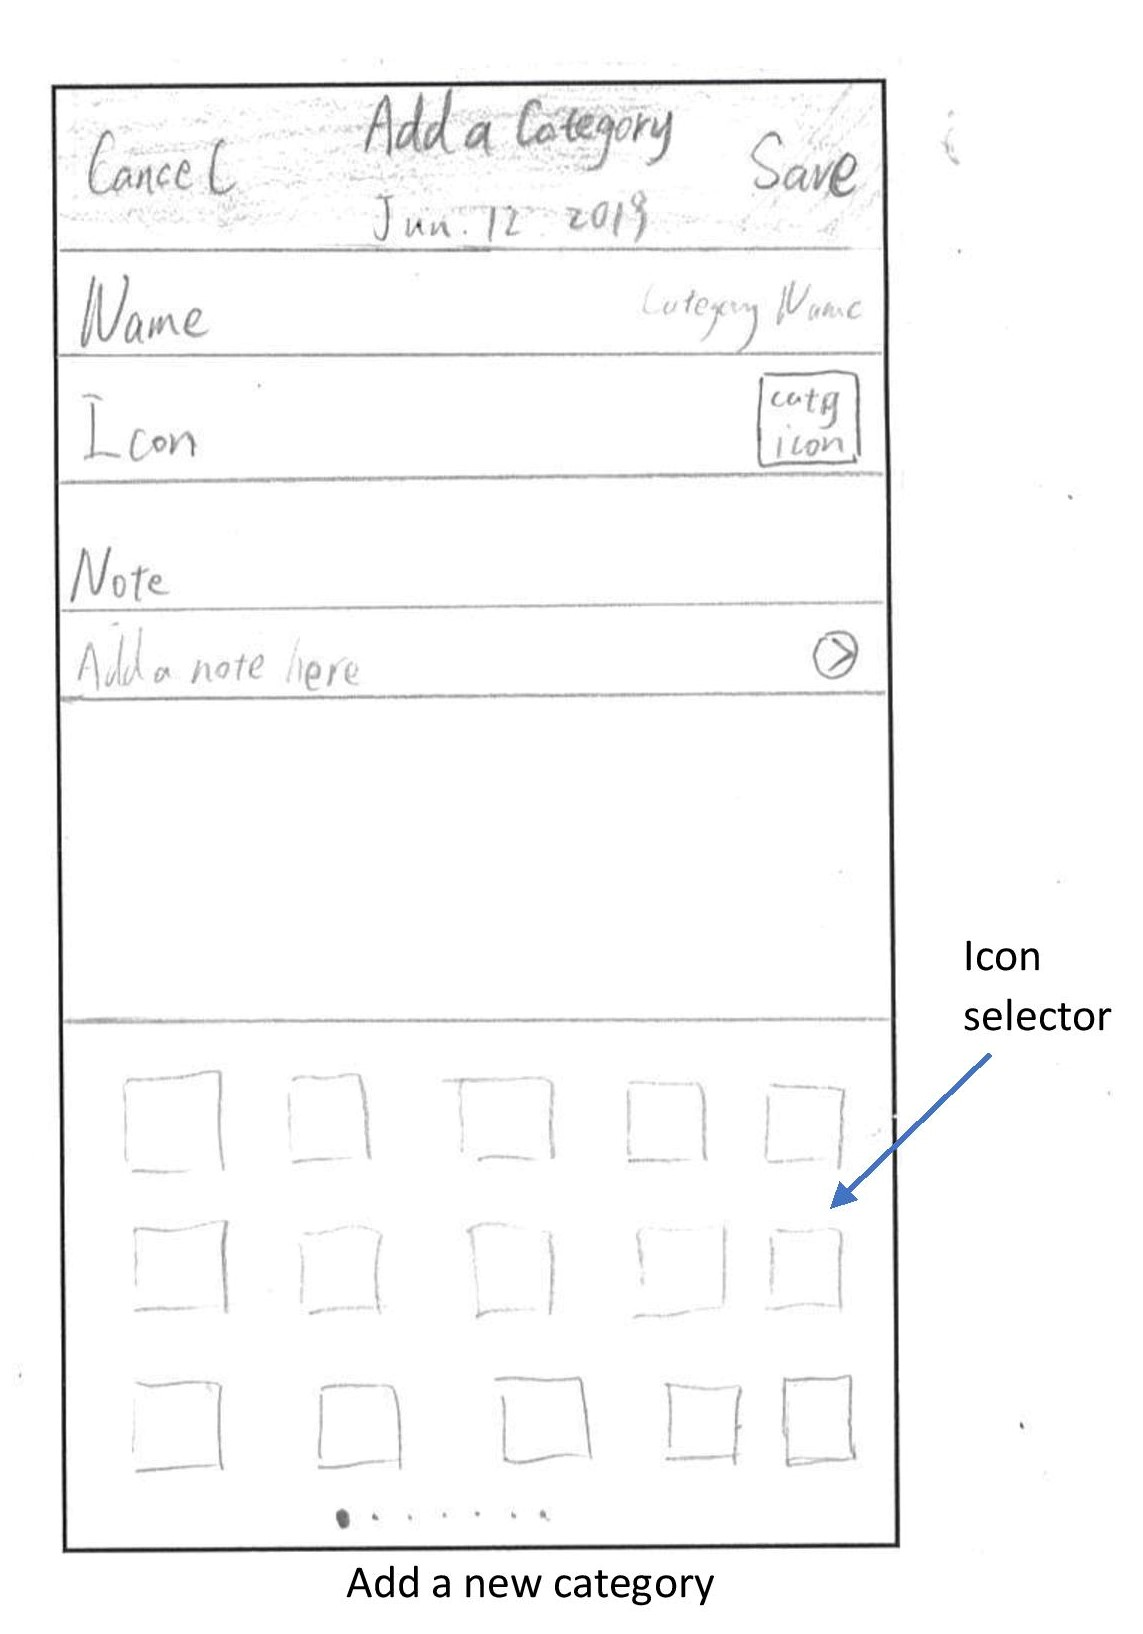
\includegraphics[width=0.6\columnwidth]{18-add-category-page.jpg}
  \caption{Sketch of add a category page for application Billie}
  \label{fig:figure33}
\end{figure}
As a user, I want to add a category when there is no category that fits my needs. In the "Add a Category" page, as shown in Figure~\ref{fig:figure33}, the user can enter the name of an icon and select the most accordant icon from the icon selector. The "Cancel" and "Save" buttons on the top can either discard or save the new category.




\begin{figure}[h!]
\centering
  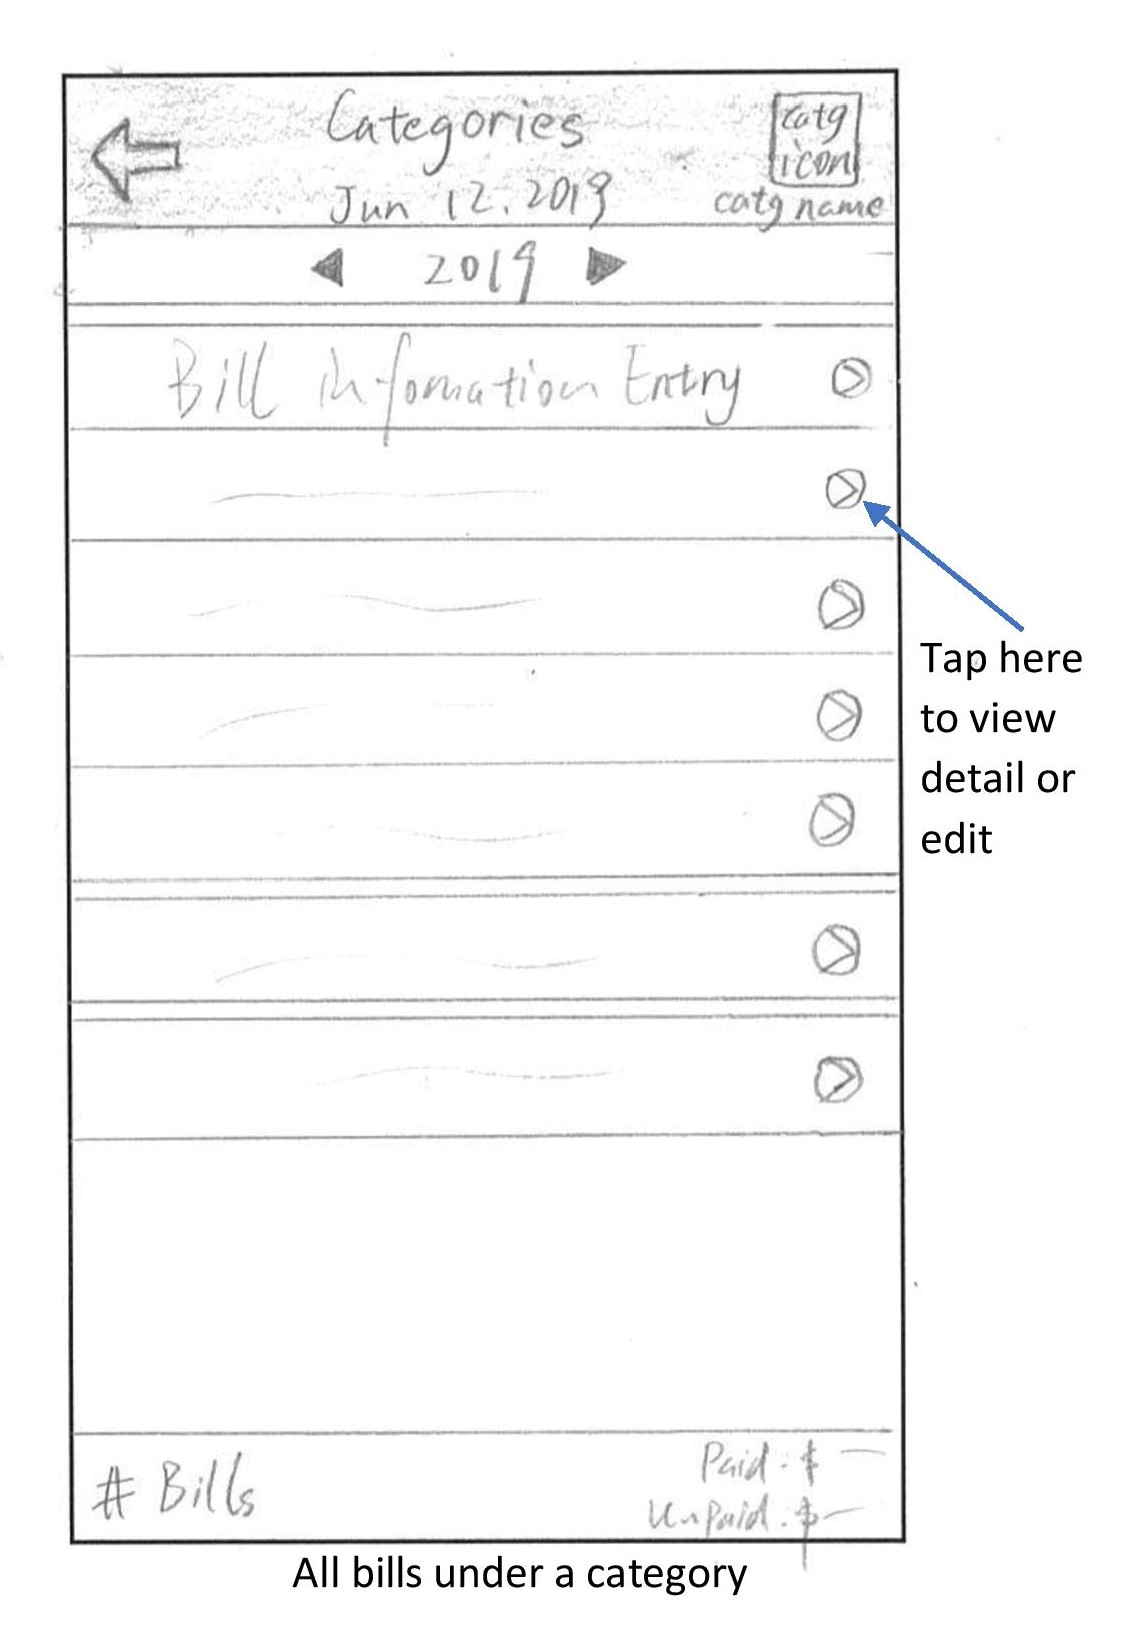
\includegraphics[width=0.6\columnwidth]{19-view-by-category-page.jpg}
  \caption{Sketch of view by category page for application Billie}
  \label{fig:figure34}
\end{figure}
As a user, I want to view all bills under a specific category. On the "Categories" page, the user can tap on any category icon to go to a category sub-page, as shown in Figure~\ref{fig:figure34}, to view the bills under that category in chronological order. An analysis bar similar to the one in the "list view" page is displayed on the bottom of the screen, showing the number of bills, paid and unpaid bills amount. Users can tap on any bill entry to view or edit the details.




\begin{figure}[h!]
\centering
  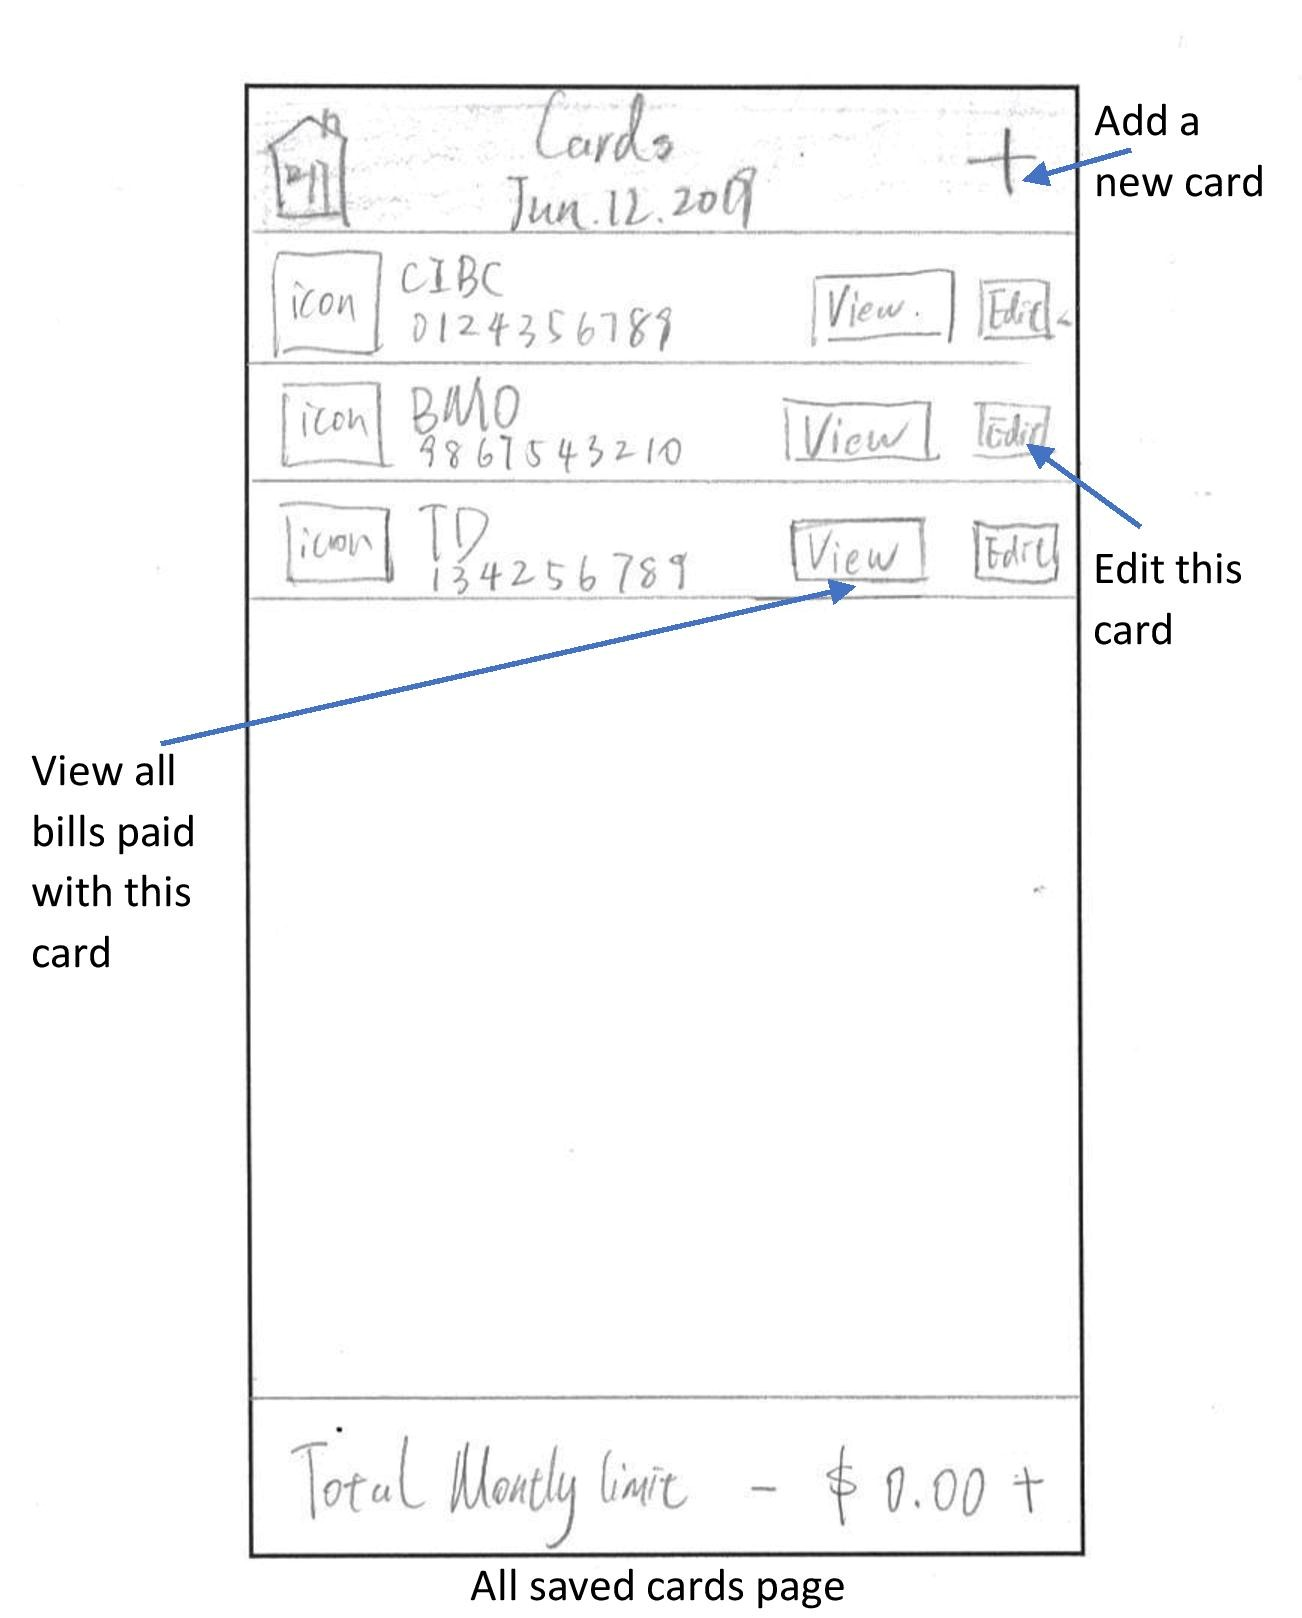
\includegraphics[width=0.6\columnwidth]{20-card-page.jpg}
  \caption{Sketch of cards page for application Billie}
  \label{fig:figure35}
\end{figure}
As a user, I need multiple-card support, so that I can easily manage bill payments from multiple cards with the same application. From the "Main/Home" page, the user can tap on the "Cards" icon to go to the "Cards" page, as shown in Figure~\ref{fig:figure35}. All saved cards are listed on this page. Users can either view all bills paid with a particular card or edit the information of a card. As a user, I want to set a monthly limit on my spending, so that I can do better in saving. The "Total Monthly Limit" on the bottom lets the user set a total monthly limit on all cards. When the total expenses approach the limit, Billie would send an alert to prompt the user to pay attention. The user can add a new card by tapping the "+" button on the top right corner.




\begin{figure}[h!]
\centering
  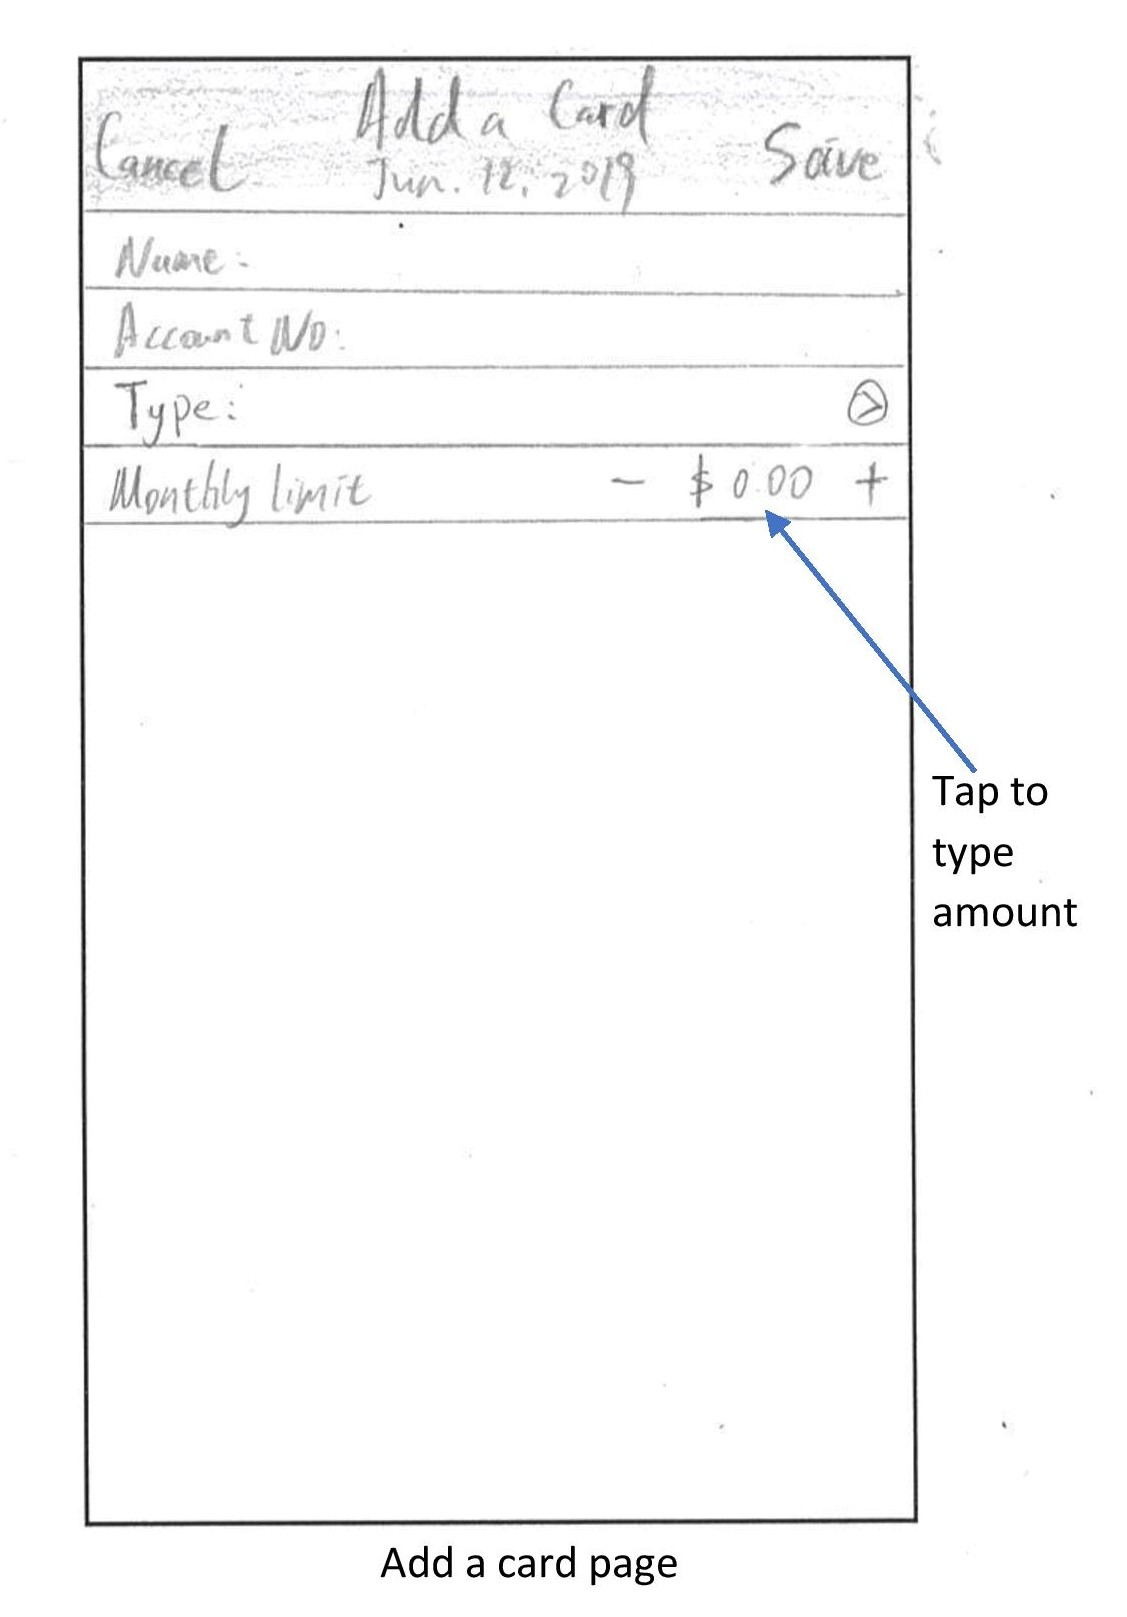
\includegraphics[width=0.6\columnwidth]{21-add-card-page.jpg}
  \caption{Sketch of add a card page for application Billie}
  \label{fig:figure36}
\end{figure}
As shown in Figure~\ref{fig:figure36}, the user can save a new card by entering its name, account number, and type. For security reasons, Billie does not ask the user to save the card's expiration date and 3-digit CVV number. The monthly limit feature is also available for an individual card.




\begin{figure}[h!]
\centering
  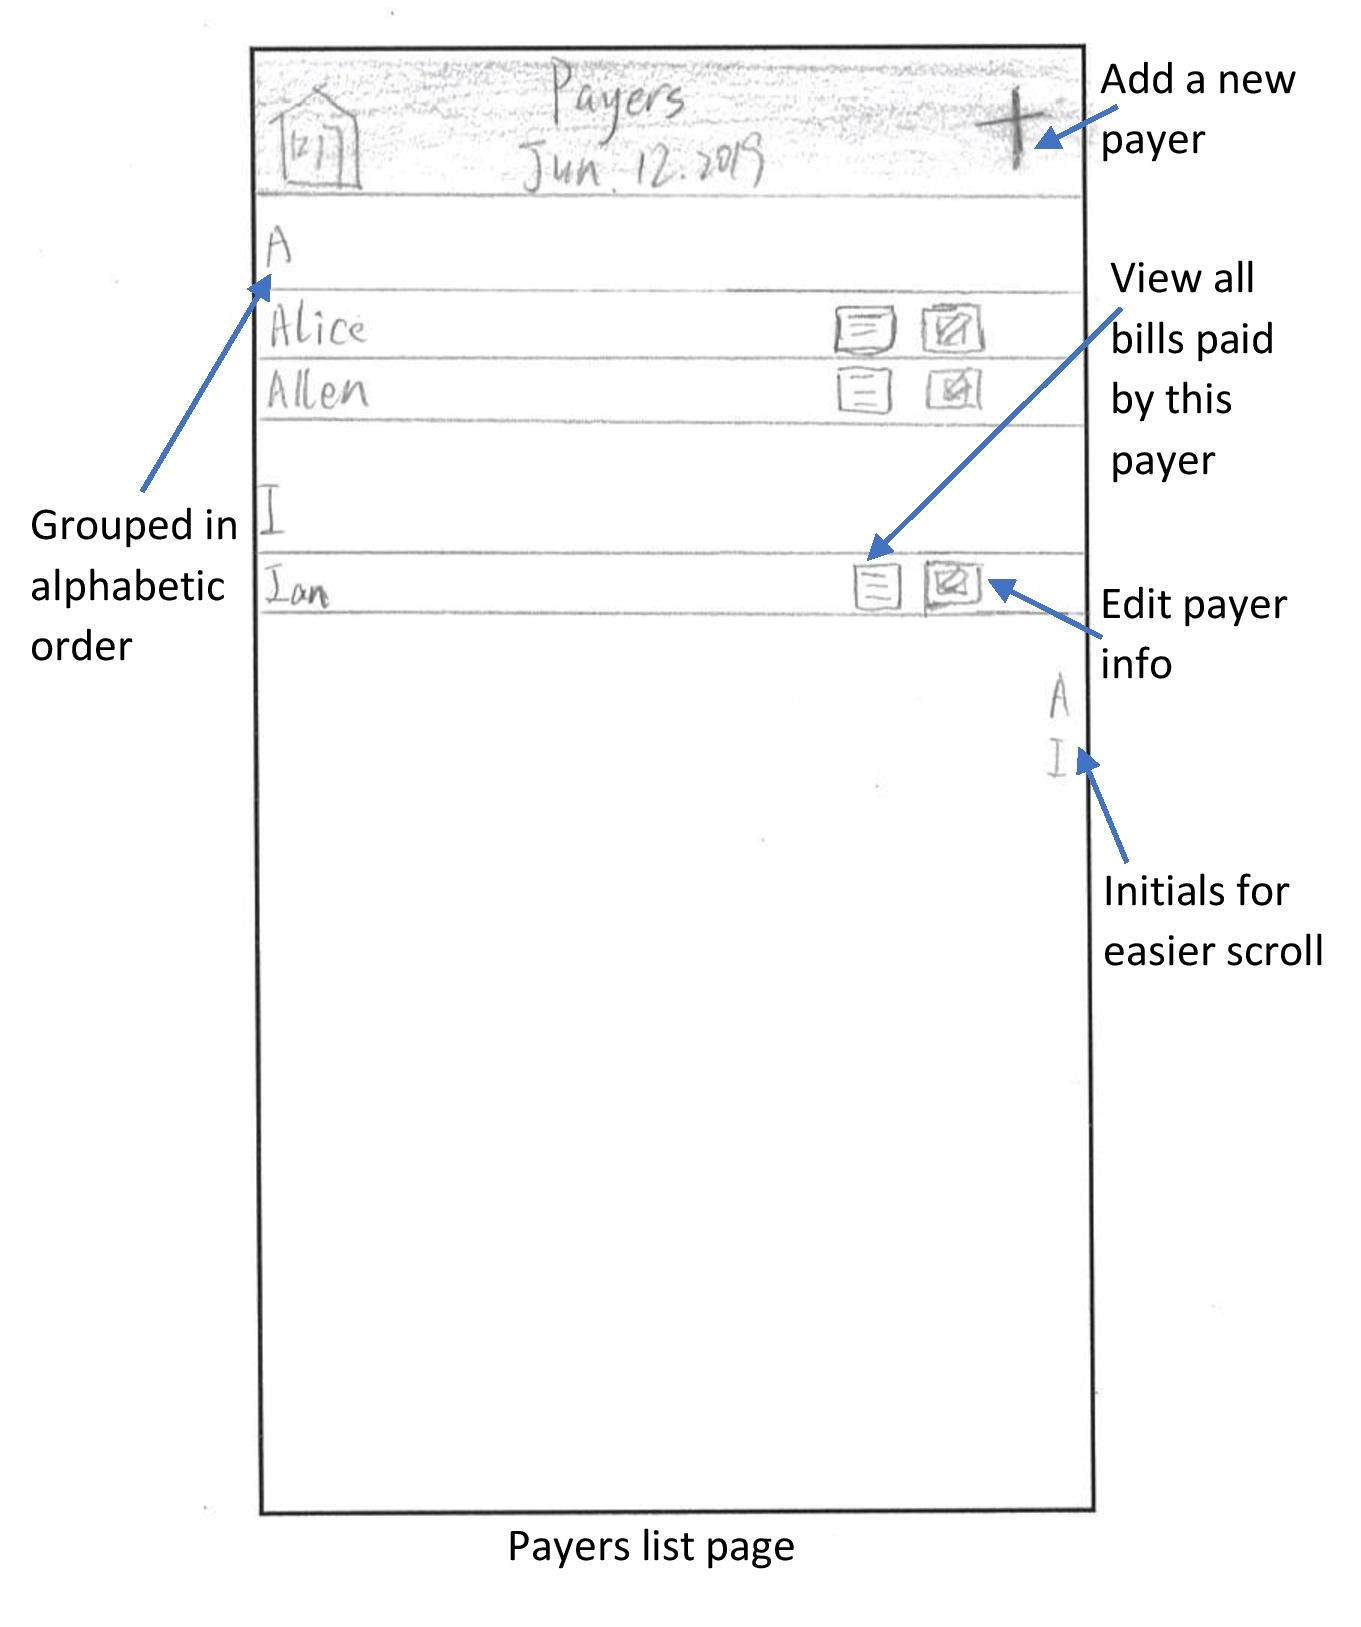
\includegraphics[width=0.6\columnwidth]{22-payers-page.jpg}
  \caption{Sketch of payers page for application Billie}
  \label{fig:figure37}
\end{figure}
As a user, I need a way to manage shared bills. On the "Main/Home" page, if a user taps on the "Payers" icon, he/she will be direct "Payers" page, as shown in Figure~\ref{fig:figure37}. The "Payers" page contains all the saved co-payers with the user. Payers are displayed in alphabetical order so that it is easy to find. Tapping on the left icon of a payer entry will show all the bills shared with this payer. Tapping on the right icon will allow the user to edit the payer info.




\begin{figure}[h!]
\centering
  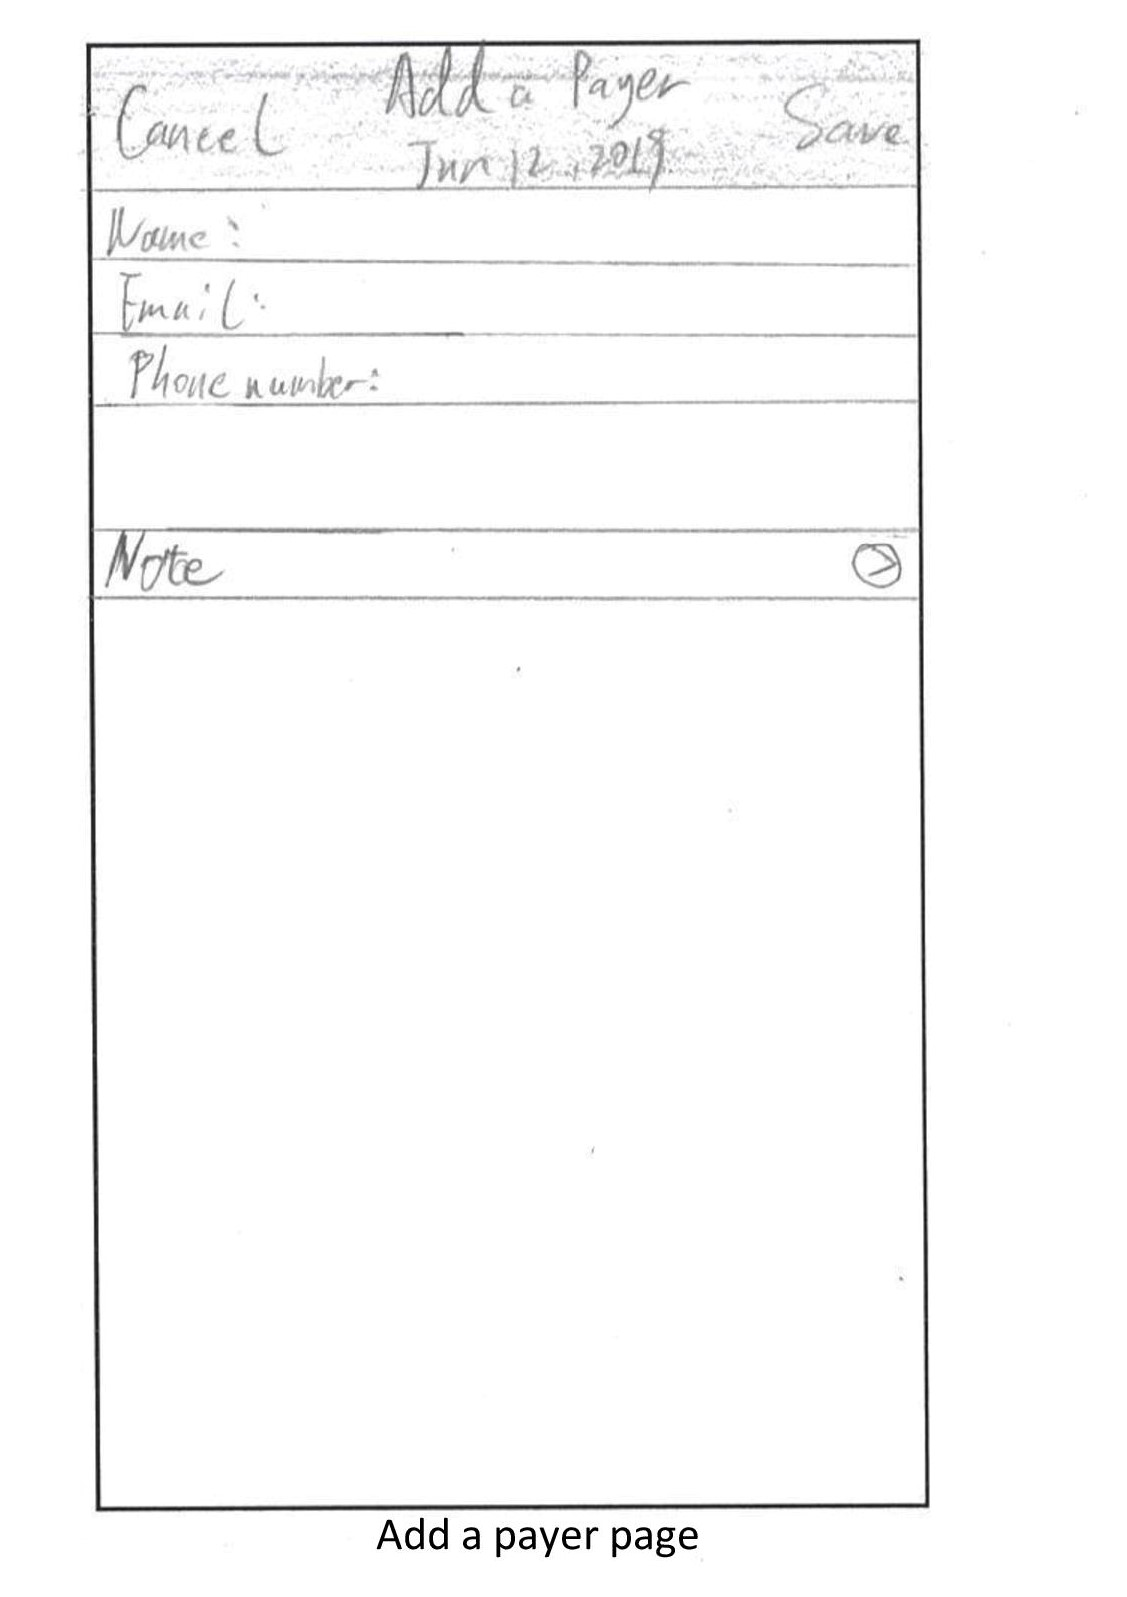
\includegraphics[width=0.6\columnwidth]{23-add-payer-page.jpg}
  \caption{Sketch of add a payer page for application Billie}
  \label{fig:figure38}
\end{figure}
By clicking the "+" icon in the "Payers" page, the user can "Add a Payer", as shown in Figure~\ref{fig:figure38}, into the payers' list. To add a payer, a user needs to know the co-payers' email or phone number or both. By clicking the "Save" button, the payer info is stored locally into the user's payer list. The co-payer would not receive any notification until the user bound this co-payer with a bill. 




\begin{figure}[h!]
\centering
  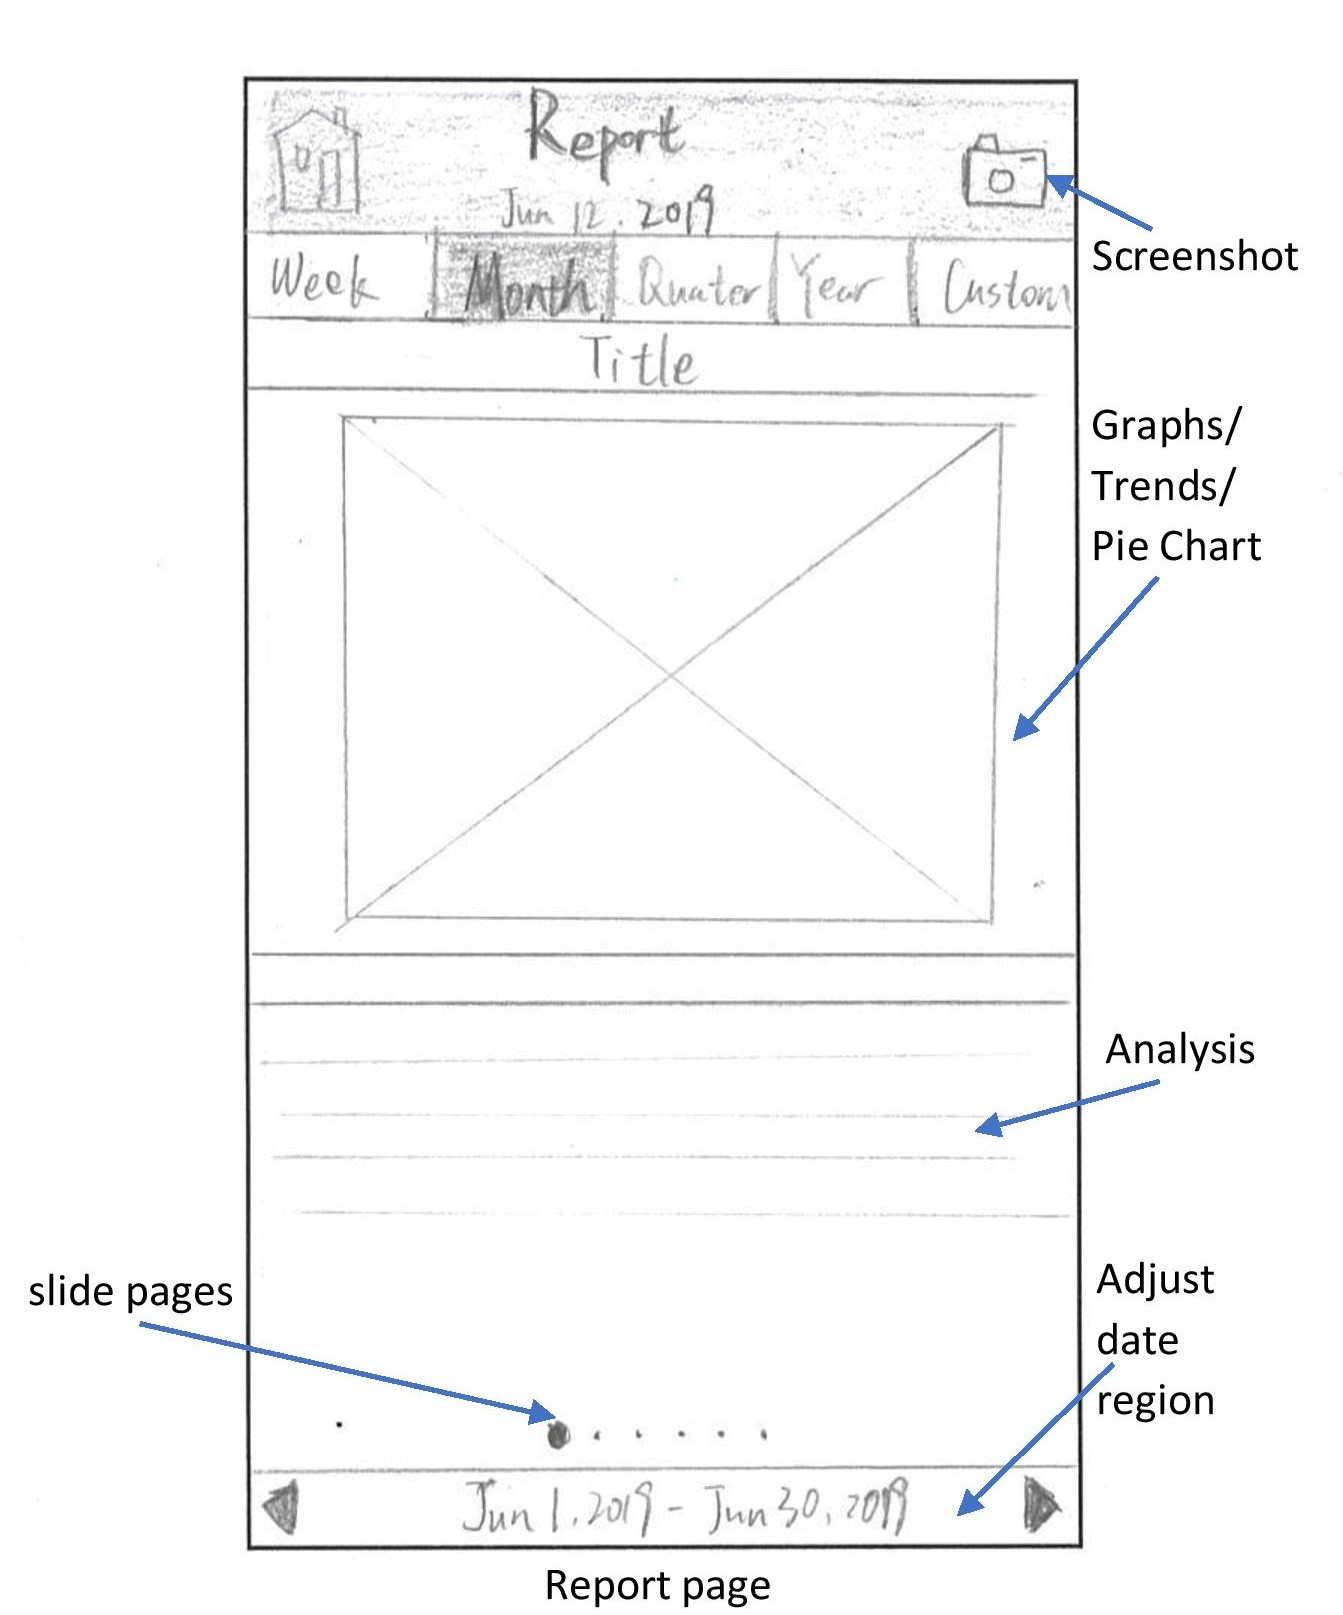
\includegraphics[width=0.6\columnwidth]{24-report-page.jpg}
  \caption{Sketch of reports page for application Billie}
  \label{fig:figure39}
\end{figure}
As a user, I want some reports with analysis, so that it can help me better understand my daily expenses, and ultimately achieve may saving goal. On the "Main/Home" page, the user can tap on the "Report" icon to go check on the reports. As illustrated in Figure~\ref{fig:figure39}, the time interval can be set in a week, month, quarter, year or any custom duration. The currently selected duration is shown on the bottom of the screen. Multiple kinds of reports are provided such as graphs, trends, pie charts, and analysis. Users can look through them by swiping left and right. A screenshot button is placed on the top right corner for quick access.

\section{6. Literature review}

In this section, some papers relevant to the challenges and design solutions are included. First of all, security is one of the major problems concerned by our participants. The paper by Dai Hong et al. ~\cite{RA} gives a brief introduction on mobile payment risk assessment and main characteristics. In the mobile payment protocol, there are usually four roles involved, which are User, Business, Financial organ, and Payment gateway. Besides, the flow of complete mobile payment includes ten steps starting with registration and ending with feedback to consumer. During this process, the system needs to deal with not only the traditional information security risks but also risks with multiple threat sources, multiple threat behaviours, and various adverse consequences. Therefore, we need to divide the whole mobile payment system into five sub-systems and analyze the risk assessment targets. In addition, Christen Hahn et al. ~\cite{MP} talks about the major challenges in mobile payment security. Basically, the transactions on a mobile device can be conducted via Short Message Service (SMS) messages, at a point of sale (POS), and online in the Internet. The mobile payment has gained its popularity in many regions. During Chinese New Year in 2015, millions of new linked their bank accounts to WeChat for signing up WeChat's red envelope program. After that, the mobile payment systems can be divided into five categories, which are mobile payment at the POS, mobile payment as the POS, mobile payment platform, independent mobile payment system, and direct carrier billing. Next, mobile payment security is explained and the main mechanisms are Fingerprint, Username/password, Multi-factor authentication, SSL/TLS, and Secure Element. Finally, mobile payment also faces many serious challenges, such as malware detection, multi- factor authentication, data breach prevention, and fraud detection and protection. Therefore, according to the previous articles, security is a challenging issue in mobile payment and we include several mechanisms such as Fingerprint and User name/password to improve the security level of our application.
 
Besides, payment behaviour is also related to our design solution, and Scott Schuh and Joanna Stavins ~\cite{Pay} have found that the characteristics of payments are important in determining consumer payment behavior. They firstly collect data on nine different payment instruments including cash, check, money orders, credit cards, debit cards, and so on. By analyzing the data, it is observed that the overall rate of credit card adoption is 78 percent, and the rate of debit card adoption is 80 percent. In addition, cash and debit card use is higher for younger, lower income, less educated respondents; credit card use is higher for older, higher income, more educated consumers. As for payment characteristics, the authors have built a mathematical model and found that credit card adoption is affected by record keeping, ease of use, and control over payment timing. Also, setup and record keeping are important in debit card adoption. Other than that, setup and security are the most significant ones in BNA (Bank Account Number payments) regression and OBBP (Online Banking Bill Payment) adoption. Hence, debit and credit cards play important roles in the payment process, and our application is designed mainly for this payment instrument.
 
Moreover, saving goals are mentioned a lot by our participants and it would be helpful to study their saving motives. Luigina Canova et al. ~\cite{Saving} represent the saving goals in a hierarchical structure and perform network analysis on the goals. In the paper, the data are collected by questionnaires on financial and saving questions, then the authors group a total of 943 super-ordinate goals and separate them into different categories. Based on their results, self-esteem and self-gratification are the highest-order goals from psychological perspective. Besides, people want to avoid debt and achieve a certain security level in their life. In addition, purchases and money availability are significant reasons for saving. However, age/illness are also major motivations for people who want to maintain a good standard of living after retirement. Therefore, saving goals are necessary not only for middle-aged and senior people but also for young people. Students are our target user group and they need to set their own saving goals, so we add the functionality in the application.


Finally, bill sharing problem is the focus of the application, and it would be helpful to learn Azadeh Forghani et al. ~\cite{Forghani} bring up the idea of G2G, which is a shared calendar and video messaging system to connect young children with their grandparents over distance. As for the shared calander, children and grandparents can add their daily events, activities, thoughts or feelings through stickers categorized in several main categories. Also, any added stickers are shown on both the grandparent and grandchild's version of the calendar; the views are reciprocal. By integrating messages with shared calendar, it provides a technology that supports mutual awareness about daily life and therefore can help grandparents and grandchildren to get to know each other better feel more emotionally close. Besides, both parties can add event to the calendar by simply selecting a day from the calendar. Therefore, shared calendar is a smart way to share visual information and communicate efficiently. 



\section{7. Paper prototypes and evaluation}

\subsection{7.1 Description of goals and hypotheses}


First, we want to test the privacy and security features, including features such as account sign up, sign in, sign out, set up a PIN and biometric authentication. We want to find how users like the setup process. Do they find the procedures intuitive and easy to follow? Or do they find them complicated and redundant? Does this level of security powerful enough for the users to trust saving their valuable bill information in our application. Or is there any extra security and privacy features that can improve users' confidence? We assume that users will prefer to use the on-device biometric methods to sign in instead of using a password or PIN since nowadays most of the smartphones have those features and people are used to them because of their simplicity and a higher level of security. The re-entry authentication feature is also expected to be a success since it adds more security to the application especially under the circumstances when someone peeks at or stole an unlocked phone.

Next, we want to test the procedure of adding a bill to Billie, since it could be the most frequently used feature. We want to see how long does it take for them to add a bill manually. Do they find all the attributes helpful? Or do they leave some of them blank? We can make put the high priority attributes above the low priority ones, and separate them by required and optional. Do they find the Auto-Fill feature speeding up their bills recording process? Do they find the repeat and remind attributes has good options? How do they normally split bills? What if they want to add a payer in a shared bill when this payer is not in the payers' list? Can they still do it? We expect the Auto-Fill feature to be successful since it not only speeds up the filling process but also keeps an image of the receipt of the bill, which may come in handy in the future. Shared bills feature is also highly anticipated to be a success because it simultaneously benefits multiple users.
 
Next, we want to test the different ways to view saved bills. We have a list view, a calendar view, view by category, view by payers, view by cards, view by search. We want to see which way does the user normally use to view their saved bills. Do they find each way of view the bills well organized? Or do they feel it was a mess? Can they easily view and edit the details of a bill? Can they pay within Billie? Do the saved account, password, and card number help them along the payment process? We expect the calendar view to be successful since it is normally how people mark down the important matters in our lives. The built-in web browser is also expected to be a welcome feature because it saves the effort of needing to open an external browser to pay bills. It centralizes the bill management and payment procedures all within our application.

Next, we want to test all the supporting features for adding a bill, such as card management, category management, and payers contact list. These features are used less frequently, since they can be set up once, and later only make changes or additions when needed. We want to see if the correlation with a bill is intact and robust. Do the users found these features has a well-balanced level of customization? Or do they feel they want more or less? How do they find the process of adding a card, category or payer? How about edit the existing ones? Does setting the monthly limit help saving? We assume that all the customization will be appreciated since users can adjust configurations to better fit their needs and making their bill management more efficient.

Finally, we want to test the report feature. We want to see if the users find the different kinds of reports helpful for achieving their savings goal in the long term. 


\subsection{7.2 Description of the participants}

According to our user group, we have selected 4 participants with average age 24-year-old from Waterloo-Kitchener Area, Canada. In addition, all the participants have shared bills with others and at least one roommate by the characteristic of our target user group. Also, in order to get some diverse results, our participants are of different genders (3 male, 1 female), education levels (2 undergraduate, 2 graduate), family status (3 single, 1 married).

\subsection{7.3 Set of goal based tasks}
The goal based tasks for the paper prototypes evaluation are stated as follows:

\begin{enumerate}
\item Please open up the Billie application.
\item You are on the welcome page now. 
    \begin{enumerate}
        \item You don't have an account yet. Now you want to sign up for an account. How would you do that?
        \item You already have an account. Now sign in to your account. How would you do that?
    \end{enumerate}
\item Now you are on the main/home page. You want to ensure that your account as protected as possible. How would you do that?
\item You want to change the default currency to CAD. How would you do that?
\item You want to get back to the main/home page. How would you do that?
\item You switched to another application and now bring Billie back from the background.
    \begin{enumerate}
    \item Suppose biometric authentication is on and working. You want to enter Billie. How would you do that?
    \item Suppose biometric authentication is on but failed to work. You want to enter Billie. How would you do that?
    \end{enumerate}
\item You just ate at a restaurant and got a receipt of a total value of \$15.33 paid with your previously saved CIBC debit card. You want to save a record of this bill by adding this bill to Billie. How would you do that?
\item You had 3 friends came over last night and there is a total expense of \$87.58 paid with your new BMO credit card that you want to share evenly within your group of 4. How would you do that?
\item You want to view your expenses within the last week. How would you do that?
\item You want to view the upcoming bill dates. How would you do that?
\item You locked your screen. Now you received a notification saying that you have an electricity bill of amount \$35.13 is about to due in 3 days. But you decide to pay it now within Billie. How would you do that?
\item You want to view your bill report from May 1 - May 31, 2019. How would you do that?
\item You found you spend too much recently. And you want to set a monthly limit on your card. How would you do that?
\item Now you want to sign out of the account. How do you do that?
\end{enumerate}


\subsection{7.4 Paper prototype evaluation results}

Most of the goals are met through the evaluation. Firstly, we have tested the registration process and the authentication information set up procedure. The participants find the registration process easy to follow and they are able to complete independently. Also, based on their prior experience, they can set up and apply the biometric authentication without any difficulty. After that, we have asked participants to fill in the attributes for adding a new individual bill and a new shared bill. Other than that, we have partially tested different ways to view bills. When asked to view the bills in the last week, the users tend to use the "Report" feature instead of scrolling down in the "List view". With viewing upcoming bills, people prefer "Calendar view" to "List view". In addition, as for testing other supporting features, such as "Select a card/a category/payers" or "Add a payer", the goal is met. Because the participants need to try out the functionalities when they are asked to perform an add-a-new-bills task. The task for setting up a threshold limit for cards is also easily performed. Finally, the goal for testing report feature is met. However, some of the goals are not fully met and we think the reason is that there are too many features included in the application and it is hard to evaluate all of them within 15 minutes of paper prototype testing. Besides, the naive participants do not have enough time to walk through the whole application so that they are not aware of some hidden functionalities. For example, the "Auto-Fill" feature is ignored in the first place or half-way through the "Add bill" process, but they would like to use it if they had noticed it. In summary, the study design reflects the goals well. Each task gives the participant a real-life situation in the bill management process, and each element is tested separately. Besides, we are able to test the paper prototype from various aspects and the participants need to complete the required tasks based on their own experience as well as different cases.

Furthermore, the discovered themes and detailed results of the paper prototype evaluation study will be discussed. To begin with, all participants found that the application contains too many functionalities and they may not use all of them. We think the reason for that is there are some unnecessary features included in the design and make the application too complicated to use. The "9-grid" home page layout makes those small features look evenly important as the main ones. We should focus more on the depth instead of breadth so that the application can solve one particular problem better. Besides, users prefer to use fingerprint than passwords when they re-enter the application, which corresponds to our hypothesis which says "biometric authentication is a good design that increases the security level". In addition, the participants are able to add a bill and fill in the attributes with the supporting features such as card management, category management, and payer list. However, users take more time than we expected to complete adding the new bill. Participants feel that some of the fields are redundant. We think the reason for that is there is no distinction between mandatory and optional attributes so the user will to complete all fields. Besides, as for shared bills, some participants are not aware that all the co-payers will be notified when a new shared bill is created. We think the reason for this problem is that the functions available for the shared bill feature are not clear enough. Also, people tend to use calendar view more than list view when they are asked to look at upcoming bills, which means the calendar view feature is a good design and our hypothesis is verified. Other than that, the auto-fill functionality is not noticed by participants in the first place. We think the reason for that is they have not prior knowledge and the position of the auto-fill button is at the bottom right of the page. When the users are aware of the auto-fill button, they prefer using it than typing manually, so it is considered a good design and the hypothesis is verified. Nevertheless, some users do not notice that they are able to pay bills within the application using the built-in web browser. All participants do not want to save their payment account inside the application and prefer not to pay within the built-in browser, either. Hence, the result does not correspond to the hypothesis, which assumes the built-in browser to be a good design. We think the reason for this is people are concerned about privacy and security. Finally, all participants find the report helpful because they can view all the expenses by different categories and achieve saving goals more efficiently. 

The descriptive images for paper prototypes are attached in Appendix. 

\section{8. Design progress}

Based on the result of the paper prototype testing, in order to get the right design, we made a nearly complete overhaul to the initial design. The key differences for this second generation design compared to the original design are 1. Make the key features stand out from the supporting features; 2. Reinforce the shared bill features; 3. Getting rid of unnecessary features; 4. Unity across the application

First of all, as shown in the "Appendix-Wireframes with Descriptive User Flow" (AW)-Figure~\ref{fig:figure40}, the welcome page, the sign in and sign up features and processes remain unchanged, since none of our participants were having issues during these steps. The sign in and sign up methods and processes follow the current standard on most other mobile applications so that the users are very familiar with them and can get around them fairly easy with no complaints. As for now, users can sign up with either their email or mobile number.

After signing in, the users will see a completely new design of the main page, as shown in AW-Figure~\ref{fig:figure41}. The users will see that at the bottom of the screen, Billie is now split into 3 tabs: "View Bills", "Groups", and "My", corresponding features respectively to viewing history and upcoming bills, managing shared bills within a group, and managing other supporting features. Comparing to the initial design of the Main/Home page shown in "Appendix-Descriptive images for paper prototypes" (AD)-Figure~\ref{fig:ADfigure9}, which has a 9-grid square item layout that treats all features equally, this new iteration of design will bring the users straight into the List/Calendar view of bills under the "View Bills" tab. We made this change because we identified that "View Bills" is one of the top priority features which the users would be eager to use as soon as they open Billie. Therefore, instead of letting the user have an extra selection, Billie now presents the users with a list starting with their most recent upcoming bill at the very top, so that the users can easily take a glance and have the important things in mind. Based on the paper prototype study, we also identified that some users also prefer the calendar view of bills. So we provide the users with a way to easily switch between the list and calendar view by tapping one time on the "View Bills" tab. A corresponding icon on the "View Bills" tab will enlarge, indicating Billie is now in that view.

In the list view shown in AW-Figure~\ref{fig:figure41}, bills are listed in chronological order and grouped by months. Each bill is a concise entry with the most important information displayed. A scroll bar is presented on the right side of the screen when information is not fully presented on one page so that users can scroll up and down to view history or upcoming bills within a calendar year shown on top. Users can tap on the left and the right arrow beside the year to change to previous or next year. When more and more of the bills are saved, it may cause a problem to find particular bills. Therefore, we kept the search feature in the previous design, but put it right on top of the list of bills as a small user-friendly feature for users to search by name, card, payers, etc. to find particular bills. All paid bills are faded out for clarity. Users can tap on a bill entry to view or edit the detail of this particular bill. In the calendar view also shown in AW-Figure~\ref{fig:figure41}, a calendar month is presented. There will be a red dot beside every date with at least one unpaid bill. All past paid bill dates will be indicated by having a check mark beside the date. Users can tap on the calendar to choose bill dates and all bills due in that day will be listed as bill entries below. In both list and calendar views, when users navigate too far away from the current date, user can double tap the current date under our application name "Billie" to quickly locate back to the most recent upcoming bill. We feel like the changes we did with the home page and with the way we provide users to view their bills significantly make the "View Bills" feature stands out and make the important information better presented.

On the top corners of the "View Bills" tab, the users will find two more buttons, "Bill Alerts" and "Add Bill". In fact, these two features are presented on the top corners of all three tabs. We put these two features up there for easier access because they are also the top features we identified. "Add Bill" feature perhaps is the most used feature of Billie, since users need to keep adding new bills into the application to actually make Billie useful. By clicking on the "Add Bill" icon, users will be prompted with an "Add a Bill" screen shown in AW-Figure~\ref{fig:figure42}, where users can record either a personal or a shared bill by choice. There are several fields to a bill that is listed to be filled on the page. From the paper prototype testing, we learned that the users feel that all fields are required to be filled while some are optional. Comparing to the initial design shown in AD-Figure~\ref{fig:ADfigure11}, now we get rid of some of the unnecessary fields such as websites, username and password because we are getting rid of the feature to pay bills within Billie using a built-in browser shown in AD-Figure~\ref{fig:ADfigure24}. We also marked all required fields with "*" at the front. The Auto-Fill feature is now more emphasized, taking up the whole bottom space as shown in AW-Figure~\ref{fig:figure42} while we are getting rid of the calculator feature shown in AD-Figure~\ref{fig:ADfigure24}. Comparing to the initial version, now the Auto-Fill feature is more visible and the fields are more concise. So whenever the users have the receipt, they can easily use the Auto-Fill feature to scan it, save a digital copy of it, and save the hassle of manually typing in those fields. Some of the fields are hidden for non-recurring bills for simplicity since we identified that recurring bills are recorded less frequently than the non-recurring ones. Those fields only show up when the "Recurring" toggle is turned on as shown in AW-Figure~\ref{fig:figure42}. Some fields with selection entries such as card and category will prompt the user with a dedicated "Selection" page. For shared bills as shown in AW-Figure~\ref{fig:figure43}, more fields are required. A payers selection page will allow the primary payer to add co-payers within a shared bill so that all payers are synced with this particular bill in their account as well. Comparing to the initial design for the "Add Bill" feature, this version gets rid of or hidden many unnecessary features, providing users with a clearer view.

From the paper prototype testing, we know that we need to make the shared bill feature more robust and visible. Therefore, we emphasized this functionality substantially by adding a completely new "Group" tab as shown in AW-Figure~\ref{fig:figure44}, for better co-payers' communication. Whenever a shared bill is created, all the co-payers related to this bill will receive a request to be added. And by confirming, they will all be formed into a group dedicated to this particular shared bill among them. By tapping on the "Groups" tab, the users will see all the "On-going" shared bill groups they are currently involved in and all the history shared bill groups in "Archive". The red numbered badge reminds users of the unread messages from groups. Each group entry corresponds to a shared bill with the same name. The users can see their identity within this shared bill, as either the primary payer or a co-payer. A search bar is also provided to search for particular groups when shared bills pile up. An on-going bill cannot be deleted, while an archived bill can be deleted by making a left swipe. Co-payers will continuously receive notifications from a shared bill group until their debts were cleared and confirmed by the primary payer, then the group will mute. The primary payer will continuously receive notifications from a shared bill group until all debts are received and confirmed. The shared bill ends and the group moves from on-going to archive only when all debts are cleared by the co-payers and confirmed by the primary payer. Based on this double-checked principle, the functionalities within a group for a primary payer and a co-payer differ from each other. In the primary view's view as shown in the middle screen of AW-Figure~\ref{fig:figure44}, he/she provides details and reminders for the co-payers to remind them to clear their debts. When a co-payer indicates already paid, the primary payer has the option to perform a confirming action by long press the message from the co-payer. If checked, the co-payer will be released from the reminders and the system would send an updated for all other unpaid co-payers. For the co-payers, we identified that the reasons for not paying back is often just forgetting, instead of not willing to pay. So they would actually want to be reminded until they pay back. So they can perform only two options in the group as shown in the right screen of AW-Figure~\ref{fig:figure44}, one telling the primary user that the bill information is noted, the other telling the primary user that the debt is cleared. Since this is a completely new feature added to this version, we still need to perform some tests on it. But compared to the shared bill features in the initial version, this will definitely improve the communication among co-payers. 

When users are not using Billie, it will still remember all the saved bill information for users and remind them with notifications as shown in AD-Figure~\ref{fig:ADfigure21}. By tapping on the notification, the user would be brought straight to the "Bill Alerts" page as shown in AW-Figure~\ref{fig:figure45}, as if they tap on the "Bill Alerts" icon on the left corner of the screen, where all the critical information is presented for users. The alerts are separated into two groups, one for reminders of upcoming bills, another for taking actions on shared bills. A user can tap on a bill reminder to go view or edit the detail of a bill. One can also accept or decline a shared bill request by tapping on the check mark or the cross mark. The number of alerts is visible through the numbered badge on the top right corner of the "Bill Alerts" icon. Comparing to the initial design as shown in AD-Figure~\ref{fig:ADfigure22}, there isn't much changed for this feature. But the difference is that it is now accessible on more pages across the applications, providing users convenient access to the important messages.

Now, on the "My" tab as shown in AW-Figure~\ref{fig:figure46}, users can have access to all the personalized features, such as managing categories, cards, payers, viewing bill reports, and change settings. Comparing to the initial design as shown in AD-Figure~\ref{fig:ADfigure9}, which puts all of these supporting features alongside the main features such as "View Bills" or "Add a Bill" on the home page, this new design makes more sense by congregates all the supporting features and admin settings into one tab, making the application better organized. In the "My Account" entry as shown on the right screen of AW-Figure~\ref{fig:figure46}, users can change their profile picture and name, or updating their account email or phone number. In "Categories", "Cards", and "Payers" pages as shown in AW-Figure~\ref{fig:figure47}, AW-Figure~\ref{fig:figure48}, and AW-Figure~\ref{fig:figure49}, users can delete an entry by simply swiping left to show the delete option. In all three pages, users can add new items by tapping on the plus icon on the top right corner and edit existing items by tapping on an entry. These uniform actions and gestures across the application make Billie feels more like a total package with consistency. Also, we kept the "Report" feature as shown in AW-Figure~\ref{fig:figure50} since we found participants in the paper prototype testing liking this feature and used it with no trouble. And finally, we have the the settings entry on the "My" page as shown in AW-Figure~\ref{fig:figure51}. Comparing to the initial design as shown in AD-Figure~\ref{fig:ADfigure3}, other than moving the "My Profile" feature outside to the "My" page, everything else remains the same. But we believe that this is a change that makes the relationship of the "My" tab and the "Settings" entry more reasonable. The "PIN and Touch ID" feature as shown in the middle of AW-Figure~\ref{fig:figure51} remains the same since the participants in our testing were having no issues completing these tasks with their existing experience with other applications. The "Sign out" button in "Settings" sits at the bottom of the page, getting slightly more space to make it more visible. The "Currency" setting as shown in the right screen of AW-Figure~\ref{fig:figure51} is just a simple example of our attempt to address the cultural bias in HCI.

Overall, the second iteration of design for Billie is a lot different than the initial design. We prioritized the "View Bills", "Add Bills", and "Group" communication for shared bills features, making them stand out from all features by either welcoming the users with it, making it more accessible on multiple pages, or having its own dedicated tab. The shared bill feature is now greatly improved by having a group among payers to improved their communication and hopefully expedite the debt-clearing process. We got rid of features such as calculator and built-in web-browser for in-app bill payments to have a more concise list of features that serves users well for their purpose. Finally, the overall user interface now has a uniformed look to it, making Billie more user-friendly. We feel like we got the right design on this second iteration, but further testing is needed.


\section{9. High fidelity prototypes and evaluation}

\subsection{9.1 Description of goals}

Since some design components are changed from paper-prototype, the high fidelity prototype evaluation will focus more on the new design. First of all, we want to test the security and authentication functionality. We would like to know how users perform sign up, sign in, sign out, and set up authentication. Do they think the process is secure enough? Do they find the instructions provided on the registration page useful? Do they find it is easy to set up and use biometric authentication? The information is useful because we want to make sure that the whole registration process is easy to follow and users can perform these fundamental operations independently. 

Besides, we would like to test the users' interaction with the list view and calendar view. We want to know if users are comfortable with the new design for different views. Do they think the new design better than the previous one? Can they find all the information needed on the page? Do they think it is easy to switch between two viewing modes? Do they know the meaning for each button and sign? Do they find all the information straightforward to understand? Are they able to search for the specific bill info they need? We need the information because we want to get some feedback for changing the design and find out if the views are clear to users.  

In addition, we would like to test the process of adding a bill. We want to know if users can successfully add personal and shared bills. How long does it take them to add a bill? Can they distinguish between mandatory and optional field? Do they find the instructions easy to follow? Can they switch between a personal bill and a shared bill? Do they find all the attributes are necessary? Do they know how to use Auto-fill functionality? Do they know the meaning of each attribute? The information is useful because we want to make sure that users can perform this operation without any difficulties and make each attribute more meaningful if required.

Also, we would like to test the group chat feature for shared bills. We want to know how users like the new design and how do they interact with it. Are they able to create the group chat? Do they know how to open the chat? Do they know how to search for a specific chat? Do they know how to reminder co-payers, as a primary payer? Do they know how to update unpaid bill information? Do they know how to inform the primary payer of paid bills, as a co-payer? Do they know how to reply to others? Do they know how to view the bill from chatting page? Do they find the process easy to follow? Do they know the meaning of each line of information? Are they aware of that the shared bill details are available to all payers? Do they know how to check and view the notifications? The information is useful because we want to see how the group chat feature improves communication between co-payers. Also, we want to make sure the process is understandable and achievable to users.

Other than that, we would like to test the supporting functionalities under the "My" tab. There is a list of sub-tabs under the "My" tab, including "Categories", "Cards", "Payers", "Reports", and "Settings". Each sub-tab corresponds to a functionality and we want to see if users can perform basic operations with different functionalities. Are they able to match the sub-tab with the operation they want to perform? Can they add/delete/edit a category, a card or a payer? Can they view the reports based on time period? Can they change language/currency in settings? It would be helpful to get the results because we want to make sure that users are capable of doing these operations and we can make an improvement according to their feedback. 

Furthermore, we would like to test the general workflow and structure of the application. We want to see how users relate each page with other pages and their expected workflow of a function. Do they find it easy to perform redo/undo operation? Do they find it understandable to jump from one page to another? Do they find certain sign/button have obscure meaning? Do they know how to switch from different pages? Do they find any information/message hard to interpret? Do they think the structure of the whole application reasonable? Based on the results of previous questions, we are able to evaluate the whole application logically and know about the vague words/instructions from users' perspective. 

Finally, we would like to test the overall layout and user interface. We would like to know whether they are comfortable with the interface design and how do they feel about it. Do they find each component is at the proper position? How do they like the share/color of each element? Do they think there is enough free space? Do they find the information is conveyed properly in terms of texts and images? Are they able to identify the elements/categories based on the icons? It would be helpful to have the evaluation results since we want to get some suggestions about user interface and make some changes according to the feedback. 

\subsection{9.2 Heuristic Evaluation}

For this evaluation, we have selected 2 UX experts who have experience about user interface design. They are familiar with the heuristics for evaluation and they also have experience designing applications. 

As for the heuristic evaluation, we plan to use five heuristics explained as follows:

\begin{enumerate}
\item "Visibility of system status": We want the users to have full knowledge of where they are and what is going on. For example, when they are switch between list view and calendar view, we want the users to be informed that the views are switched successfully. Also, when they try to sign in with a fingerprint, we will let them know the request goes through or not.

\item "Match between system and the real world": We want to make information appear in a natural and logical order. For example, the group chat feature involves different contexts and responses, we want the users to understand the dialogues easily.

\item "Recognition rather than recall": We want the instructions for use of the system to be visible or easily retrievable whenever users need. For example, in terms of adding a new bill, we want users to retrieve information from supporting functionalities such as "Categories", "Cards",  and "Payers", instead of memorizing all the details.

\item "Consistency and standards": We do not want the users to wonder whether different words, situations, or actions mean the same thing. For example, as for general structure and overall workflow, we want to use the same words, icons, actions, and symbols to represent the same thing for every page.

\item "Aesthetic and minimalist design": We do not want to contain any information that is irrelevant or rarely needed. As for adding a new bill, we want users to not be distracted by other irrelevant information when filling up the bill, and each mandatory attribute should have higher priority than optional attributes. 

\end{enumerate}

With the heuristics, we have created 7 scenario based tasks for further step. Scenario 1 is to test if user can complete the sign up operation. Scenario 2 is to test if users are able to use list view or calendar view to check bills. Also, they will need to check bill details for specific date. Scenario 3 is to test if users can add a shared bill and create a group chat successfully. Besides, they need to add a new card into "Cards", so one of the supporting functionalities is tested. Scenario 4 is to test if users can add a personal bill with Auto-fill feature. Scenario 5 is to test if users can use report feature successfully, and they are able to set limit for a specific card. Scenario 6 is to test if users can check the group chat message as a primary payer and reply with the proper response. Scenario 7 is to test if users can check the group chat message as a co-payer, and they are able to access the bill information from group chat link. 

Scenario 1: You plan to use Billie application for the first time and you don't have an account yet. You want to sign up with your email "me@mail". 

Scenario 2: You want to check the upcoming bills for next week and get detailed information on bills that are due tomorrow. 

Scenario 3: You had 3 friends come over last night and there is a total expense of \$87.58 paid with your new BMO credit card. You want to share the bill evenly with your friends. 

Scenario 4: You had lunch at a restaurant and got a receipt of a total value of \$15.33 paid with your previously saved CIBC debit card. You want to keep a record of this bill using Billie.

Scenario 5: You want to view the report of total expenses for last month. Then you find that you have spent too much last month and you want to set a monthly limit for you BMO credit card.

Scenario 6: You receive a group chat message from Jerry saying that he has paid you the shared amount \$23.55 already, but you have not received yet. 

Scenario 7: You receive a group chat message from Jane saying that you own her \$16.48, and you want to inform her that you have received the message and check the bill details.


As for evaluation results, participants are able to complete all the tasks independently. In terms of "Visibility of system status", they find it is visible about what page they are on and the task bar at the bottom is really helpful. Also, they are aware of when a request has gone through, but it would be better to add some toast notification for better indication. In addition, regarding "Match between system and the real world", participants find the application is closed to real world and certain features are really useful. For example, the auto-fill feature allow people to record the bill by scanning the receipts, which is highly related to our daily life. Also,they suggest that it might better if the app can differentiate between bills that cannot be delayed and bills that can be delayed. Regarding "Recognition rather than recall", they find the application comply with the heuristic since they can pick up from the category/card/payer list when adding a bill. Besides, as for "Consistency and standards", they find the application is consistent with respect to different words, situations, or actions. The only problem is that in calendar view, it does not show the urgent bills as in list view, which makes two views not consistent. Finally, in terms of "Aesthetic and minimalist design", they think the application has a clean design and the bars are equally spaced. However, the font size for archiving drop down list is a little bit small so that it is hard to see and click.


\subsection{9.3 Cognitive Walkthrough Evaluation}

According to our user group, we have selected 4 participants with average age 24-year-old from Waterloo-Kitchener Area, Canada. In addition, all the participants have shared bills with others and at least one roommate by the characteristic of our target user group. Also, in order to get some diverse results, our participants are of different genders (3 male, 1 female), education levels (2 undergraduate, 2 graduate), family status (3 single, 1 married).

As for cognitive walkthrough evaluation, the study will be conducted in a private environment individually and the interface of  high-fidelity prototype will be provided. We will start by telling participants that "Here's an app that lets you track your bills. It has a great set of features for when you have roommates and need to split bills with multiple people. Try the app out, explore the features, and let's have a discussion". After that, we will allow them to do a high level walkthrough using the instructions stated as follows:
\begin{enumerate}
\item Goal: Sign up
    \begin{itemize}
        \item Open the Application
        \item Click "Sign Up"
        \item Enter Name
        \item Select Email/Phone number
        \item Enter Email/Phone number
        \item Click "Send verification code"
        \item Enter password
        \item Re-enter password
        \item Enter verification code
        \item Click "Sign Up"
    \end{itemize}
    
\item Goal: Sign in
    \begin{itemize}
        \item Open the Application
        \item Click "Sign in"
        \item Enter Email/Phone number
        \item Enter password
        \item Click "Sign In"
    \end{itemize}


\item Goal: Add a personal bill(Manually)
    \begin{itemize}
        \item Click "Add bill"
        \item Enter Name
        \item Enter Amount
        \item Select Card
        \item Select Category
        \item Trigger "Recurring" or not
        \item Select Due Data
        \item Trigger "Already Paid" or not
        \item Fill in other optional attributes or not
        \item Click "Save"
    \end{itemize}
    
    
\item Goal: Add a personal bill(Automatic)
    \begin{itemize}
        \item Click "Add bill"
        \item Click "Auto-Fill"
        \item Take a picture of a receipt
        \item Check the filled attributes
        \item Select Category
        \item Trigger "Recurring" or not
        \item Trigger "Already Paid"
        \item Fill in other optional attributes or not
        \item Click "Save"
    \end{itemize}
    
\item Goal: Add a shared bill(manually)
    \begin{itemize}
        \item Click "Add bill"
        \item Click "Shared" tab
        \item Enter Name
        \item Enter Amount
        \item Trigger "Split Evenly" or not
        \item Select Payers
        \item Select Card
        \item Select Category
        \item Trigger "Recurring" or not
        \item Select Due Data
        \item Trigger "Already Paid" or not
        \item Trigger "Debt Cleared" or not
        \item Fill in other optional attributes or not
        \item Click "Save"
    \end{itemize}
    
\item Goal: Add a shared bill(Automatic)
    \begin{itemize}
        \item Click "Add bill"
        \item Click "Auto-Fill"
        \item Take a picture of a receipt
        \item Check the filled attributes
        \item Trigger "Split Evenly" or not
        \item Select Payers
        \item Trigger "Recurring" or not
        \item Trigger "Already Paid"
        \item Fill in other optional attributes or not
        \item Click "Save"
    \end{itemize}
    

\item Goal: Reply to group messages(As a primary payer)
    \begin{itemize}
        \item Click "Groups"
        \item Click the group name
        \item Click "Remind Co-payers"
    \end{itemize}
    
\item Goal: Reply to group messages(As a co-payer)
    \begin{itemize}
        \item Click "Groups"
        \item Click the group name
        \item Click "Got it"
    \end{itemize}
    

\item Goal: Add a category
    \begin{itemize}
        \item Click "My" tab
        \item Click "Categories"
        \item Click "+" button
        \item Enter Name
        \item Select icon
        \item Click "Save"
    \end{itemize}
    
\item Goal: Add a card
    \begin{itemize}
        \item Click "My" tab
        \item Click "Cards"
        \item Click "+" button
        \item Enter Name
        \item Enter Account number
        \item Enter Type
        \item Enter Monthly Limit
        \item Click "Save"
    \end{itemize}
    
\item Goal: Add a payer
    \begin{itemize}
        \item Click "My" tab
        \item Click "Payers"
        \item Click "+" button
        \item Enter Name
        \item Enter Email and/or phone number
        \item Click "Save"
    \end{itemize}

\item Goal: View reports
    \begin{itemize}
        \item Click "My" tab
        \item Click "Reports"
        \item Select "Week/Month/Quarter/Year/Custom"
        \item Select time period
    \end{itemize}

\item Goal: Setup PIN
    \begin{itemize}
        \item Click "My" tab
        \item Click "Settings"
        \item Click "PIN and Touch ID"
        \item Trigger "Use PIN"
        \item Enter a 4-digit number
        \item re-enter the 4-digit number
    \end{itemize}

\item Goal: Sign out
    \begin{itemize}
        \item Click "My" tab
        \item Click "Settings"
        \item Click "Sign Out"
    \end{itemize}
\end{enumerate}

Also, a task list that included all the tasks to use in walkthrough will be required, and each task has a sequence of actions. There will be a participant, an evaluator, and a notetaker. The scenarios are the same as heuristic evaluation. Finally, we will step back to overview mode and again check features and clarity.

As for evaluation results, participants are able to complete all the tasks. They find it is useful to have both list view and calendar so that they can decide which one to use based on their preferences. Also, they are able to distinguish the bills that are already paid, bills that are about to due in a week, bills that are about to due in a longer period based on the colors of bills. In addition, they are able to interact using the group chat feature well. They are able to reply messages in a primary payer's role and a co-payer's role. Besides, they can add a bill/category/card/payer and they are able to differentiate between mandatory and optional fields. However, some participants think the list view contains too many information on a single page. 

\subsection{9.4 Consolidated required design changes}

From the evaluation, we find that our application can meet most of the requirements by users and the participants are able to interact with different features. The first design change we want to make is to add toast notification after each request is processed or each completion of a task, so that users are aware of the system status more clearly and can continue to do the next step. Besides, another change is about the font size. We would like to enlarge certain fonts according to participants' feedbacks and fit them into the application. Other than that, we might want to remove certain information on a single page or make it optional to show the info. We want users to decide if they want to see the details on one page or not. 

\section{10. Conclusion}

During the design process, we have gone through some changes from our initial design ideas to the final results. As for the initial design, we have a 3 by 3 tile-based layout on our home page, and the icons indicate nine main features, including "List view", "Calendar view", "Add bill", "Add category", and so on. While in our final results, we have the important features such as "List/Calendar view" stand out and group the supporting features like "Add category/card/payer" into one tab. The previous layout treats all features equally, but the final design presents a centralized layout and the prioritized features can be seen as soon as users enter the application. 

In addition, "Add bill" is put in the middle of the main page in the initial design and acts as a equally important functionality. While is final results, we put "Add Bill" icon on the top right corner of the screen and it can be accessed from all tabs. We think "Add Bill" is one of the key features for the application, and it is better to have it available whenever users need it.

Besides, compared with the initial design, we simplify the add bill process to have less fields involved, and we add distinctions between mandatory/optional attributes. The change in final design gives a more clear indication on different fields and saves users' time for filling up a bill. 

Other than that, we have built-in browser and built-in calculator in the initial design. We thought it would be helpful to have built-in widgets, but participants either did not notice them or did not want use them. While in the final version, we have removed those unnecessary feature to focus more on the critical features. We think the final design is better, because removing those feature can avoid the application being heavy-weighted and make the important features to stand out.

Last but not least, we reinforce the shared bill and add the group chat feature in the final results. The group chat feature allows users to interact with each other by messaging, and the primary payer can double confirm the payment by co-payers. Compared with the initial design, the group chat feature improves the communication efficiency between payers and expedites the debt-clearing process. 


In conclusion, our final version of the application can meet most requirements from users. It can help people to manage their bills and keep track of their living expenses. Also, for people who share bills together, the application can provide a way to better communicate in more polite and efficiency manner.Besides, the application is flexible in a way that it allows users to customize categories based on their habits and preferences. Hence, our application meets the goals and can be applied in daily life to help people centralize their bill management. 



\bibliographystyle{SIGCHI-Reference-Format}
\bibliography{ref.bib}


\newpage
\section{APPENDIX}

\subsection{1. Work breakdown}
 The work was done equally by all team members.

 \subsection{2. Descriptive images for paper prototypes}
 Following the order of the plan for the paper prototype evaluation study in Assignment 2. (Since not all features are tested, to see all design pages for the paper prototype, go to File "Team\_Billie\_Paper\_Prototype.pdf")
 
 \begin{enumerate}
\item Please open up the Billie application.

\begin{figure}[h]
\centering
  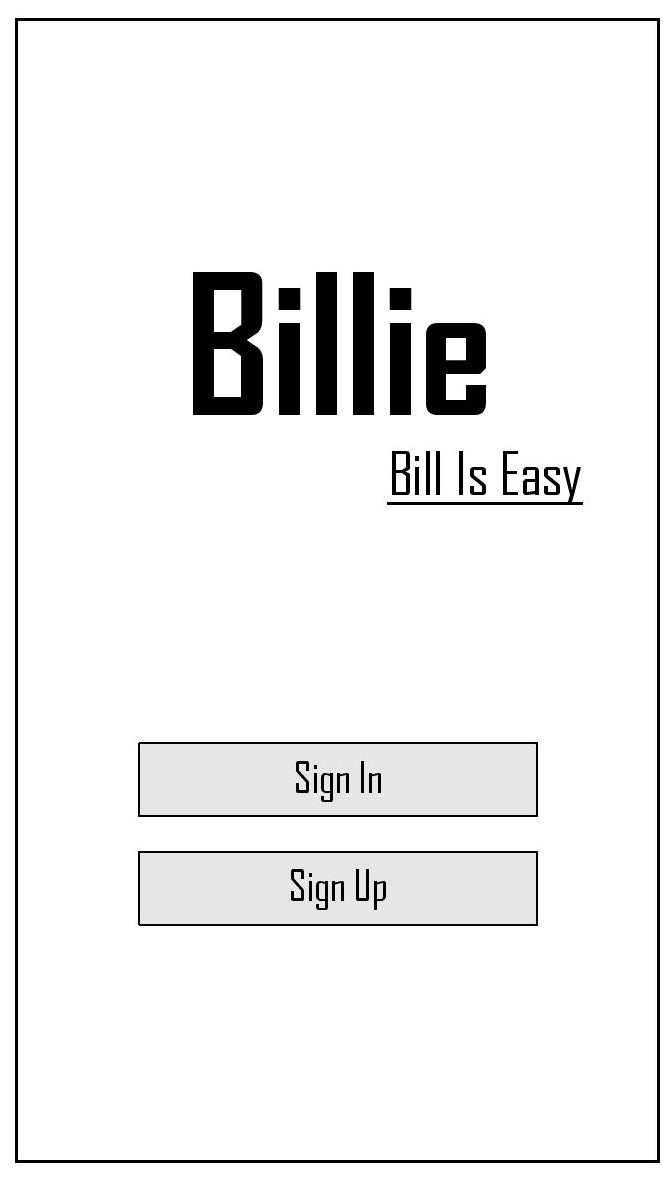
\includegraphics[width=0.5\columnwidth]{1.jpg}
  \caption{Q1}
  \label{fig:ADfigure1}
\end{figure}

\item You are on the welcome page now. 
    \begin{enumerate}
        \item You don't have an account yet. Now you want to sign up for an account. How would you do that?
        
        \begin{figure}[h!]
            \centering
             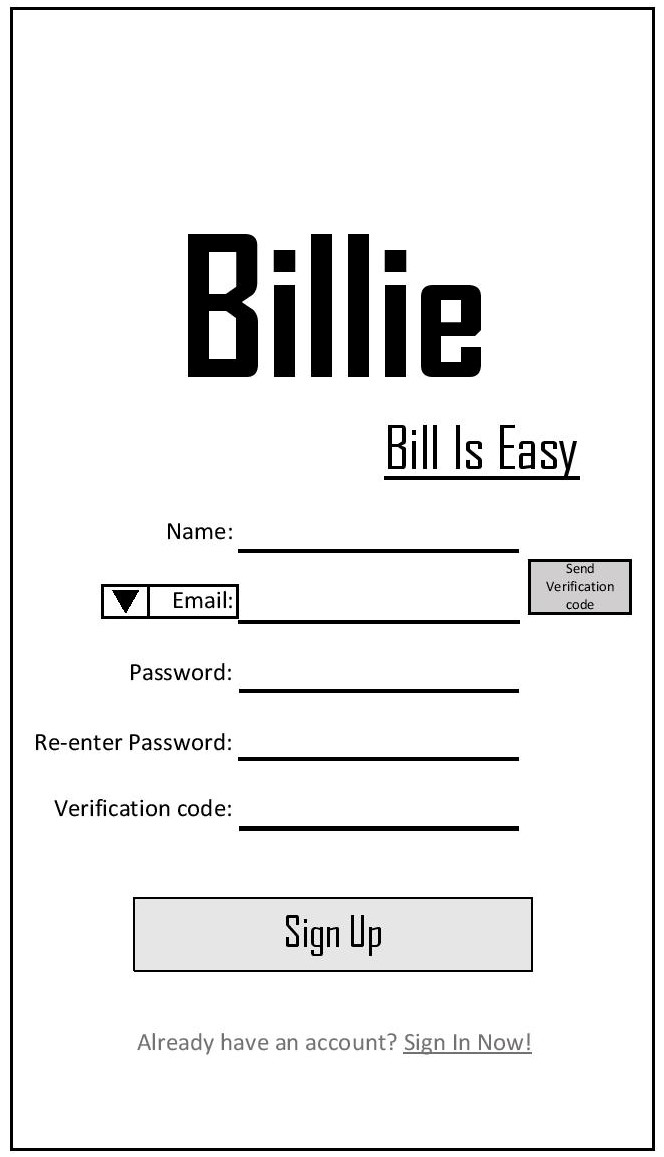
\includegraphics[width=0.5\columnwidth]{2-1.jpg}
             \caption{Q2}
             \label{fig:ADfigure2}
        \end{figure}

        \item You already have an account. Now sign in to your account. How would you do that?
        
        \begin{figure}[h!]
            \centering
             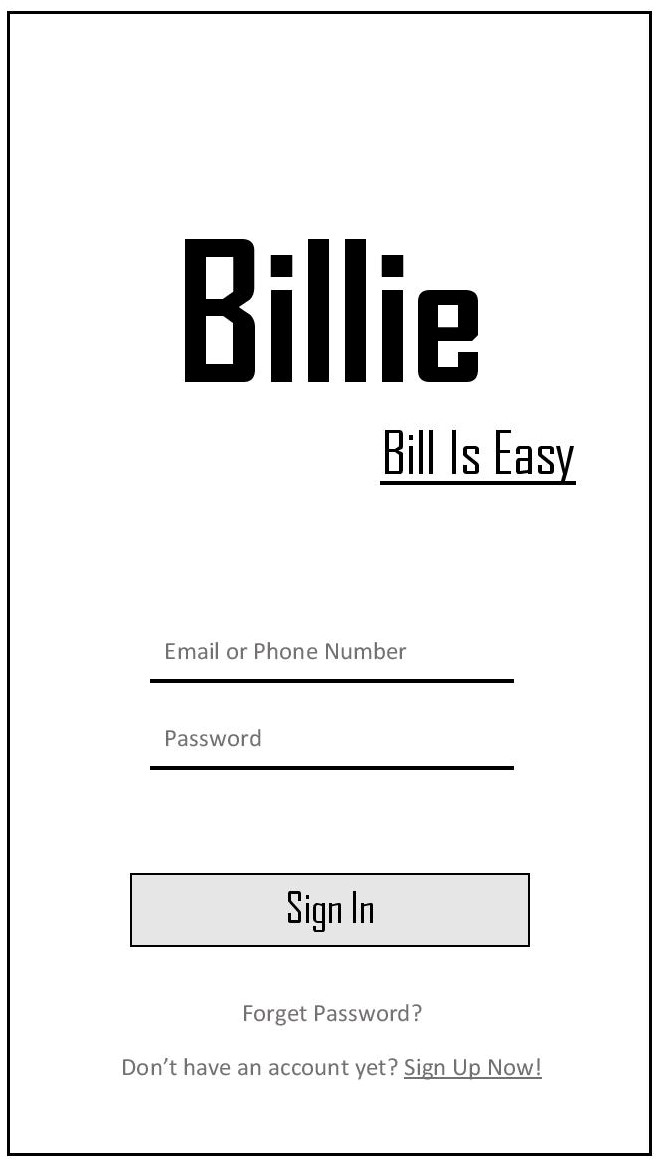
\includegraphics[width=0.5\columnwidth]{2-2.jpg}
             \caption{Q2}
             \label{fig:ADfigure3}
        \end{figure}
        
    \end{enumerate}
    \newpage
    
\item Now you are on the main/home page. You want to ensure that your account is as protected as possible. How would you do that?

\begin{figure}[h!]
\centering
  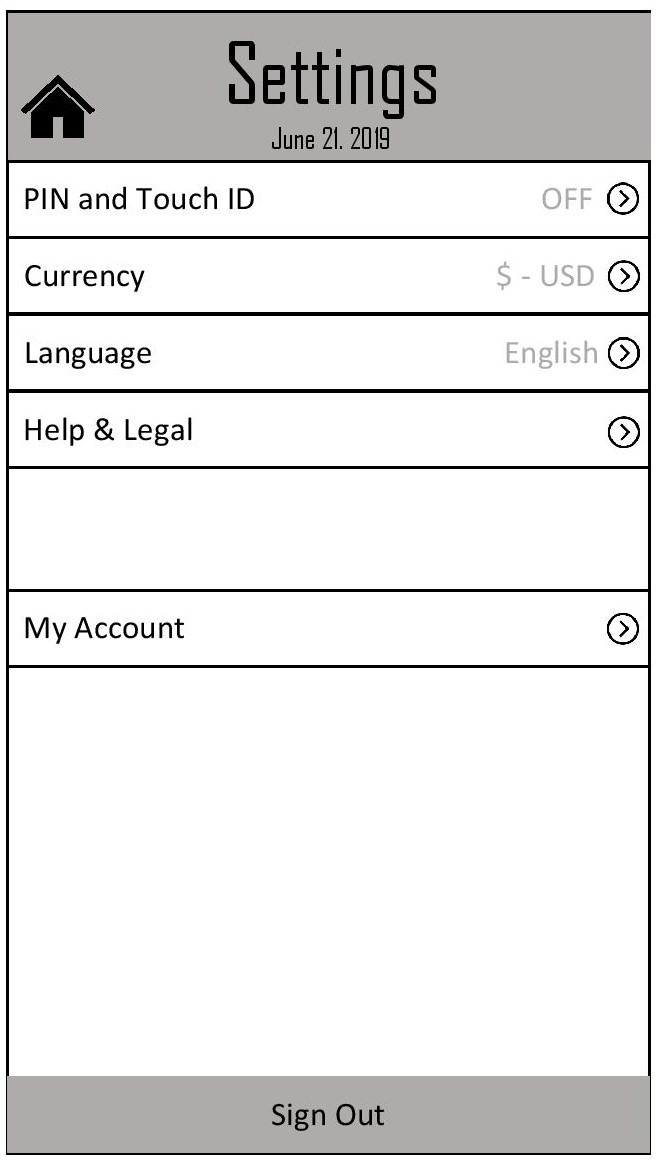
\includegraphics[width=0.5\columnwidth]{3-1.jpg}
  \caption{Q3}
  \label{fig:ADfigure4}
\end{figure}
\begin{figure}[h!]
\centering
  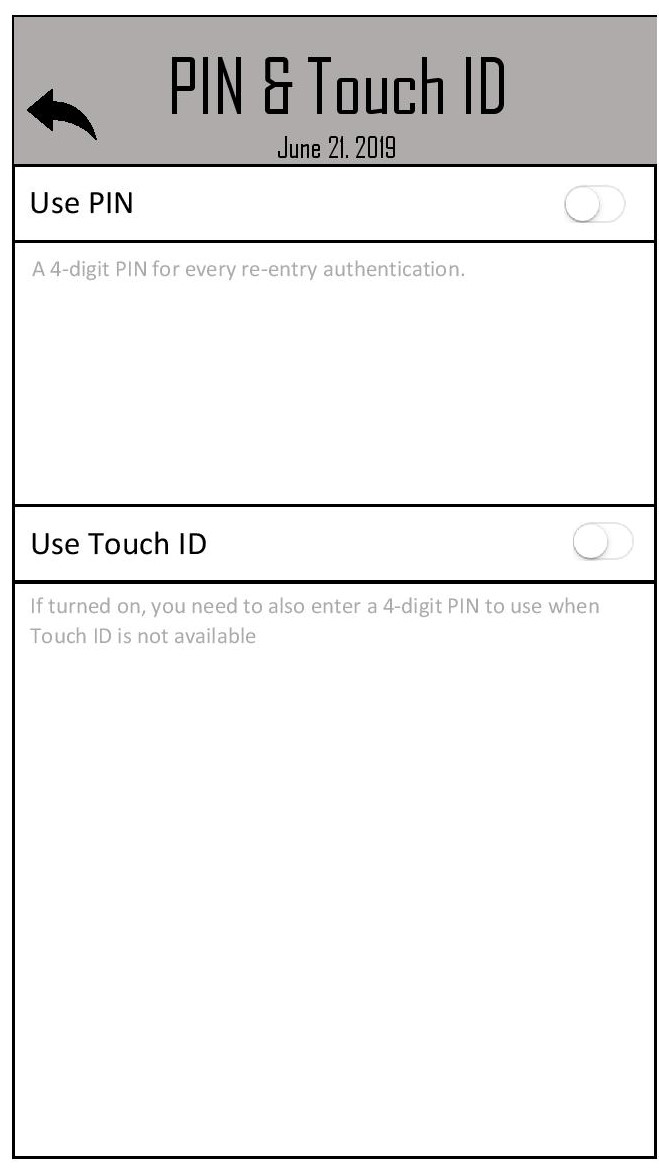
\includegraphics[width=0.5\columnwidth]{3-2.jpg}
  \caption{Q3}
  \label{fig:ADfigure5}
\end{figure}
\begin{figure}[h!]
\centering
  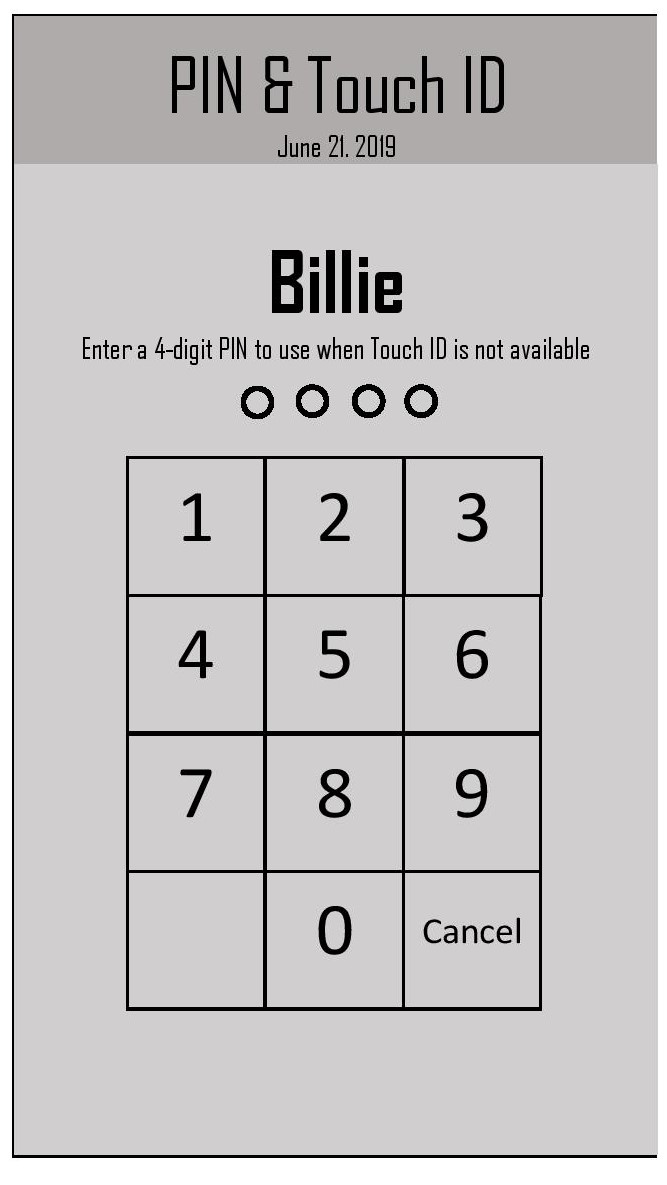
\includegraphics[width=0.5\columnwidth]{3-3.jpg}
  \caption{Q3}
  \label{fig:ADfigure6}
\end{figure}
\begin{figure}[h!]
\centering
  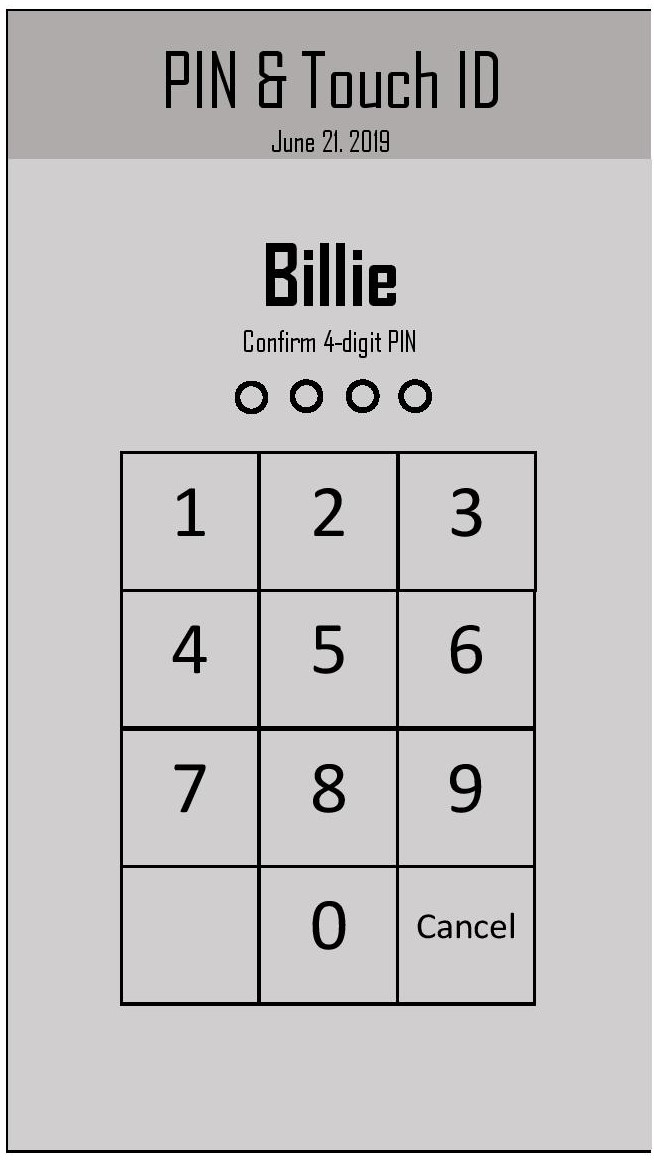
\includegraphics[width=0.5\columnwidth]{3-4.jpg}
  \caption{Q3}
  \label{fig:ADfigure7}
\end{figure}


\newpage
\newpage
\item You want to change the default currency to CAD. How would you do that?

\begin{figure}[h!]
\centering
  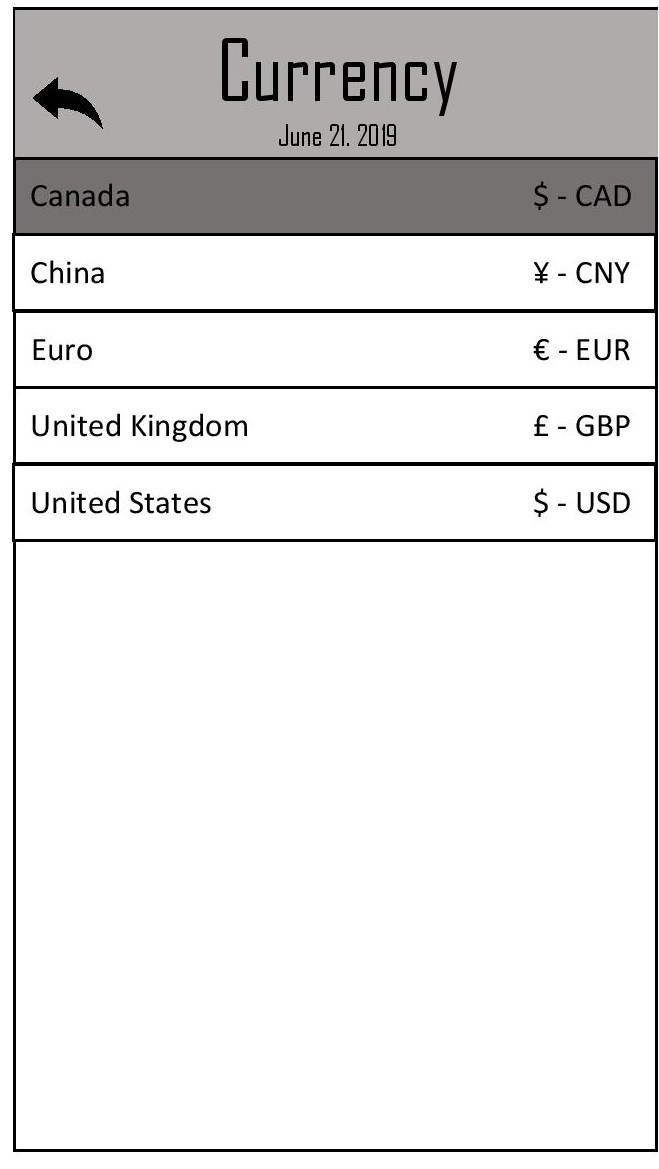
\includegraphics[width=0.5\columnwidth]{4.jpg}
  \caption{Q4}
  \label{fig:ADfigure8}
\end{figure}

\newpage
\item You want to get back to the main/home page. How would you do that?

\begin{figure}[h!]
\centering
  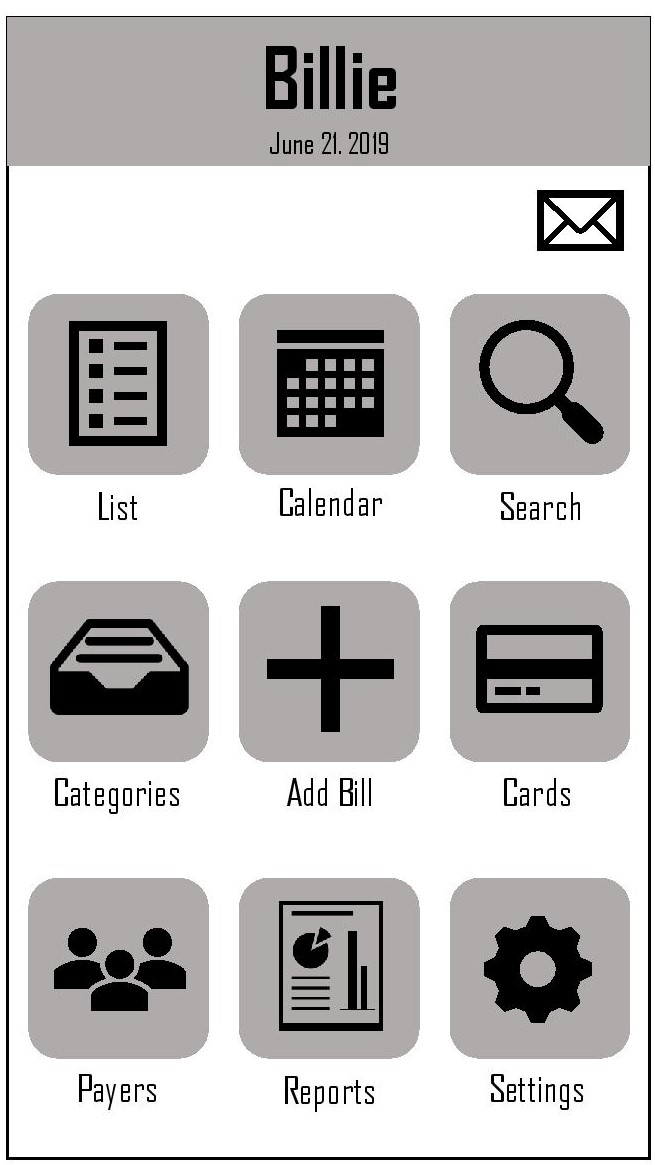
\includegraphics[width=0.5\columnwidth]{5.jpg}
  \caption{Q5}
  \label{fig:ADfigure9}
\end{figure}

\newpage
\item You switched to another application and now bring Billie back from the background.
    \begin{enumerate}
    \item Suppose biometric authentication is on and working. You want to enter Billie. How would you do that?
    \item Suppose biometric authentication is on but failed to work. You want to enter Billie. How would you do that?
    \end{enumerate}
    
    \begin{figure}[h!]
\centering
  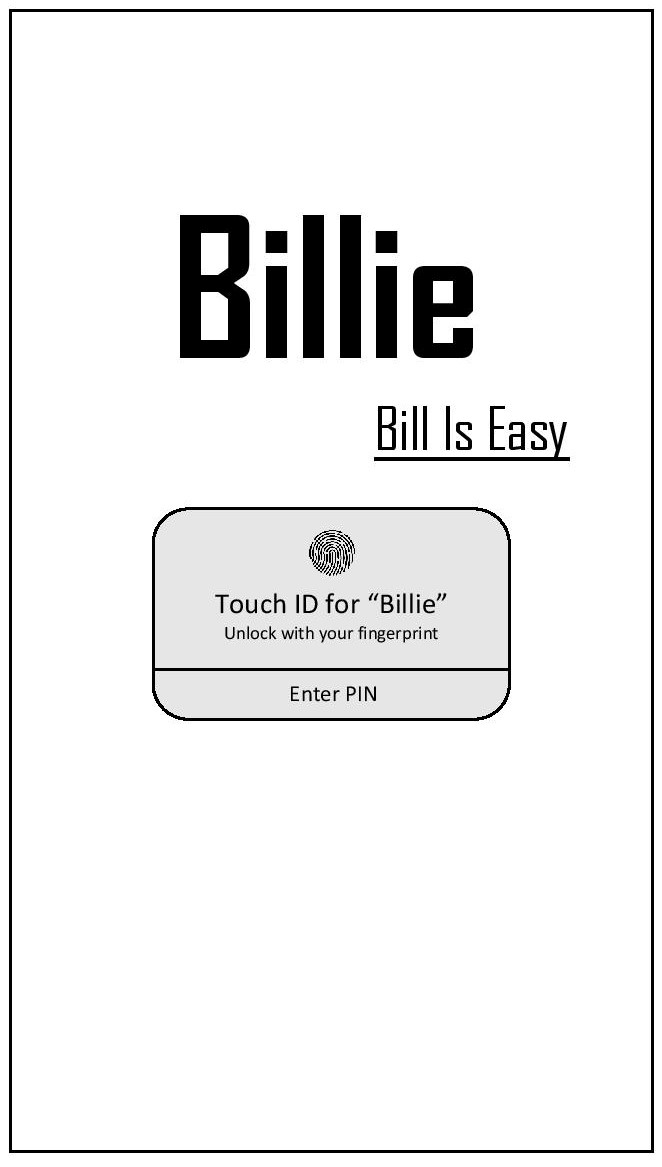
\includegraphics[width=0.5\columnwidth]{6.jpg}
  \caption{Q6}
  \label{fig:ADfigure10}
\end{figure}

\newpage
\item You just ate at a restaurant and got a receipt of a total value of \$15.33 paid with your previously saved CIBC debit card. You want to save a record of this bill by adding this bill to Billie. How would you do that?
\begin{figure}[h!]
\centering
  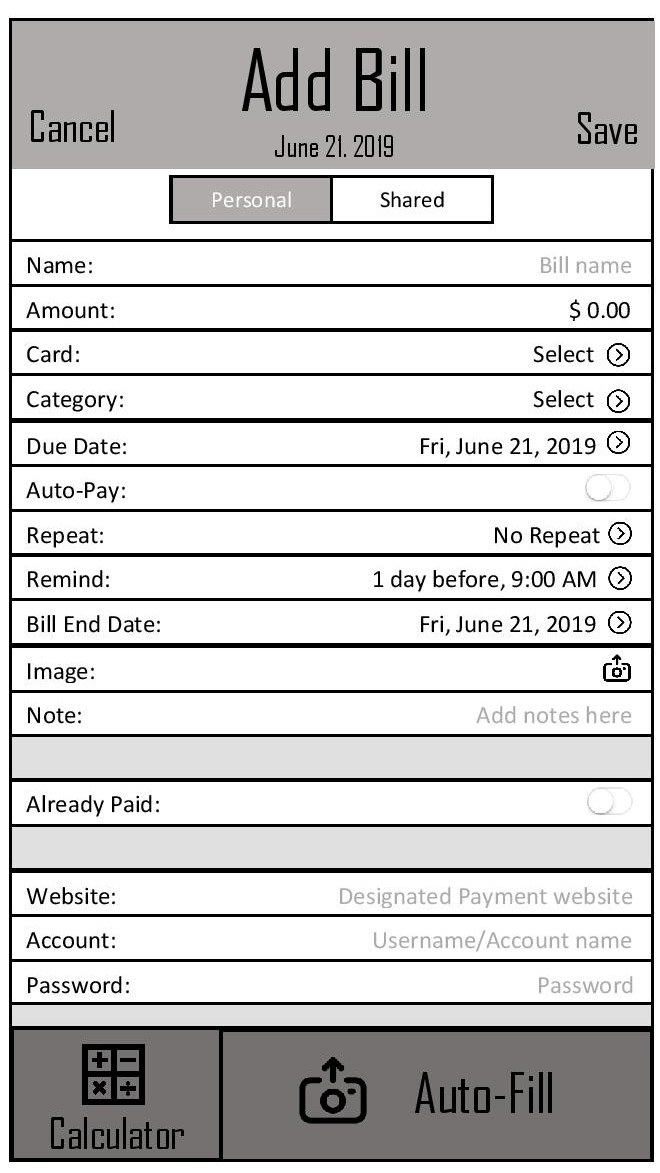
\includegraphics[width=0.5\columnwidth]{7-1.jpg}
  \caption{Q7}
  \label{fig:ADfigure11}
\end{figure}
\begin{figure}[h!]
\centering
  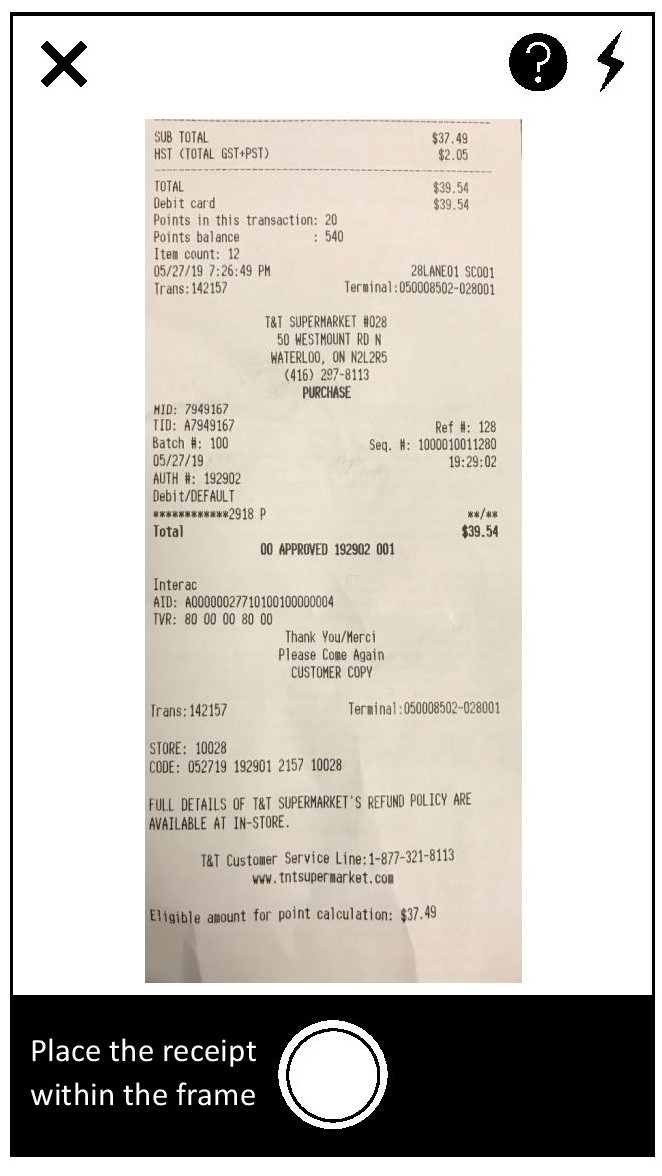
\includegraphics[width=0.5\columnwidth]{7-2.jpg}
  \caption{Q7}
  \label{fig:ADfigure12}
\end{figure}
\begin{figure}[h!]
\centering
  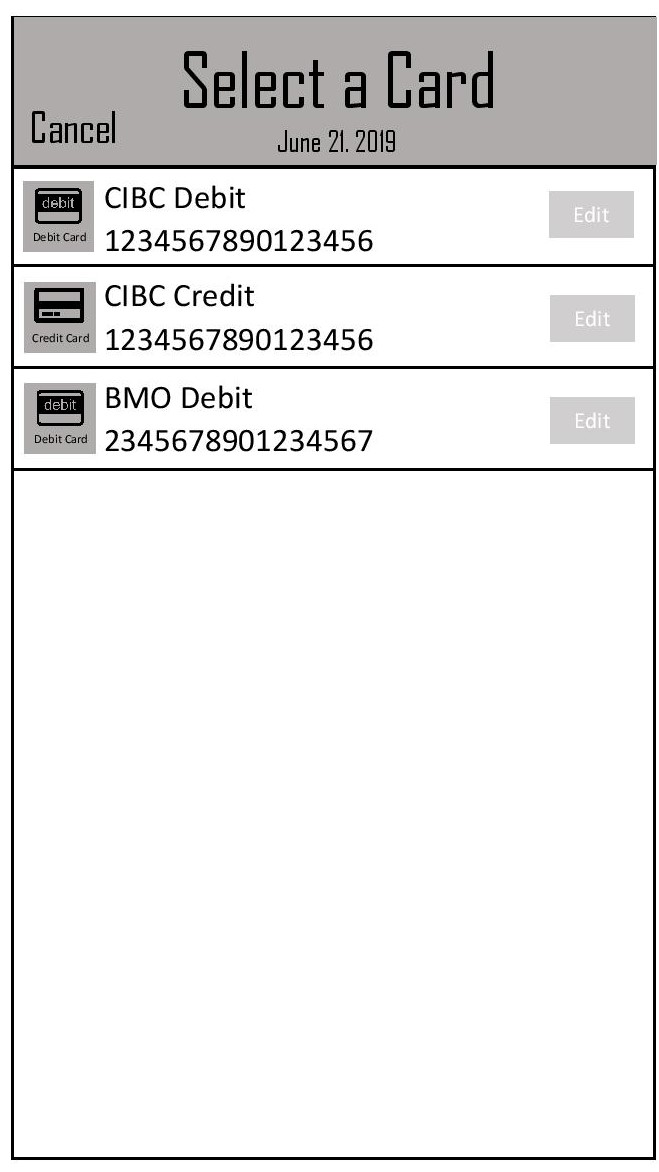
\includegraphics[width=0.5\columnwidth]{7-3.jpg}
  \caption{Q7}
  \label{fig:ADfigure13}
\end{figure}
\begin{figure}[h!]
\centering
  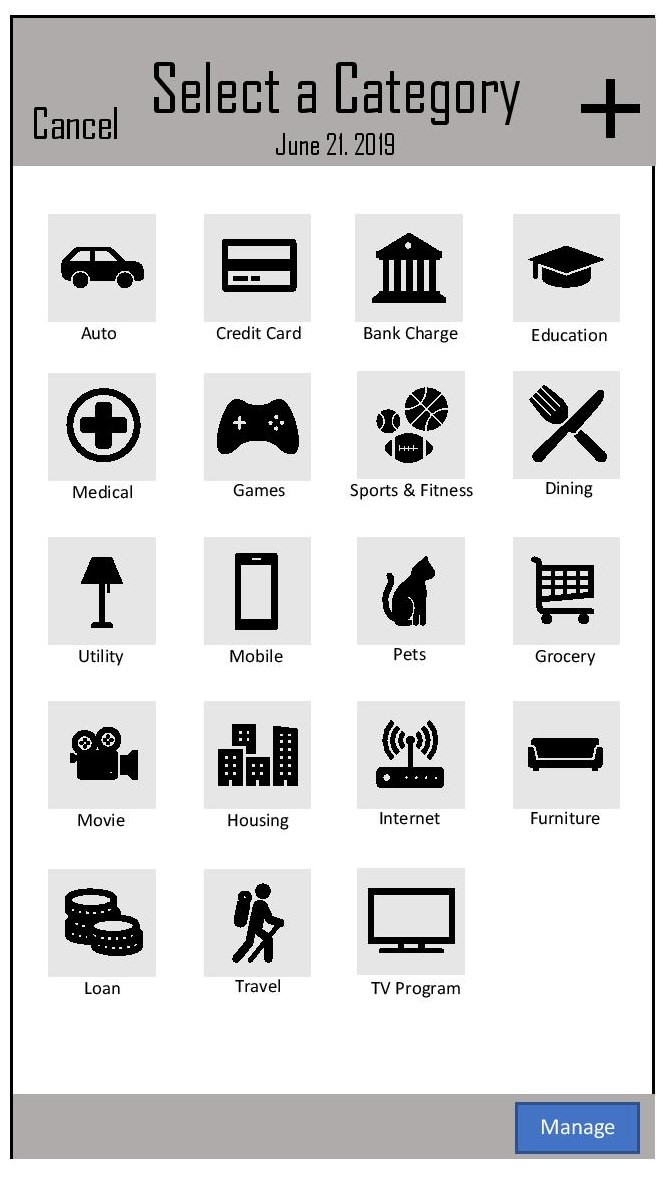
\includegraphics[width=0.5\columnwidth]{7-4.jpg}
  \caption{Q7}
  \label{fig:ADfigure14}
\end{figure}

\newpage
\item You had 3 friends came over last night and there is a total expense of \$87.58 paid with your new BMO credit card that you want to share evenly within your group of 4. How would you do that?

\begin{figure}[h!]
\centering
  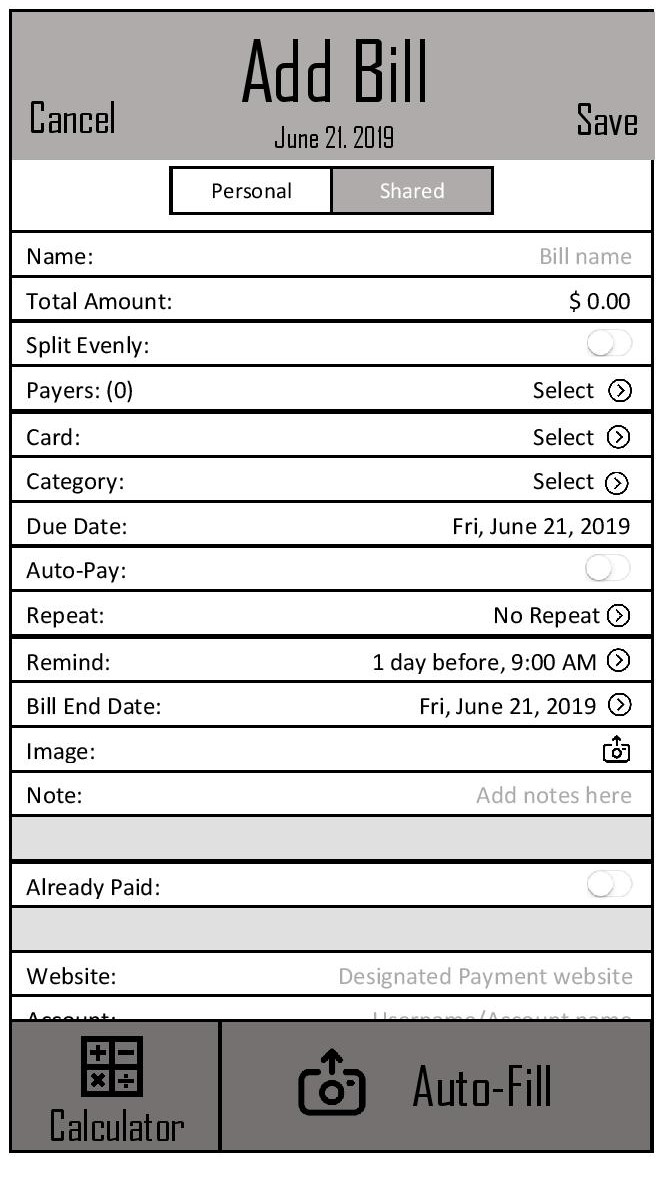
\includegraphics[width=0.5\columnwidth]{8-1.jpg}
  \caption{Q8}
  \label{fig:ADfigure15}
\end{figure}
\begin{figure}[h!]
\centering
  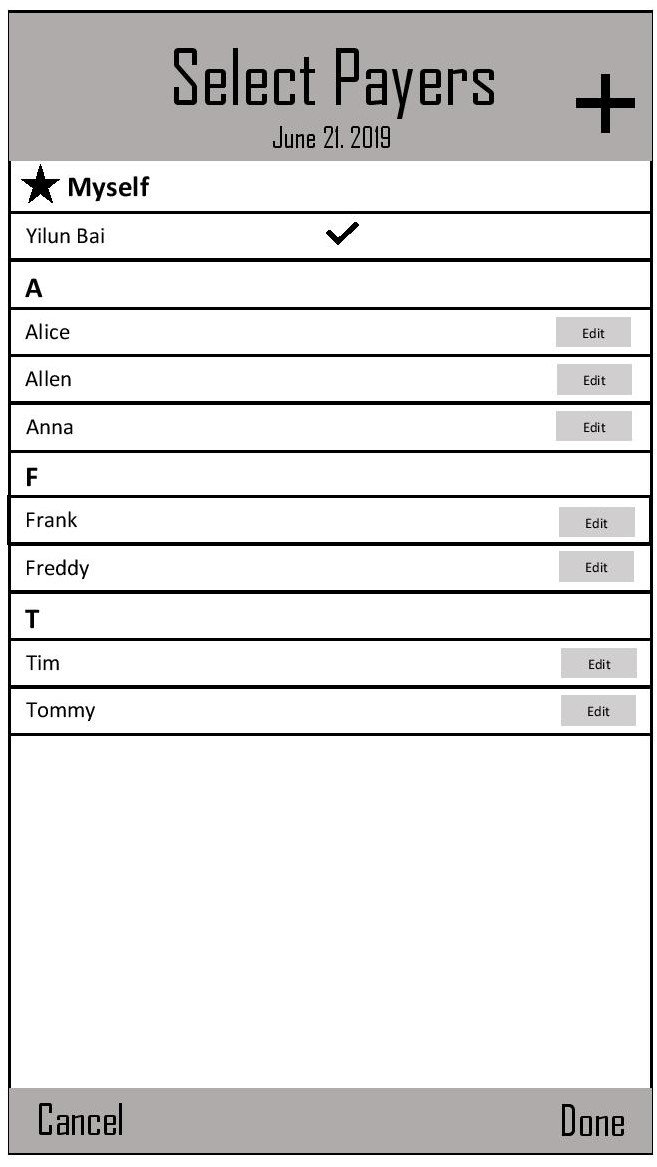
\includegraphics[width=0.5\columnwidth]{8-2.jpg}
  \caption{Q8}
  \label{fig:ADfigure16}
\end{figure}
\begin{figure}[h!]
\centering
  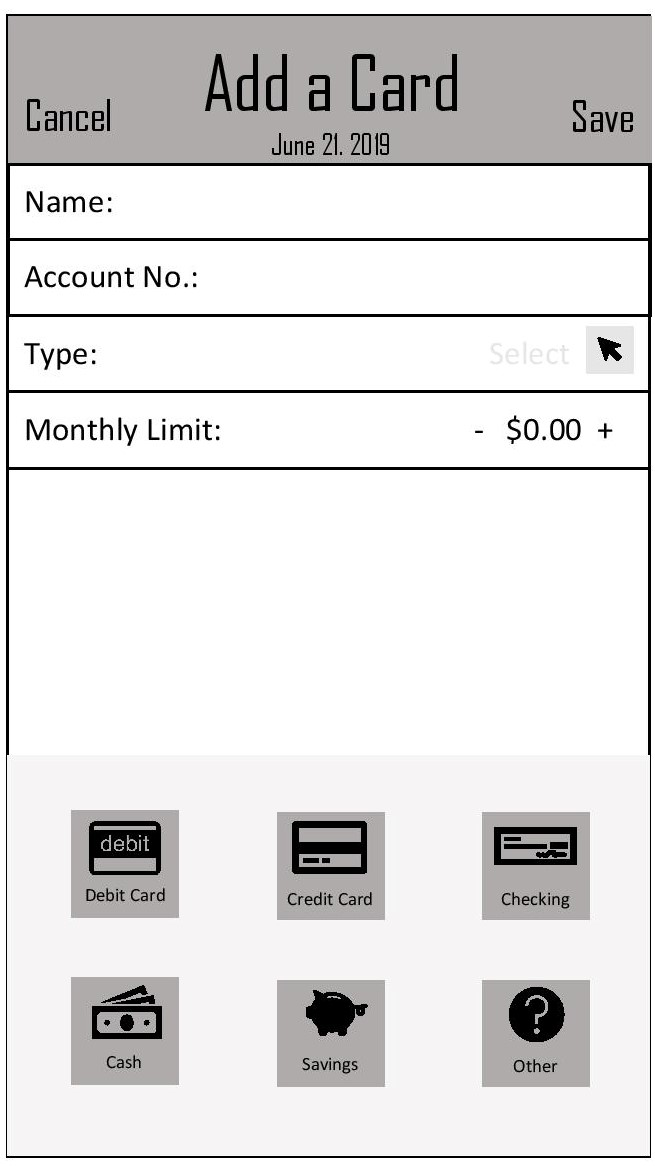
\includegraphics[width=0.5\columnwidth]{8-3.jpg}
  \caption{Q8}
  \label{fig:ADfigure17}
\end{figure}
\begin{figure}[h!]
\centering
  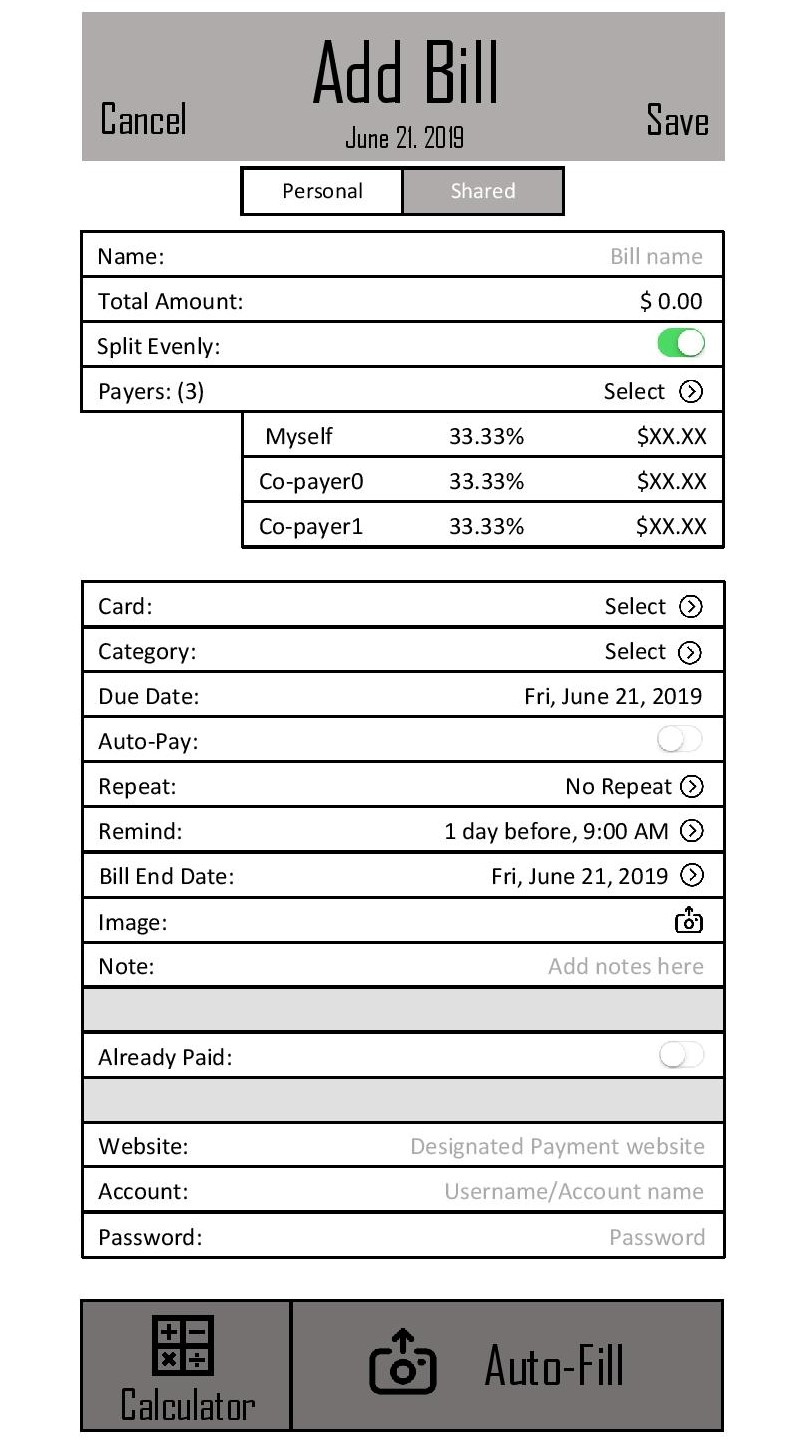
\includegraphics[width=0.5\columnwidth]{8-4.jpg}
  \caption{Q8}
  \label{fig:ADfigure18}
\end{figure}

\newpage
\item You want to view your expenses within the last week. How would you do that?

\begin{figure}[h!]
\centering
  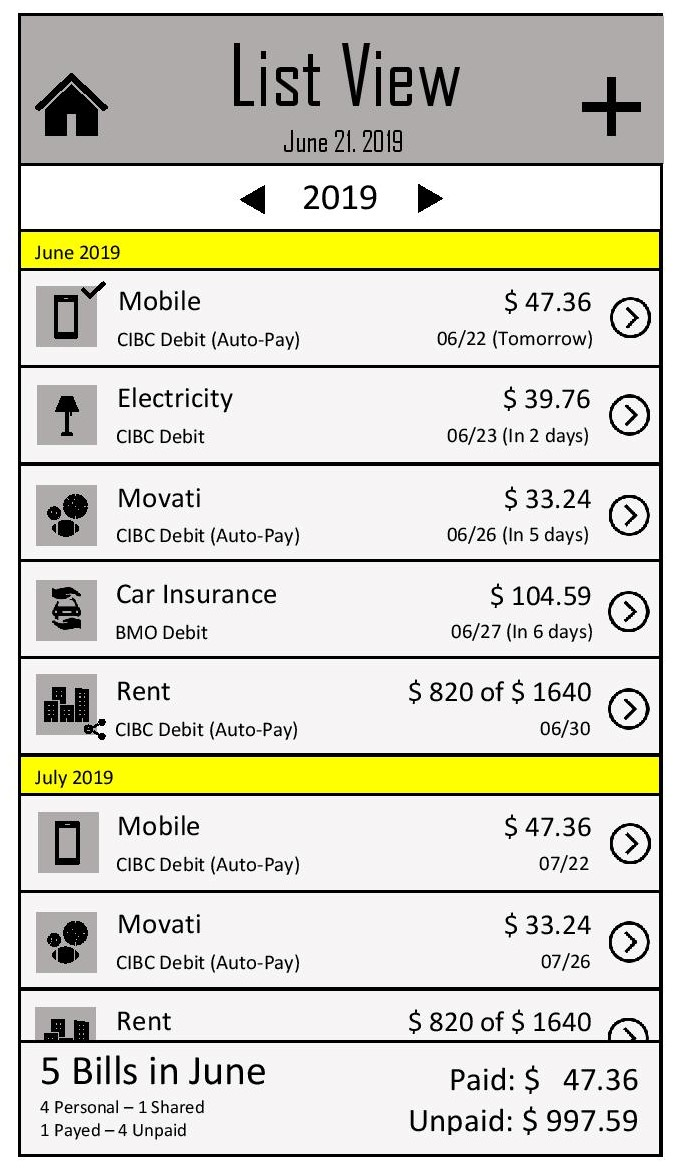
\includegraphics[width=0.5\columnwidth]{9.jpg}
  \caption{Q9}
  \label{fig:ADfigure19}
\end{figure}


\newpage
\item You want to view the upcoming bill dates. How would you do that?

\begin{figure}[h!]
\centering
  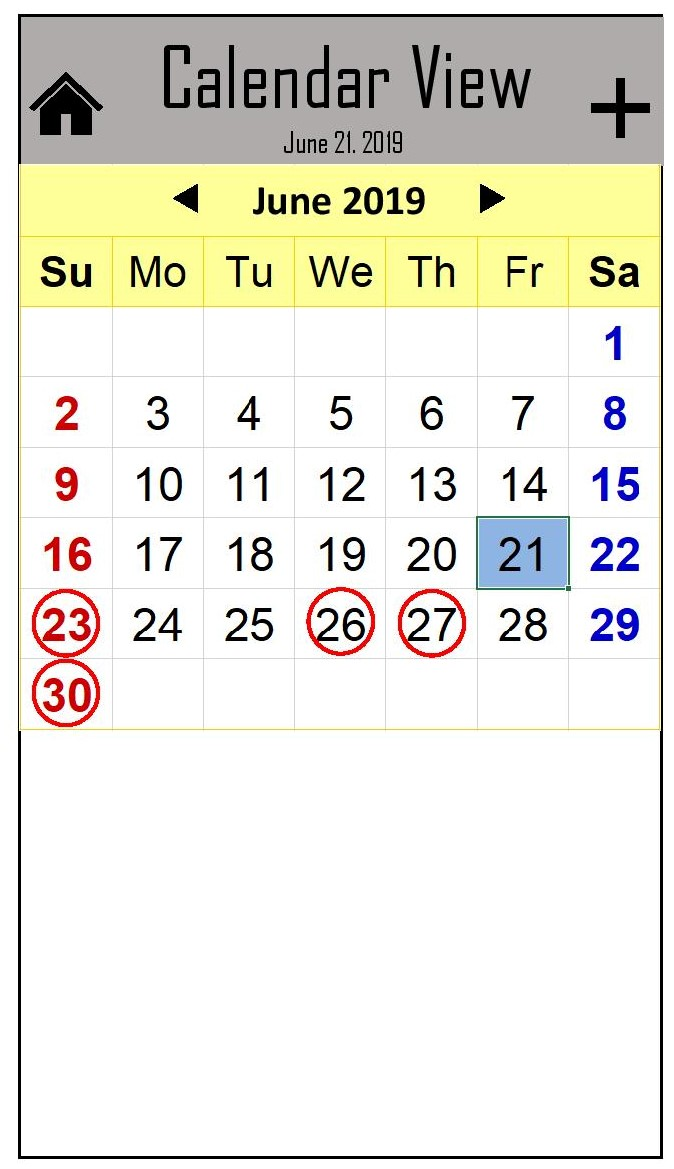
\includegraphics[width=0.5\columnwidth]{10.jpg}
  \caption{Q10}
  \label{fig:ADfigure20}
\end{figure}

\newpage
\item You locked your screen. Now you received a notification saying that you have an electricity bill of amount \$35.13 is about to due in 3 days. But you decide to pay it now within Billie. How would you do that?

\begin{figure}[h!]
\centering
  \includegraphics[width=0.4\columnwidth]{11-1.jpg}
  \caption{Q11}
  \label{fig:ADfigure21}
\end{figure}
\begin{figure}[h!]
\centering
  \includegraphics[width=0.4\columnwidth]{11-2.jpg}
  \caption{Q11}
  \label{fig:ADfigure22}
\end{figure}
\begin{figure}[h!]
\centering
  \includegraphics[width=0.4\columnwidth]{11-3.jpg}
  \caption{Q11}
  \label{fig:ADfigure23}
\end{figure}
\begin{figure}[h!]
\centering
  \includegraphics[width=0.4\columnwidth]{11-4.jpg}
  \caption{Q11}
  \label{fig:ADfigure24}
\end{figure}

\newpage
\item You want to view your bill report from May 1 - May 31, 2019. How would you do that?

\begin{figure}[h!]
\centering
  \includegraphics[width=0.4\columnwidth]{12-1.jpg}
  \caption{Q12}
  \label{fig:ADfigure25}
\end{figure}
\begin{figure}[h!]
\centering
  \includegraphics[width=0.4\columnwidth]{12-2.jpg}
  \caption{Q12}
  \label{fig:ADfigure26}
\end{figure}
\begin{figure}[h!]
\centering
  \includegraphics[width=0.4\columnwidth]{12-3.jpg}
  \caption{Q12}
  \label{fig:ADfigure27}
\end{figure}

\newpage
\item You found you spend too much recently. And you want to set a monthly limit on your card. How would you do that?
\begin{figure}[h!]
\centering
  \includegraphics[width=0.4\columnwidth]{13-1.jpg}
  \caption{Q13}
  \label{fig:ADfigure28}
\end{figure}
\begin{figure}[h!]
\centering
  \includegraphics[width=0.4\columnwidth]{13-2.jpg}
  \caption{Q13}
  \label{fig:ADfigure29}
\end{figure}

\newpage
\item Now you want to sign out of the account. How do you do that?
\begin{figure}[h!]
\centering
  \includegraphics[width=0.4\columnwidth]{14.jpg}
  \caption{Q14}
  \label{fig:ADfigure30}
\end{figure}

\end{enumerate}



 \newpage
 \newpage
 \subsection{3. Wireframes with Descriptive User Flow}
 To view individual pages of the wireframe, go to File "Team\_Billie\_Wireframes.pdf". To view large images of the wireframes with descriptive user flow, go to File "Team\_Billie\_User\_Flow.pdf".
 
 \begin{figure}[h!]
\centering
  \includegraphics[width=1\columnwidth]{User-flow-page-001.jpg}
  \caption{Billie Welcome, Sign In, Sign Up page}
  \label{fig:figure40}
\end{figure}
 \begin{figure}[h!]
\centering
  \includegraphics[width=1\columnwidth]{User-flow-page-002.jpg}
  \caption{Billie Home page, View bills feature with List and Calendar Views}
  \label{fig:figure41}
\end{figure} 
 \begin{figure}[h!]
\centering
  \includegraphics[width=1\columnwidth]{User-flow-page-003.jpg}
  \caption{Billie Add a Bill page (Personal), Auto-Fill feature}
  \label{fig:figure42}
\end{figure} 
 \begin{figure}[htbp!]
\centering
  \includegraphics[width=1\columnwidth]{User-flow-page-004.jpg}
  \caption{Billie Add a Bill page (Shared), Payers Selection page}
  \label{fig:figure43}
\end{figure} 
 \begin{figure}[htbp!]
\centering
  \includegraphics[width=1\columnwidth]{User-flow-page-005.jpg}
  \caption{Billie Group tab, Primary payer view, Co-payer view}
  \label{fig:figure44}
\end{figure} 
 \begin{figure}[h!]
\centering
  \includegraphics[width=1\columnwidth]{User-flow-page-006.jpg}
  \caption{Billie lock screen notification, Bill Alerts page }
  \label{fig:figure45}
\end{figure} 
 \begin{figure}[h!]
\centering
  \includegraphics[width=1\columnwidth]{User-flow-page-007.jpg}
  \caption{Billie "My" tab, "My Account" page}
  \label{fig:figure46}
\end{figure} 
 \begin{figure}[h!]
\centering
  \includegraphics[width=1\columnwidth]{User-flow-page-008.jpg}
  \caption{Billie "Categories", "Add a Category", "Edit a Category" page}
  \label{fig:figure47}
\end{figure} 
 \begin{figure}[h!]
\centering
  \includegraphics[width=1\columnwidth]{User-flow-page-009.jpg}
  \caption{Billie "Cards", "Add a Card", "Edit a Card" page}
  \label{fig:figure48}
\end{figure} 
 \begin{figure}[h!]
\centering
  \includegraphics[width=1\columnwidth]{User-flow-page-010.jpg}
  \caption{Billie "Payers", "Add a Payer", "Edit a Payer" page}
  \label{fig:figure49}
\end{figure} 
 \begin{figure}[h!]
\centering
  \includegraphics[width=1\columnwidth]{User-flow-page-011.jpg}
  \caption{Billie "Report" pages with different reports during different time span}
  \label{fig:figure50}
\end{figure} 
 \begin{figure}[h!]
\centering
  \includegraphics[width=1\columnwidth]{User-flow-page-012.jpg}
  \caption{Billie "Settings" page with PIN and Touch ID set up process, "Currency" page}
  \label{fig:figure51}
\end{figure} 


\clearpage


\begin{figure*}[h!]
  \subsection{4. Affinity diagram}
  \centering
  \includegraphics[width=\textwidth]{Affinity_Diagram.png}
  \caption{Affinity Diagram}
  \label{fig:figure7}
\end{figure*}



\clearpage
\newpage

\begin{figure*}[t!]
\subsection{5. Work models}
\centering
  \includegraphics[width=\textwidth,height=13cm]{Cultural_Model.png}
  \caption{Cultural Model}
  \label{fig:WMfigure10}
\end{figure*}


\begin{figure*}[h]
\centering
  \includegraphics[width=\textwidth,height=13cm]{Flow_Model.png}
  \caption{Flow Model}
  \label{fig:WMfigure11}
\end{figure*}


\end{document}